\documentclass[runningheads]{llncs}

\usepackage{graphicx}
\usepackage{amsmath,amssymb,amsfonts}
\usepackage{algorithmic}
\usepackage{textcomp}
\usepackage{xcolor}
\usepackage{url}
\usepackage{booktabs}
\usepackage{array}
\usepackage{multirow}
\usepackage{float}
\usepackage{subcaption}
\usepackage{stfloats}
\usepackage{placeins}
\usepackage{enumitem}
\setlist{nosep}
\usepackage{caption}
\captionsetup[figure]{font=small,skip=2pt}
\captionsetup[subcaption]{font=small,skip=1pt}



% Reduce spacing around equations
\setlength{\abovedisplayskip}{6pt}
\setlength{\belowdisplayskip}{6pt}
\setlength{\abovedisplayshortskip}{3pt}
\setlength{\belowdisplayshortskip}{3pt}

% Reduce spacing around floats (figures/tables)
\setlength{\textfloatsep}{8pt plus 2pt minus 2pt}
\setlength{\floatsep}{8pt plus 2pt minus 2pt}
\setlength{\intextsep}{6pt plus 2pt minus 2pt}
\setlength{\dbltextfloatsep}{8pt plus 2pt minus 2pt}
\setlength{\dblfloatsep}{8pt plus 2pt minus 2pt}

\begin{document}

\titlerunning{Deepfake Detection on Facial Features}
\authorrunning{E. S. Pokharia et al.}

\title{Deepfake Detection on Facial Features Using Deep Learning: A Comparative Study of CNN and Transformer Architectures}

\author{Eeshan Singh Pokharia\inst{1}\orcidID{} \and
Soumya Mukherjee\inst{1}\orcidID{} \and
Jayendra Singh\inst{1}\orcidID{} \and
Manoj Patra\inst{2}\orcidID{} \and
Ankit Jain\inst{1}\orcidID{} \and
Shiv Prasad\inst{1}\orcidID{}}

\institute{Department of Computer and Communication Engineering,
The LNM Institute of Information and Technology, Jaipur, India\\
\email{\{23ucc540,soumya.mukherjee,ankit.jain,psad.shiv\}@lnmiit.ac.in}
\and
Department of Computer Science and Engineering,
National Institute of Technology, Warangal, India}

\maketitle

\begin{abstract}
The rapid growth of synthetic media technologies, especially deepfakes, poses a serious threat to the credibility of online content. This study provides a practical comparison of four different deep learning models aimed at detecting manipulated faces: EfficientNet-B0, XceptionNet, ResNet50, and the Vision Transformer (ViT). Authors used the Celeb-DF dataset to train these models, achieving testing accuracies of 98.70\%, 98.76\%, 98.22\%, and 90.54\%, respectively. To evaluate how well these models deal with new data, authors conducted cross-dataset validation using FaceForensics++. The results showed a general drop in performance; however, the Vision Transformer showed better resilience. While the CNN-based models faced accuracy drops over 40\%, the ViT's accuracy decreased by only 24.48\%. Authors also used Gradient-weighted Class Activation Mapping (Grad-CAM) to visualize how the models make decisions, confirming that all models focus correctly on facial areas. These results suggest that while CNNs perform well with familiar data, transformer-based models may adjust better to changes in data distribution. This shows the need to test across different datasets to develop reliable forensic tools.
\end{abstract}

\keywords{deepfake detection \and deep learning \and computer vision \and convolutional neural networks \and vision transformers \and model interpretability \and cross-dataset evaluation}

\section{Introduction}
The technology for creating synthetic media has grown from early academic experiments to publicly available tools that can produce hyperrealistic fake videos and images. These manipulations, commonly known as deepfakes, use machine learning to alter visual content with convincing accuracy. The concerns stretch beyond entertainment into privacy violations, political disinformation, and identity theft \cite{deepfake_survey}. As generative models like GANs continue to improve, building reliable detection systems has become essential.

Early detection approaches tried to find specific artifacts. Li et al. proposed exposing fake videos by detecting unnatural eye blinking patterns \cite{frequency_domain}, while Afchar et al. introduced MesoNet, a compact CNN that could detect deepfakes with relatively few parameters \cite{mesonet}. The FaceForensics++ benchmark by Rössler et al. helped standardize how detection methods are evaluated by offering a large collection of videos manipulated using multiple techniques \cite{faceforensics}. As the field progressed, Convolutional Neural Networks became the primary approach. XceptionNet used depthwise separable convolutions for efficient feature extraction \cite{xception_deepfake}. EfficientNet improved performance through compound scaling without significantly raising computational costs \cite{efficientnet}. ResNet architectures remain popular because their skip connections help gradients flow through deep networks \cite{resnet_deepfake}. More recently, Vision Transformers have been adapted for vision tasks by treating images as sequences of patches \cite{vit}, though their use in deepfake detection has been less explored compared to CNNs. A key challenge remains the generalization gap --- models tend to perform well on their training data but fail when faced with deepfakes from different sources or algorithms \cite{cross_dataset}. This highlights the tendency to overfit on specific dataset artifacts rather than learning what truly separates real from fake content.

The goal of this paper is to systematically compare four architectures --- EfficientNet-B0, XceptionNet, ResNet50, and the Vision Transformer --- for deepfake detection. Authors trained models on the Celeb-DF dataset and tested them on FaceForensics++ to evaluate their generalization. Grad-CAM was used to visualize how each model makes its decisions.

\section{Contributions and Novelty}
To our knowledge, this is the first systematic comparison of EfficientNet-B0, XceptionNet, ResNet50, and Vision Transformer architectures for deepfake detection under identical training conditions with cross-dataset evaluation. This work advances the field through the following contributions:

\begin{enumerate}
    \item \textbf{Comparative Benchmarking:} Authors provide a controlled comparison of four distinct architectures under identical training constraints to ensure a fair assessment.

    \item \textbf{Robustness Analysis:} Authors rigorously test generalization by training on Celeb-DF and evaluating on the unseen FaceForensics++ dataset, exposing the real-world limitations of these models.

    \item \textbf{Key Finding on ViT Generalization:} Authors demonstrate that Vision Transformers exhibit significantly better cross-dataset resilience, with only a 24.48\% accuracy drop compared to over 42\% for CNNs.

    \item \textbf{Model Interpretability:} Using Grad-CAM, Authors visualize the attention maps of all four models, confirming that they focus on facial features rather than background noise.

    \item \textbf{Reproducibility:} Authors present a full, repeatable pipeline from preprocessing to evaluation to aid future research.
\end{enumerate}

\section{Proposed Work}

\subsection{Dataset}
Authors utilized two prominent datasets for this study:

\textbf{Celeb-DF (v2):} This dataset contains 590 real videos and 5,639 fake videos, known for its high visual quality and realistic manipulations \cite{cross_dataset}. After preprocessing, authors obtained 1,736 real and 16,736 fake face images, totaling 18,472 images. An 80-10-10 split was used for training, validation, and testing.

\textbf{FaceForensics++:} This benchmark includes 1,000 original sequences manipulated by six methods such as Face2Face and NeuralTextures \cite{faceforensics}. Authors extracted 2,992 real and 17,789 fake images, making a total of 20,781. This dataset was used only for testing to evaluate cross-dataset generalization.

\subsection{Preprocessing Pipeline}
To ensure the models focused solely on facial features, authors standardized the data input:

\begin{enumerate}
    \item \textbf{Frame Sampling:} Authors extracted frames at regular intervals. Authors took every 30th frame for Celeb-DF and every 60th frame for FaceForensics++ to control the amount of data.

    \item \textbf{Face Localization:} Authors used OpenCV's Haar Cascade to automatically find faces in the frames.

    \item \textbf{Cropping:} Authors cropped the detected faces with a 20\% margin. This included the immediate boundary of the face, where blending artifacts often show up.

    \item \textbf{Resizing:} Images were resized to 224$\times$224 pixels.

    \item \textbf{Normalization:} Pixel intensities were scaled to the [0, 1] range.
\end{enumerate}

\subsection{Model Architectures}

\subsubsection{EfficientNet-B0}
This model uses a compound scaling method to improve depth, width, and resolution at the same time. With about 4.6 million parameters, it is the lightest model authors tested, which makes it suitable for situations with limited computing power.

\subsubsection{XceptionNet}
XceptionNet replaces standard convolutions with depthwise separable convolutions. This change makes the model more efficient while keeping strong feature extraction abilities. It has around 38.9 million parameters and is commonly used as a baseline in deepfake research.

\subsubsection{ResNet50}
ResNet50 uses skip connections, also known as residuals. These connections help gradients flow more easily during backpropagation. The structure has about 25 million parameters and addresses the degradation issue in deeper networks.

\subsubsection{Vision Transformer (ViT)}
Unlike CNNs, ViT treats an image as a sequence of patches. An image $\mathbf{x} \in \mathbb{R}^{H \times W \times C}$ is split into $N$ patches of size $P \times P$. These are flattened and projected:
\begin{equation}
\mathbf{z}_0 = [\mathbf{x}_{\text{class}}; \mathbf{x}_p^1\mathbf{E}; \mathbf{x}_p^2\mathbf{E}; \ldots; \mathbf{x}_p^N\mathbf{E}] + \mathbf{E}_{\text{pos}}
\label{eq:vit_patches}
\end{equation}
Here, $\mathbf{x}_{\text{class}}$ is the classification token, $\mathbf{E}$ is the patch embedding matrix, and $\mathbf{E}_{\text{pos}}$ is the positional embedding. The data flows through transformer encoders containing Multi-Head Self-Attention (MSA) and Multi-Layer Perceptron (MLP) blocks:
\begin{align}
\mathbf{z}'_l &= \text{MSA}(\text{LN}(\mathbf{z}_{l-1})) + \mathbf{z}_{l-1} \\
\mathbf{z}_l &= \text{MLP}(\text{LN}(\mathbf{z}'_l)) + \mathbf{z}'_l
\label{eq:vit_encoder}
\end{align}
where LN denotes layer normalization. The attention mechanism allows the model to relate distant parts of the image globally:
\begin{equation}
\text{MSA}(\mathbf{z}) = [\text{head}_1; \text{head}_2; \ldots; \text{head}_h]\mathbf{W}^O
\label{eq:vit_msa}
\end{equation}
where each head computes attention as in Equation~\eqref{eq:attention}, and $\mathbf{W}^O$ is the output projection matrix.
With roughly 86 million parameters, ViT is the heaviest model but offers a completely different approach to feature analysis.

\subsection{Training Configuration}
The training setup was standardized as follows:

\subsubsection{Loss Function}
Authors used Binary Cross-Entropy loss:
\begin{equation}
\mathcal{L}_{CE} = -\frac{1}{N}\sum_{i=1}^{N}\left[y_i \log(\hat{y}_i) + (1-y_i)\log(1-\hat{y}_i)\right]
\label{eq:cross_entropy}
\end{equation}
where $y_i \in \{0,1\}$ is the ground truth label and $\hat{y}_i \in [0,1]$ is the predicted probability for sample $i$.

\subsubsection{Optimization}
ResNet50 utilized the AdamW optimizer, while the others used standard Adam. The Adam update rule is:
\begin{align}
m_t &= \beta_1 m_{t-1} + (1-\beta_1) g_t \\
v_t &= \beta_2 v_{t-1} + (1-\beta_2) g_t^2 \\
\hat{m}_t &= \frac{m_t}{1-\beta_1^t}, \quad \hat{v}_t = \frac{v_t}{1-\beta_2^t} \\
\theta_{t+1} &= \theta_t - \frac{\eta}{\sqrt{\hat{v}_t} + \epsilon}\hat{m}_t
\label{eq:adam}
\end{align}
where $g_t$ is the gradient at time step $t$, $\beta_1$ and $\beta_2$ are momentum decay rates (typically 0.9 and 0.999), $\eta$ is the learning rate, and $\epsilon$ is a small constant (typically $10^{-8}$) to prevent division by zero. AdamW adds decoupled weight decay for better regularization:
\begin{equation}
\theta_{t+1} = \theta_t - \frac{\eta}{\sqrt{\hat{v}_t} + \epsilon}\hat{m}_t - \lambda \eta \theta_t
\label{eq:adamw}
\end{equation}
where $\lambda$ is the weight decay coefficient.

\subsubsection{Learning Rate Scheduling}
Authors used Cosine Annealing for EfficientNet, Xception, and ViT:
\begin{equation}
\eta_t = \eta_{\min} + (\eta_{\max} - \eta_{\min}) \cdot \frac{1 + \cos(\pi t / T)}{2}
\label{eq:cosine_annealing}
\end{equation}
where $\eta_t$ is the learning rate at epoch $t$, $\eta_{\min}$ and $\eta_{\max}$ are the minimum and maximum learning rates, and $T$ is the total number of epochs. ResNet50 used a ReduceLROnPlateau scheduler:
\begin{equation}
\eta_{t+1} = \begin{cases}
\gamma \eta_t & \text{if validation metric does not improve} \\
\eta_t & \text{otherwise}
\end{cases}
\label{eq:plateau}
\end{equation}
where $\gamma$ is the reduction factor (typically 0.1 or 0.5).

\subsubsection{Training Hyperparameters}
\begin{itemize}
    \item \textbf{Learning Rate:} 1$\times$10$^{-4}$ (EfficientNet, Xception, ViT); 5$\times$10$^{-5}$ (ResNet50).
    \item \textbf{Batch Size:} 32.
    \item \textbf{Regularization:} Early stopping (patience 10-20 epochs).
    \item \textbf{Precision:} Mixed precision was used to speed up training.
\end{itemize}

\subsection{Evaluation Metrics}
To measure performance, authors tracked several metrics. Let $TP, TN, FP, FN$ stand for True Positives, True Negatives, False Positives, and False Negatives.

\subsubsection{Classification Metrics}
\textbf{Accuracy} is the overall correctness:
\begin{equation}
\text{Accuracy} = \frac{1}{N}\sum_{i=1}^{N}\mathbb{I}(y_i = \hat{y}_i) = \frac{TP + TN}{TP + TN + FP + FN}
\label{eq:accuracy}
\end{equation}

\textbf{Precision} indicates the quality of positive predictions:
\begin{equation}
\text{Precision} = \frac{TP}{TP + FP}
\label{eq:precision}
\end{equation}

\textbf{Recall} indicates the quantity of positives found:
\begin{equation}
\text{Recall} = \frac{TP}{TP + FN}
\label{eq:recall}
\end{equation}

\textbf{F1-Score} balances precision and recall:
\begin{equation}
\text{F1-Score} = 2 \cdot \frac{\text{Precision} \cdot \text{Recall}}{\text{Precision} + \text{Recall}} = \frac{2TP}{2TP + FP + FN}
\label{eq:f1}
\end{equation}

\subsubsection{Probabilistic Metrics}
\textbf{AUC-ROC} evaluates the model across all thresholds. It relies on True Positive Rate (TPR) and False Positive Rate (FPR):
\begin{align}
\text{TPR}(\tau) &= \frac{|\{i: p_i \geq \tau \text{ and } y_i = 1\}|}{|\{i: y_i = 1\}|} \\
\text{FPR}(\tau) &= \frac{|\{i: p_i \geq \tau \text{ and } y_i = 0\}|}{|\{i: y_i = 0\}|
\end{align}
where $\tau$ is the classification threshold, $p_i$ is the predicted probability for sample $i$, and $y_i$ is the true label. The Area Under the Curve is:
\begin{equation}
\text{AUC-ROC} = \int_{0}^{1} \text{TPR}(\text{FPR}^{-1}(u)) \, du
\label{eq:auc_roc}
\end{equation}
which measures the model's ability to distinguish between classes across all possible threshold values.

\subsection{Model Interpretability}
Authors employed Grad-CAM to ensure the models weren't cheating by looking at backgrounds.

\subsubsection{Grad-CAM Formulation}
For CNNs, authors calculate the importance $\alpha_k^c$ of feature map $A^k$ for class $c$:
\begin{equation}
\alpha_k^c = \frac{1}{HW}\sum_{i=1}^{H}\sum_{j=1}^{W}\frac{\partial y^c}{\partial A_{ij}^k}
\label{eq:gradcam_alpha}
\end{equation}
where $H$ and $W$ are the spatial dimensions of the feature map, and $y^c$ is the score for class $c$ before the softmax layer. The heatmap is a weighted sum of activation maps:
\begin{equation}
L_{\text{Grad-CAM}}^c = \text{ReLU}\left(\sum_{k} \alpha_k^c A^k\right)
\label{eq:gradcam_map}
\end{equation}
where ReLU is applied to retain only features that positively influence the class prediction.

For ViTs, authors visualize the attention weights from the self-attention mechanism:
\begin{equation}
\text{Attention}(Q, K, V) = \text{softmax}\left(\frac{QK^T}{\sqrt{d_k}}\right)V
\label{eq:attention}
\end{equation}
where $Q$, $K$, and $V$ are query, key, and value matrices, and $d_k$ is the dimension of the key vectors.

\section{Result Analysis}

\subsection{In-Distribution Performance}
Table~\ref{tab:celebd_results} shows the results from testing on Celeb-DF. The CNN models did very well. EfficientNet-B0 and XceptionNet topped the list with around 98.7\% accuracy, while ResNet50 was not far behind at 98.22\%. The Vision Transformer performed slightly worse in this setting, achieving a score of 90.54\%. Looking at the detailed metrics, EfficientNet-B0 achieved the highest AUC-ROC of 99.54\%, indicating excellent separation between real and fake classes across all threshold settings. XceptionNet showed perfect balance with identical precision, recall, and F1-scores of 98.76\%, suggesting consistent performance across both classes. ResNet50's metrics were closely aligned, with accuracy, precision, and recall all hovering around 98.2\%, demonstrating stable classification behavior. Interestingly, the Vision Transformer's AUC-ROC of 50.35\% is notably low, which suggests the model struggled with threshold selection, though its accuracy of 90.54\% indicates it still learned meaningful patterns.

\begin{table}[H]
\caption{Performance Comparison on Celeb-DF Test Set}
\label{tab:celebd_results}
\centering
\small
\setlength{\tabcolsep}{10pt}
\begin{tabular}{lccccc}
\toprule
\textbf{Model} & \textbf{Acc.} & \textbf{AUC} & \textbf{Prec.} & \textbf{Rec.} & \textbf{F1} \\
\midrule
EfficientNet-B0 & 98.70\% & 99.54\% & 98.72\% & 98.70\% & 98.71\% \\
XceptionNet & 98.76\% & 98.57\% & 98.76\% & 98.76\% & 98.76\% \\
ResNet50 & 98.22\% & 99.50\% & 98.21\% & 98.22\% & 98.15\% \\
Vision Transformer & 90.54\% & 50.35\% & 81.98\% & 90.54\% & 86.05\% \\
\bottomrule
\end{tabular}
\end{table}

The high scores for the CNNs suggest that when the training and testing data have similar characteristics, convolutional networks are very effective at learning the needed patterns. The near-perfect performance of all three CNN architectures demonstrates their ability to capture subtle manipulation artifacts when operating within the same data distribution. This strong in-distribution performance establishes a baseline for comparison when evaluating cross-dataset generalization capabilities.

\subsection{Cross-Dataset Evaluation}
The real challenge came when authors took these models and tested them on FaceForensics++. As shown in Table~\ref{tab:cross_dataset}, each model had difficulties. This cross-dataset evaluation reveals a critical limitation: models trained on one dataset struggle significantly when faced with deepfakes generated using different techniques or from different sources. The performance degradation highlights the domain gap between Celeb-DF and FaceForensics++, which use different manipulation methods and may have different visual characteristics, compression artifacts, or quality levels.

\begin{table}[H]
\caption{Cross-Dataset Evaluation: Celeb-DF $\rightarrow$ FaceForensics++}
\label{tab:cross_dataset}
\centering
\small
\setlength{\tabcolsep}{5pt}
\begin{tabular}{lccccc}
\toprule
\textbf{Model} & \textbf{Celeb-DF} & \textbf{FF++} & \textbf{Performance} & \textbf{FF++} & \textbf{FF++} \\
 & \textbf{Accuracy} & \textbf{Accuracy} & \textbf{Drop} & \textbf{AUC} & \textbf{F1} \\
\midrule
EfficientNet-B0 & 98.70\% & 49.66\% & -49.04\% & 73.43\% & 45.93\% \\
XceptionNet & 98.76\% & 56.33\% & -42.43\% & 68.71\% & 55.36\% \\
ResNet50 & 98.22\% & 56.11\% & -42.11\% & 72.98\% & 54.94\% \\
Vision Transformer & 90.54\% & 66.06\% & -24.48\% & 52.75\% & 52.56\% \\
\bottomrule
\end{tabular}
\end{table}

EfficientNet-B0's accuracy fell to nearly random guessing at 49.66\%, which is particularly concerning given its excellent in-distribution performance. Despite this dramatic accuracy drop, its AUC-ROC of 73.43\% suggests the model still maintains some discriminative ability, though the optimal classification threshold may have shifted significantly. XceptionNet and ResNet50 performed a bit better but still experienced drops of over 42\%, with their AUC values dropping to 68.71\% and 72.98\% respectively. On the other hand, the Vision Transformer displayed an interesting trait; it maintained an accuracy of 66.06\%. While not flawless, its performance drop of 24.48\% was much smaller than that of the CNNs. This indicates that the self-attention mechanism may be learning features that are less dependent on specific dataset artifacts and more applicable to concepts of face manipulation. The ViT's relatively stable performance suggests it captures more generalizable patterns, though its lower AUC-ROC of 52.75\% indicates room for improvement in threshold optimization.

\subsection{Visualization Results}
\FloatBarrier

\begin{figure*}[!htbp]
\centering
\begin{tabular}{cc}
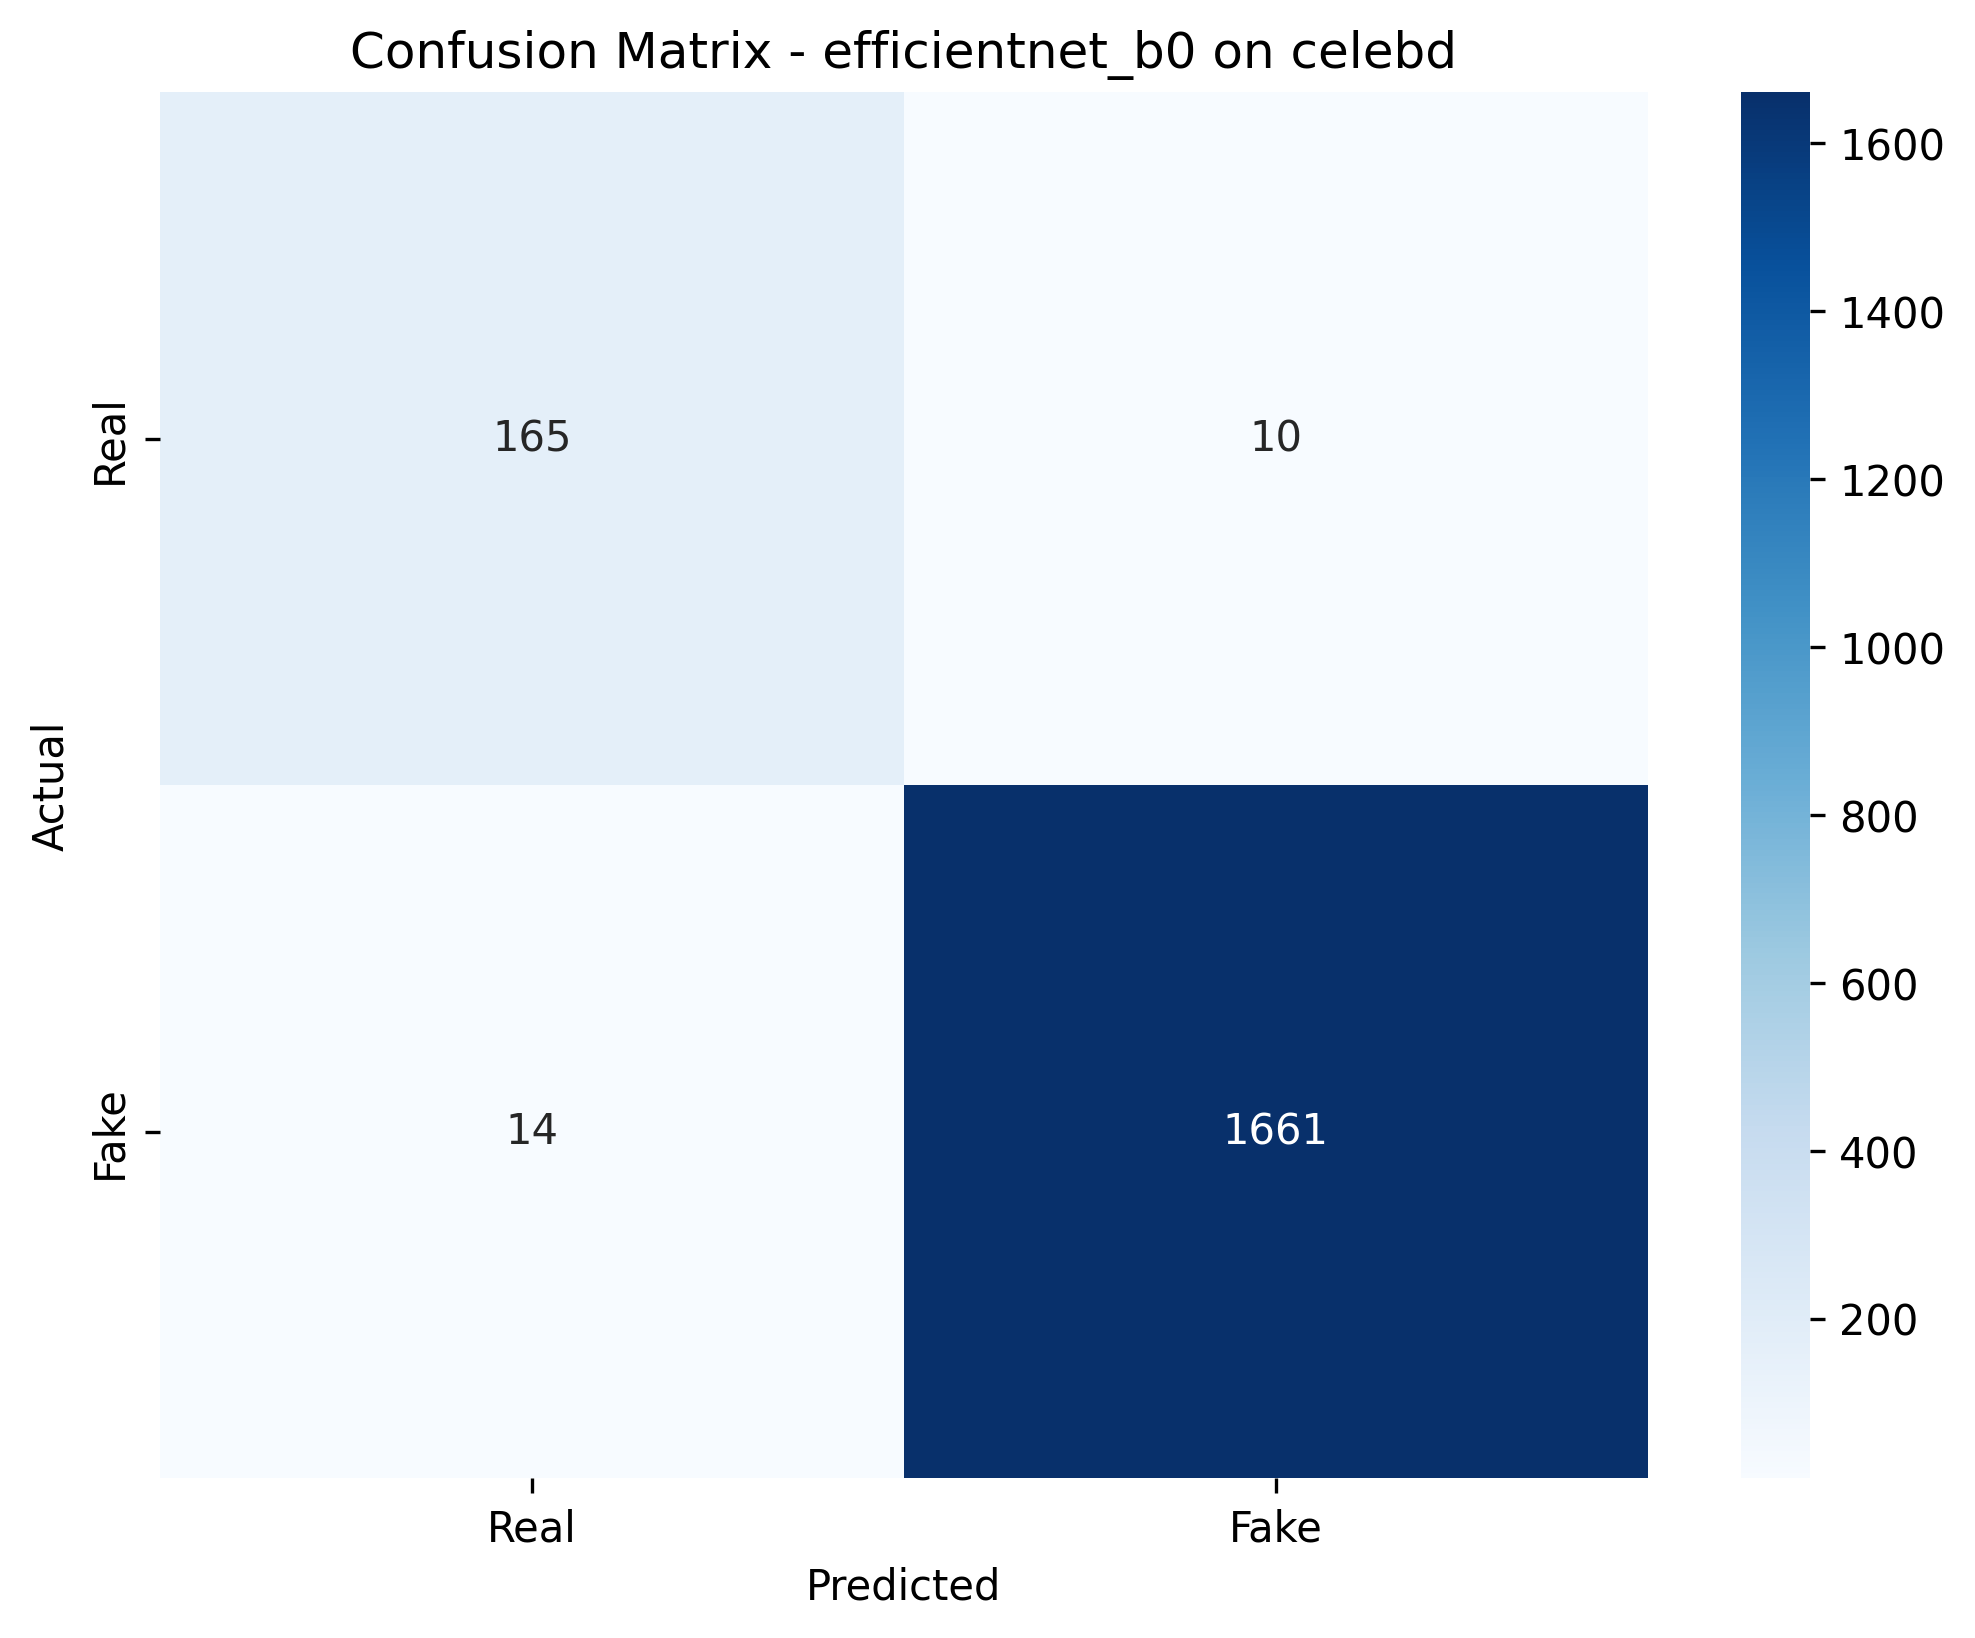
\includegraphics[width=0.20\textwidth]{figures/efficientnet_b0_celebd_confusion_matrix.png} &
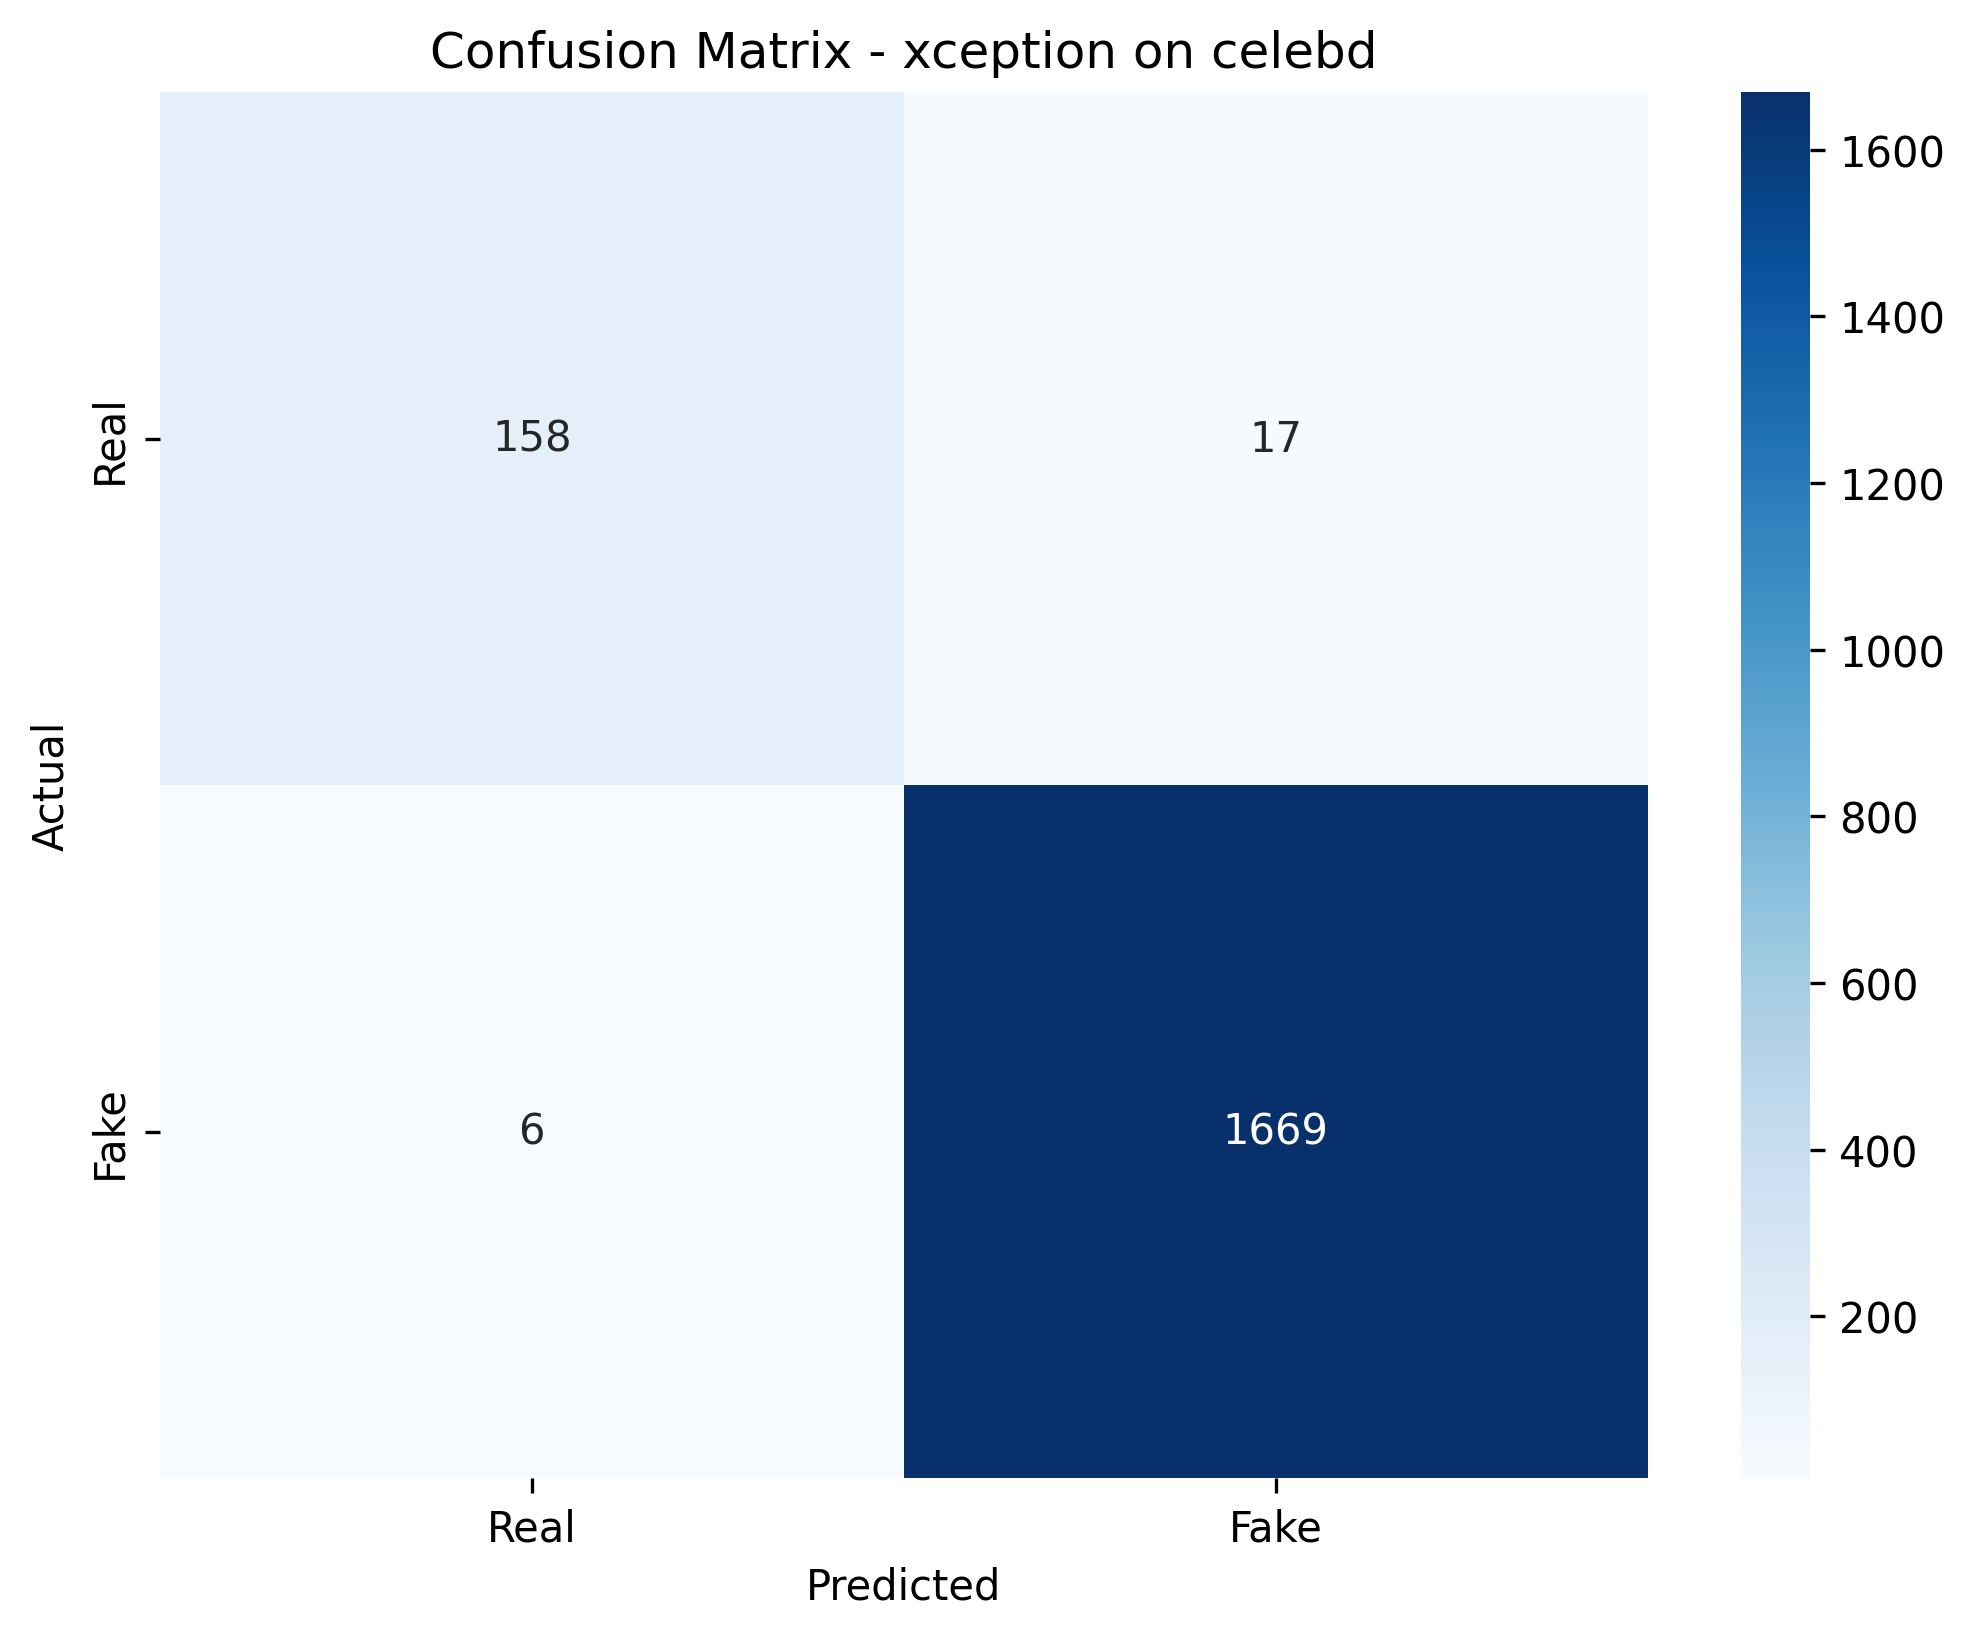
\includegraphics[width=0.20\textwidth]{figures/xception_celebd_confusion_matrix.png} \\
(a) EfficientNet-B0 & (b) XceptionNet \\
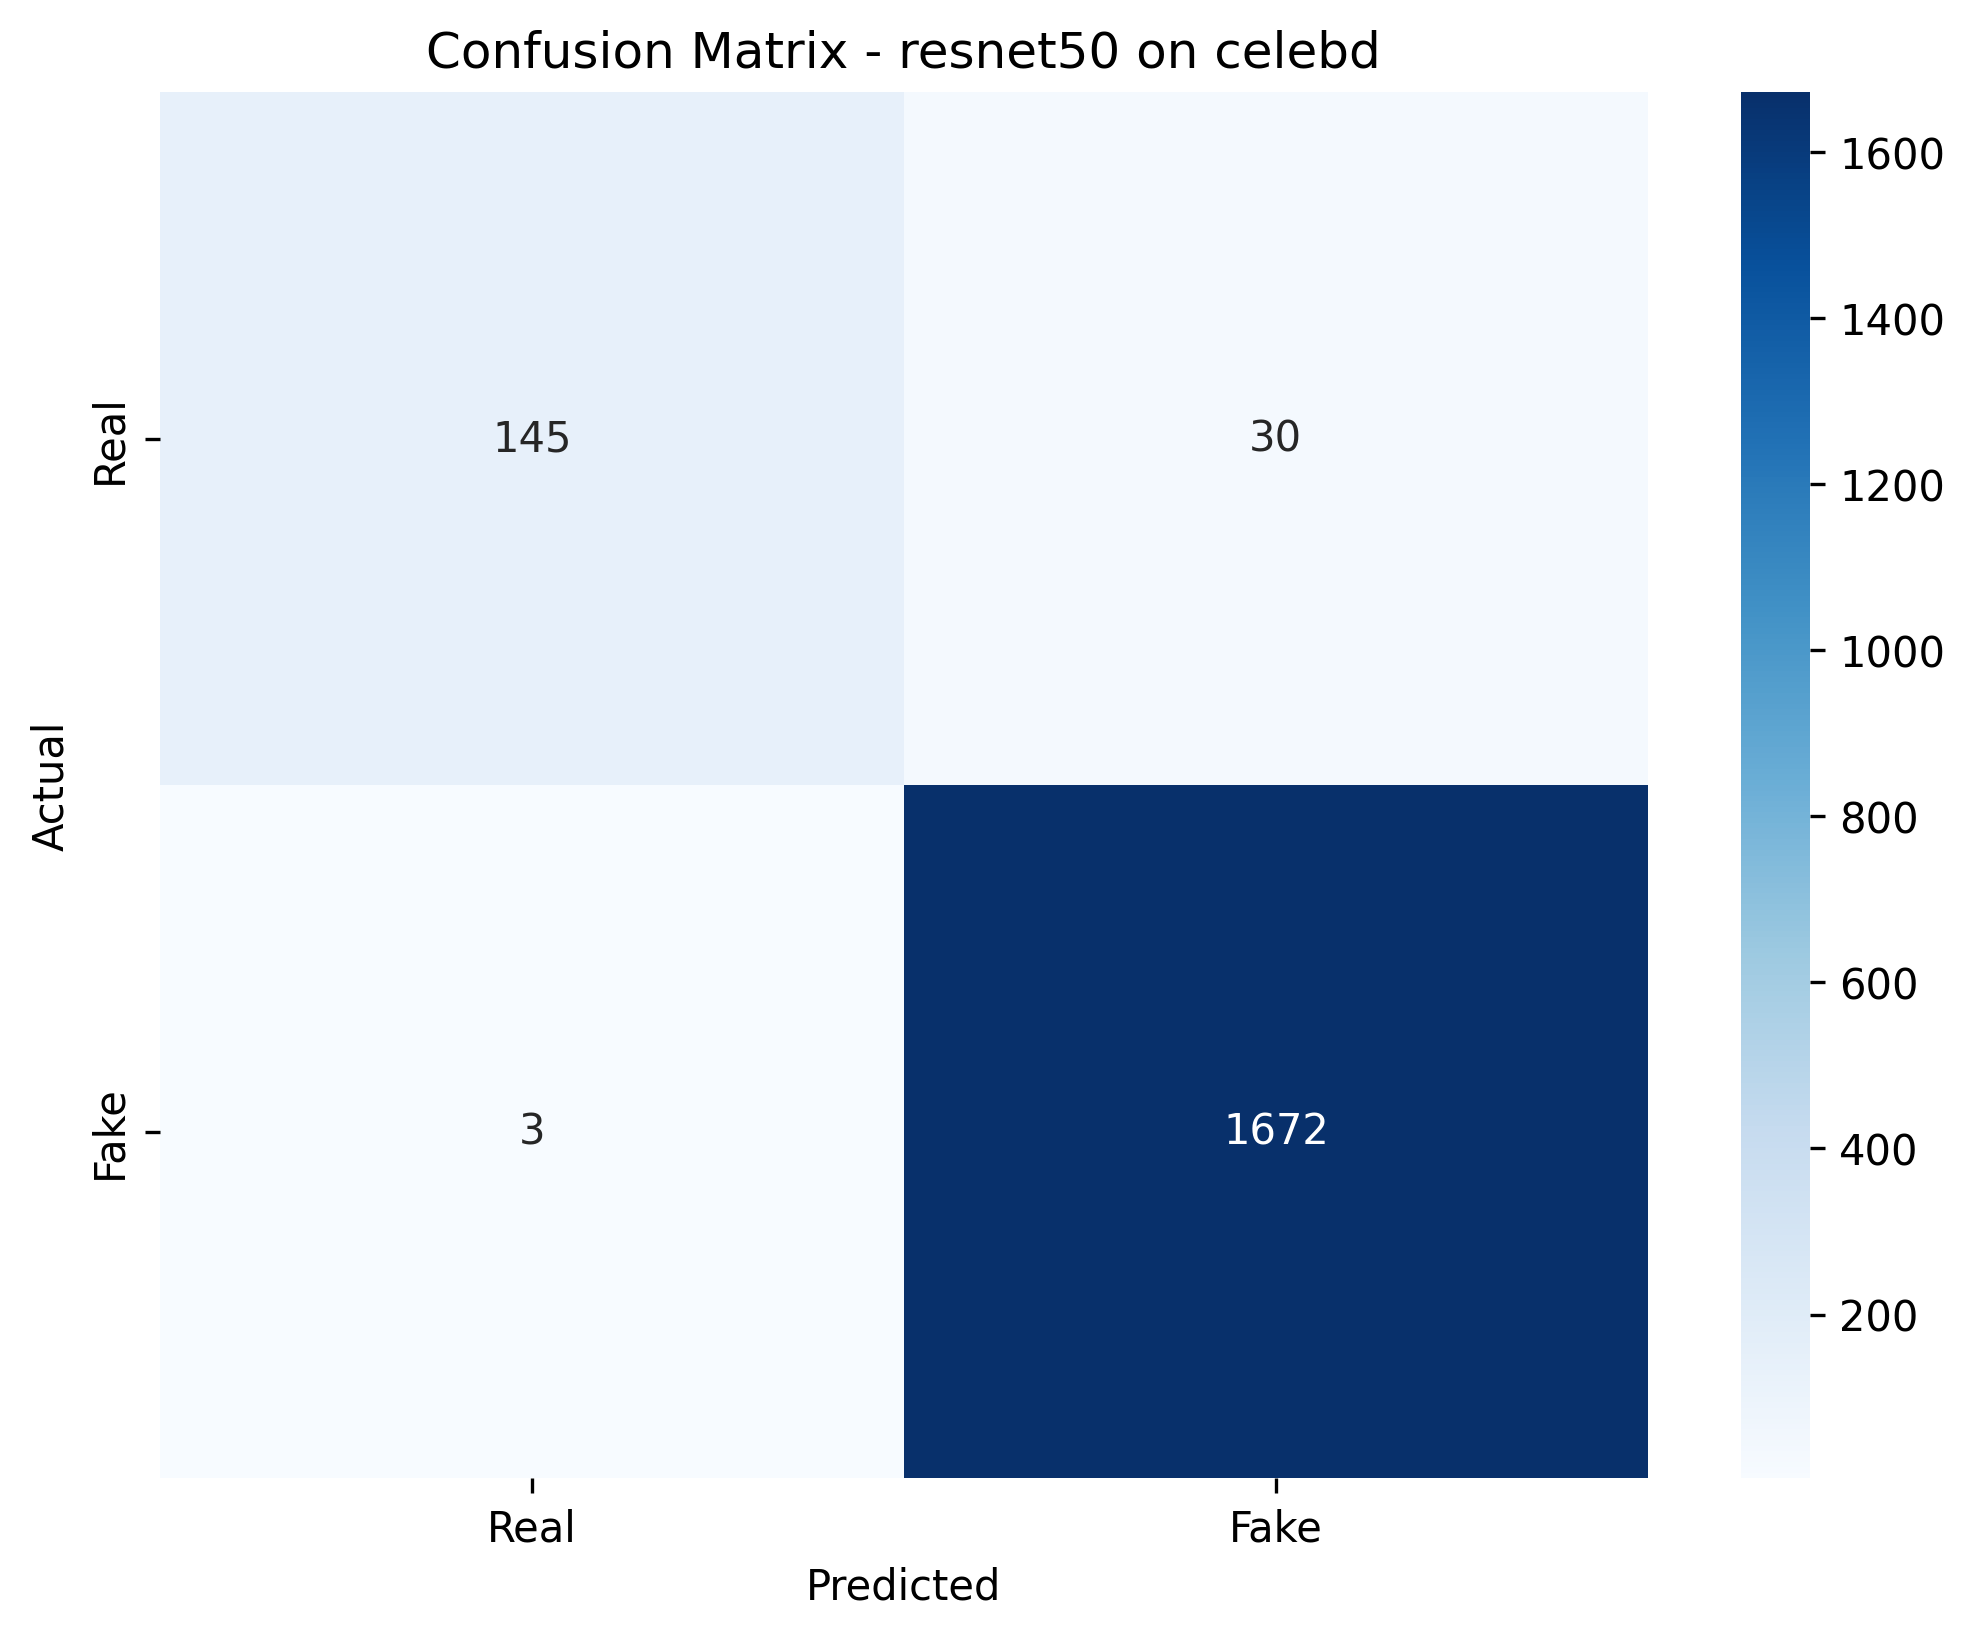
\includegraphics[width=0.20\textwidth]{figures/resnet50_celebd_confusion_matrix.png} &
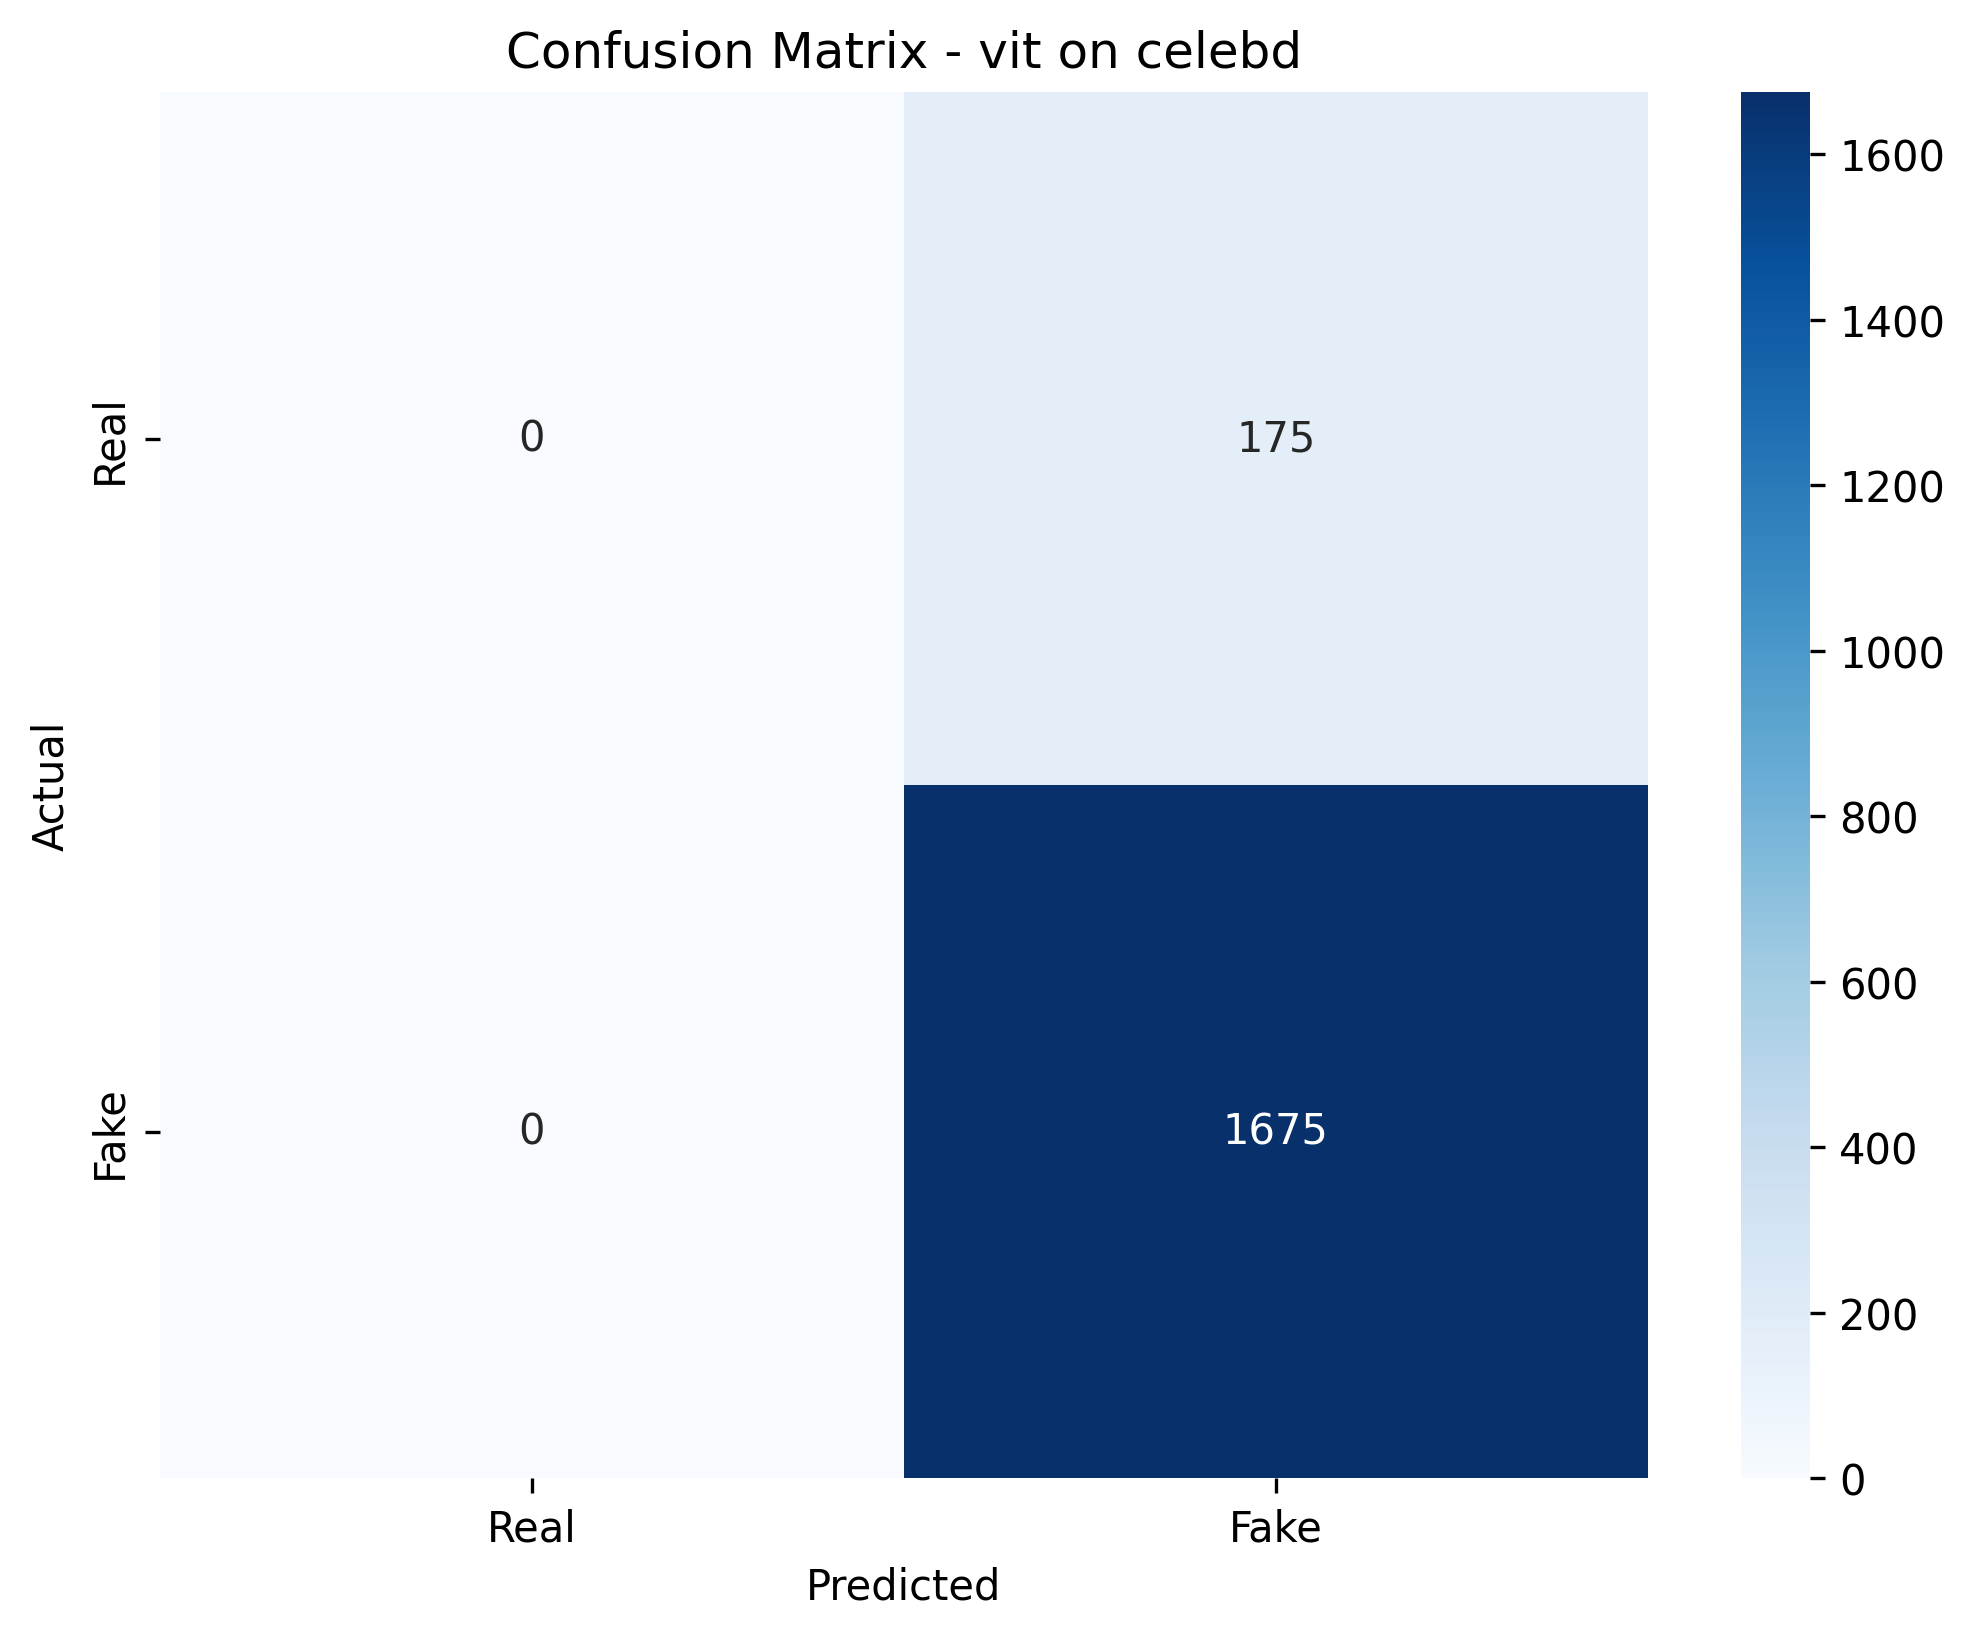
\includegraphics[width=0.20\textwidth]{figures/vit_celebd_confusion_matrix.png} \\
(c) ResNet50 & (d) Vision Transformer
\end{tabular}
\caption{Confusion matrices for all four models on Celeb-DF test set.}
\label{fig:confusion_celebd}
\end{figure*}

\begin{figure*}[!htbp]
\centering
\vspace{-15pt}
\begin{tabular}{@{}c@{\hspace{4pt}}c@{}}
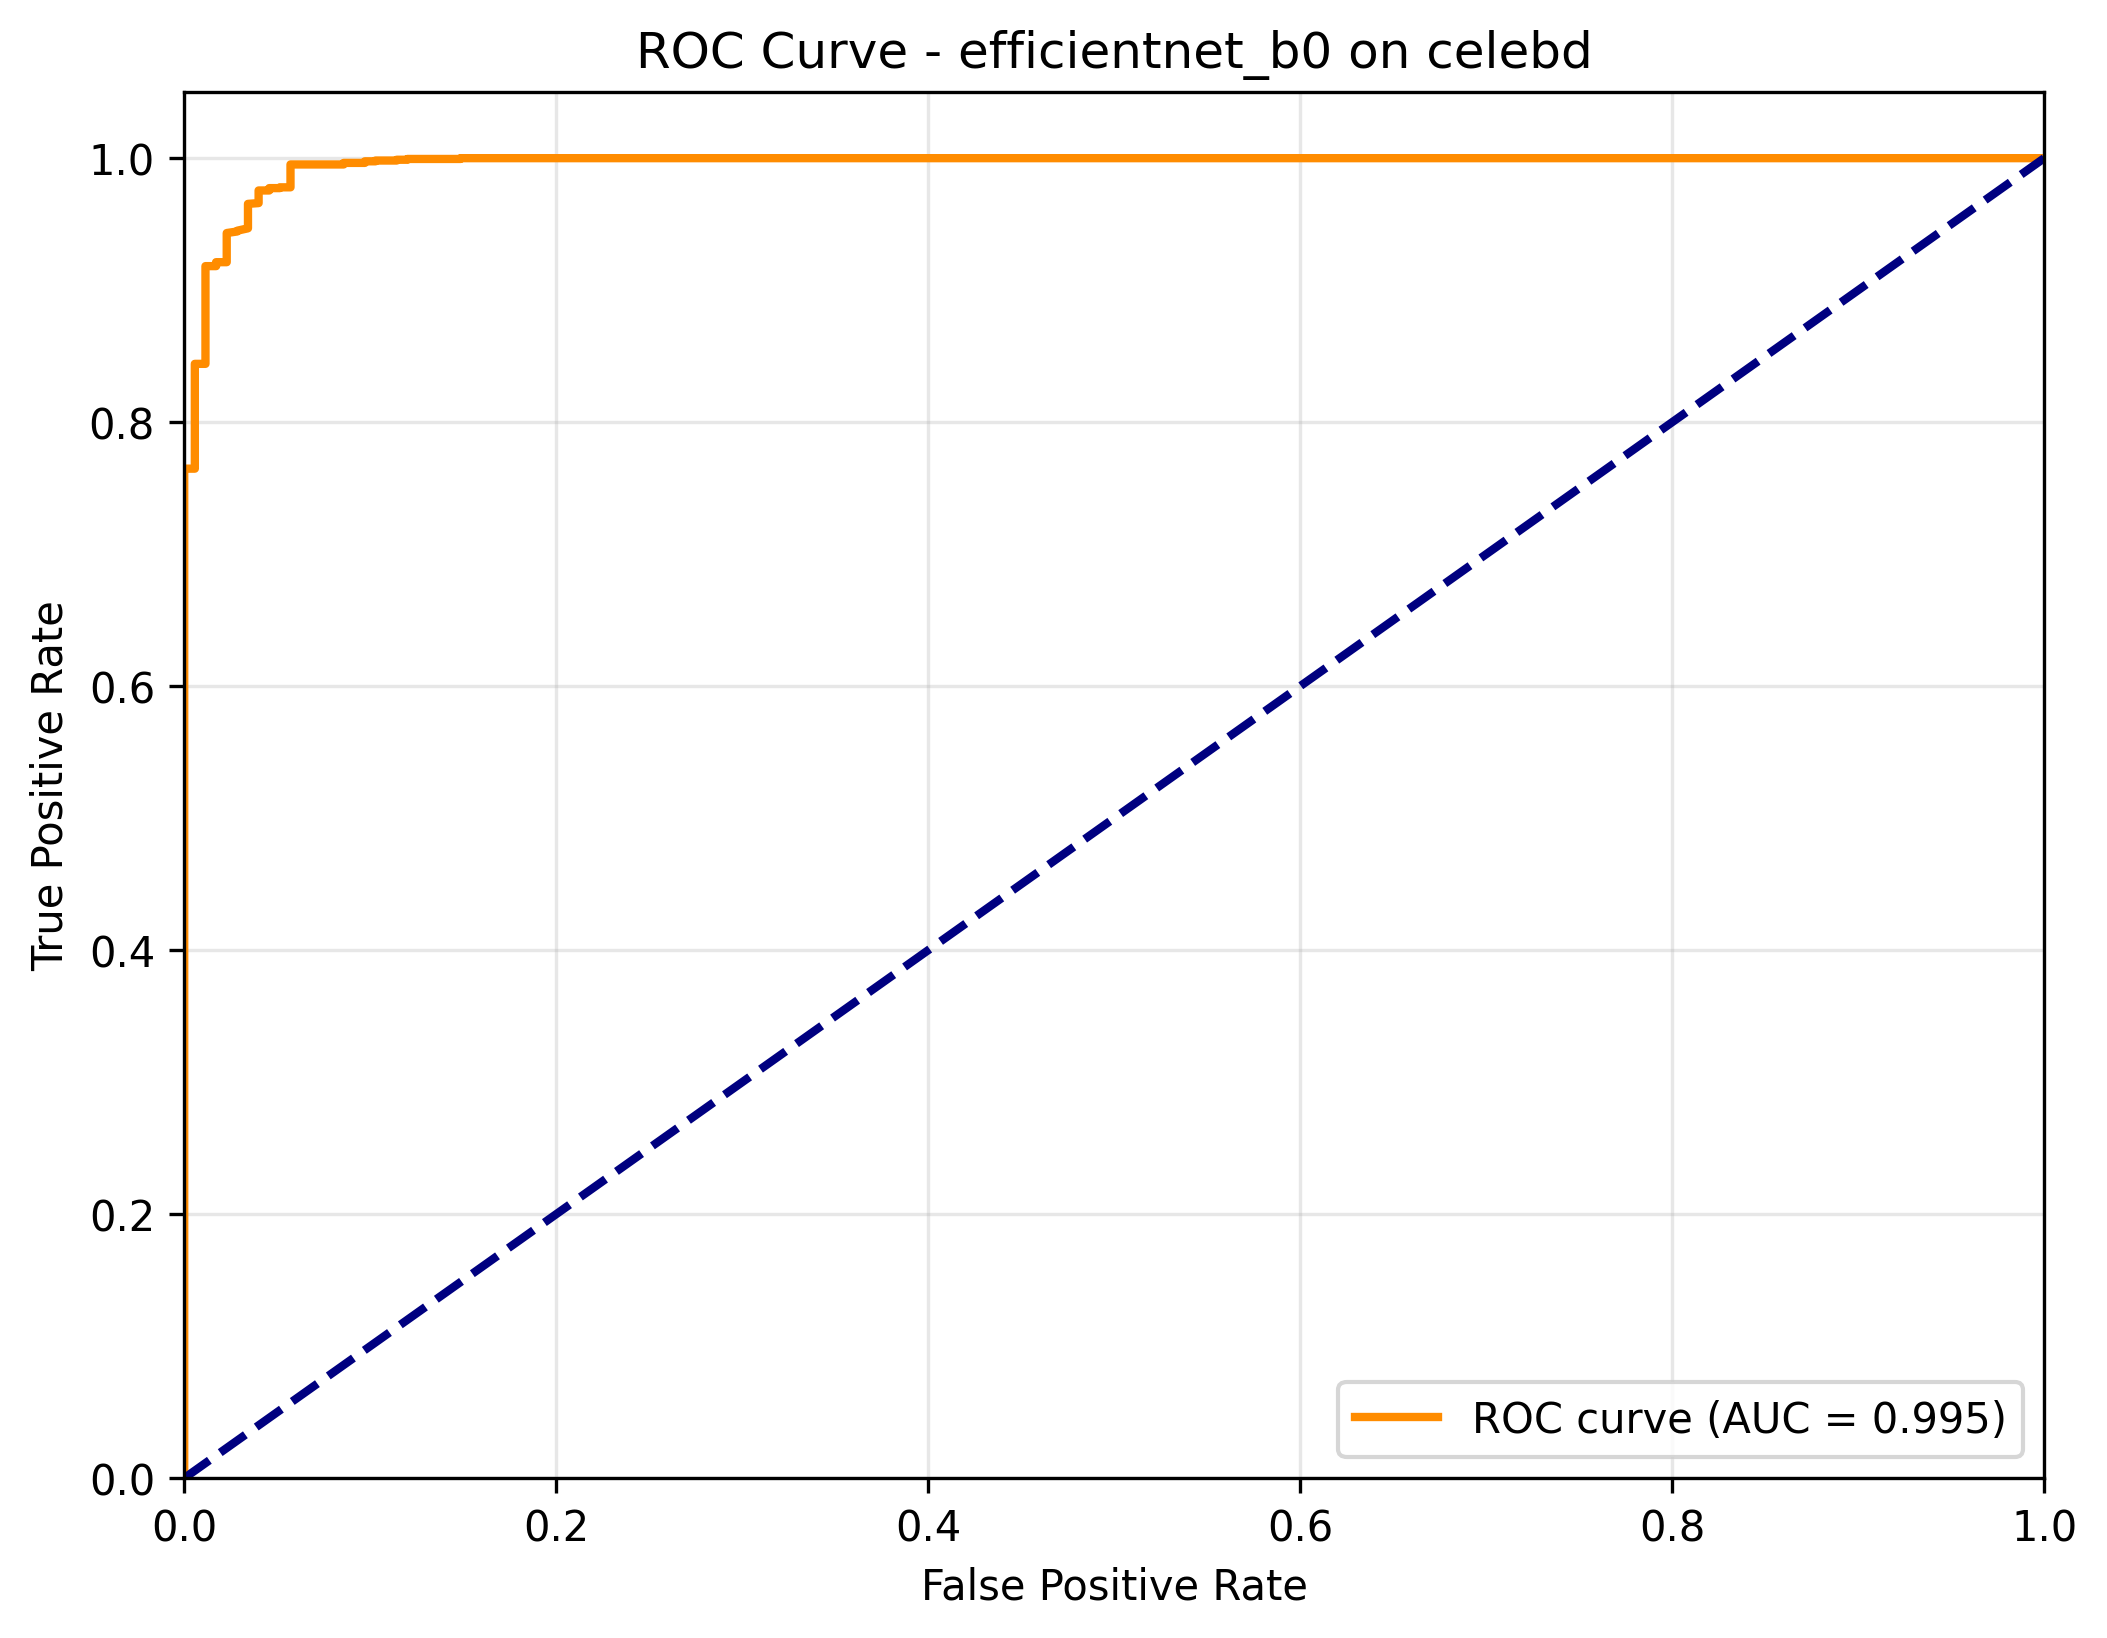
\includegraphics[width=0.19\textwidth]{figures/efficientnet_b0_celebd_roc_curve.png} &
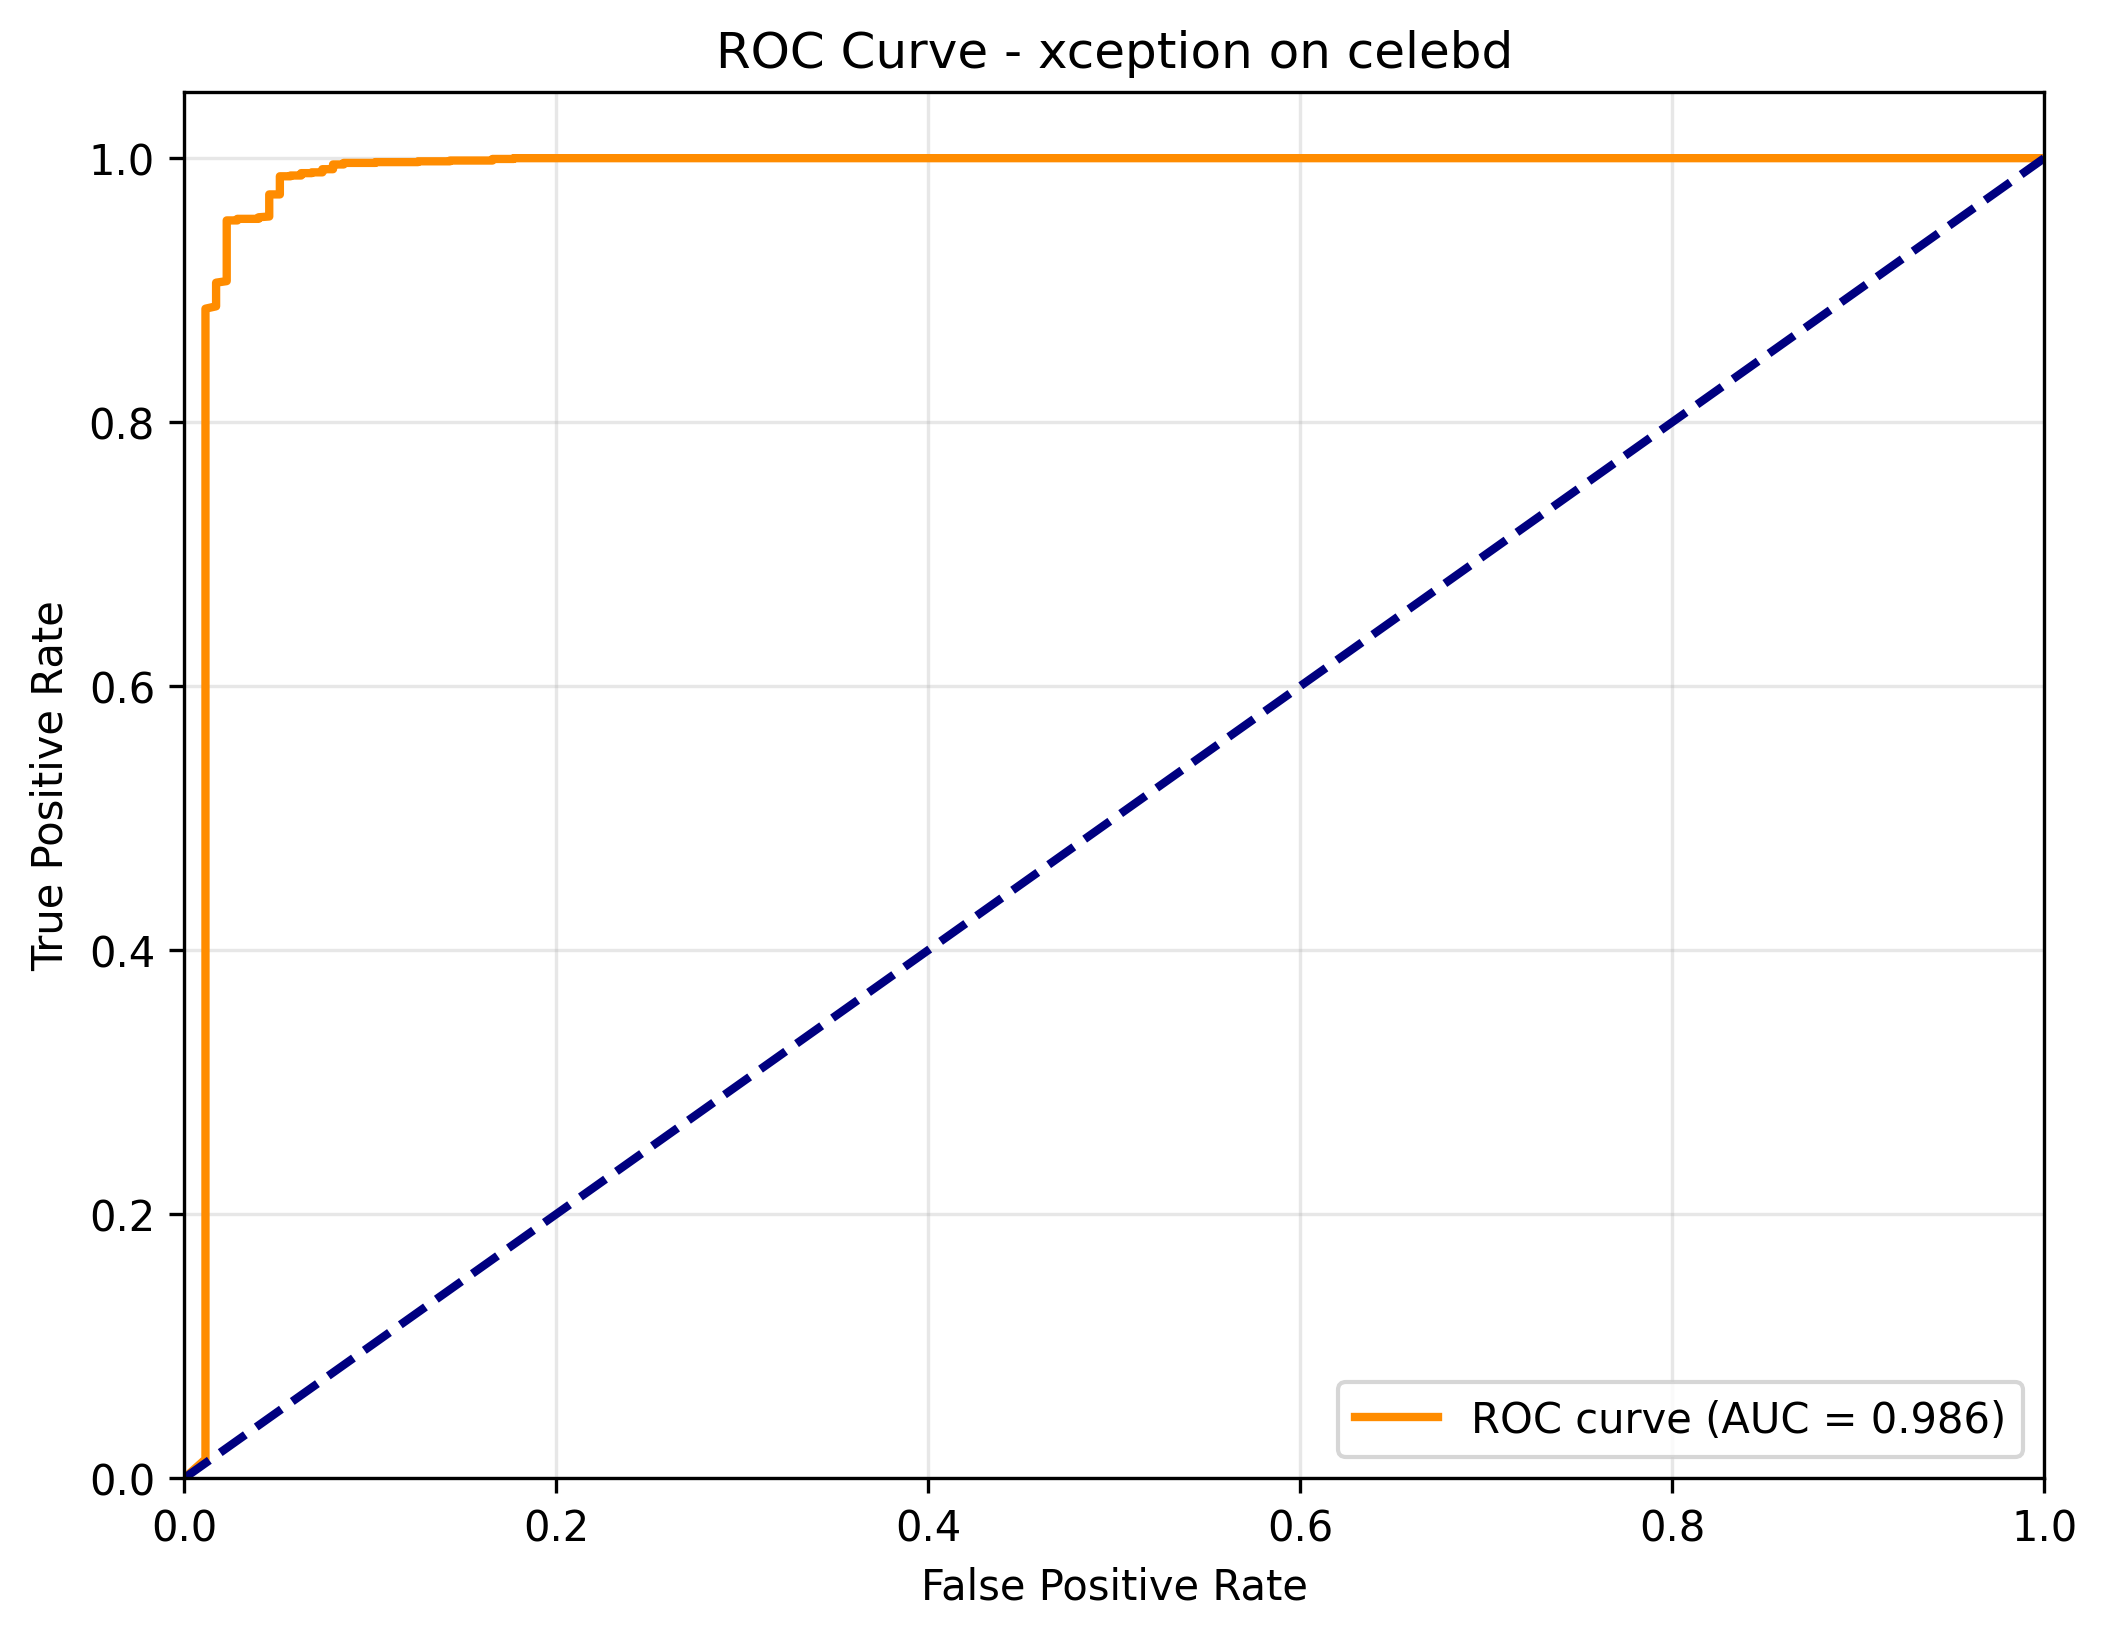
\includegraphics[width=0.19\textwidth]{figures/xception_celebd_roc_curve.png} \\
(a) EfficientNet-B0 & (b) XceptionNet \\[2pt]
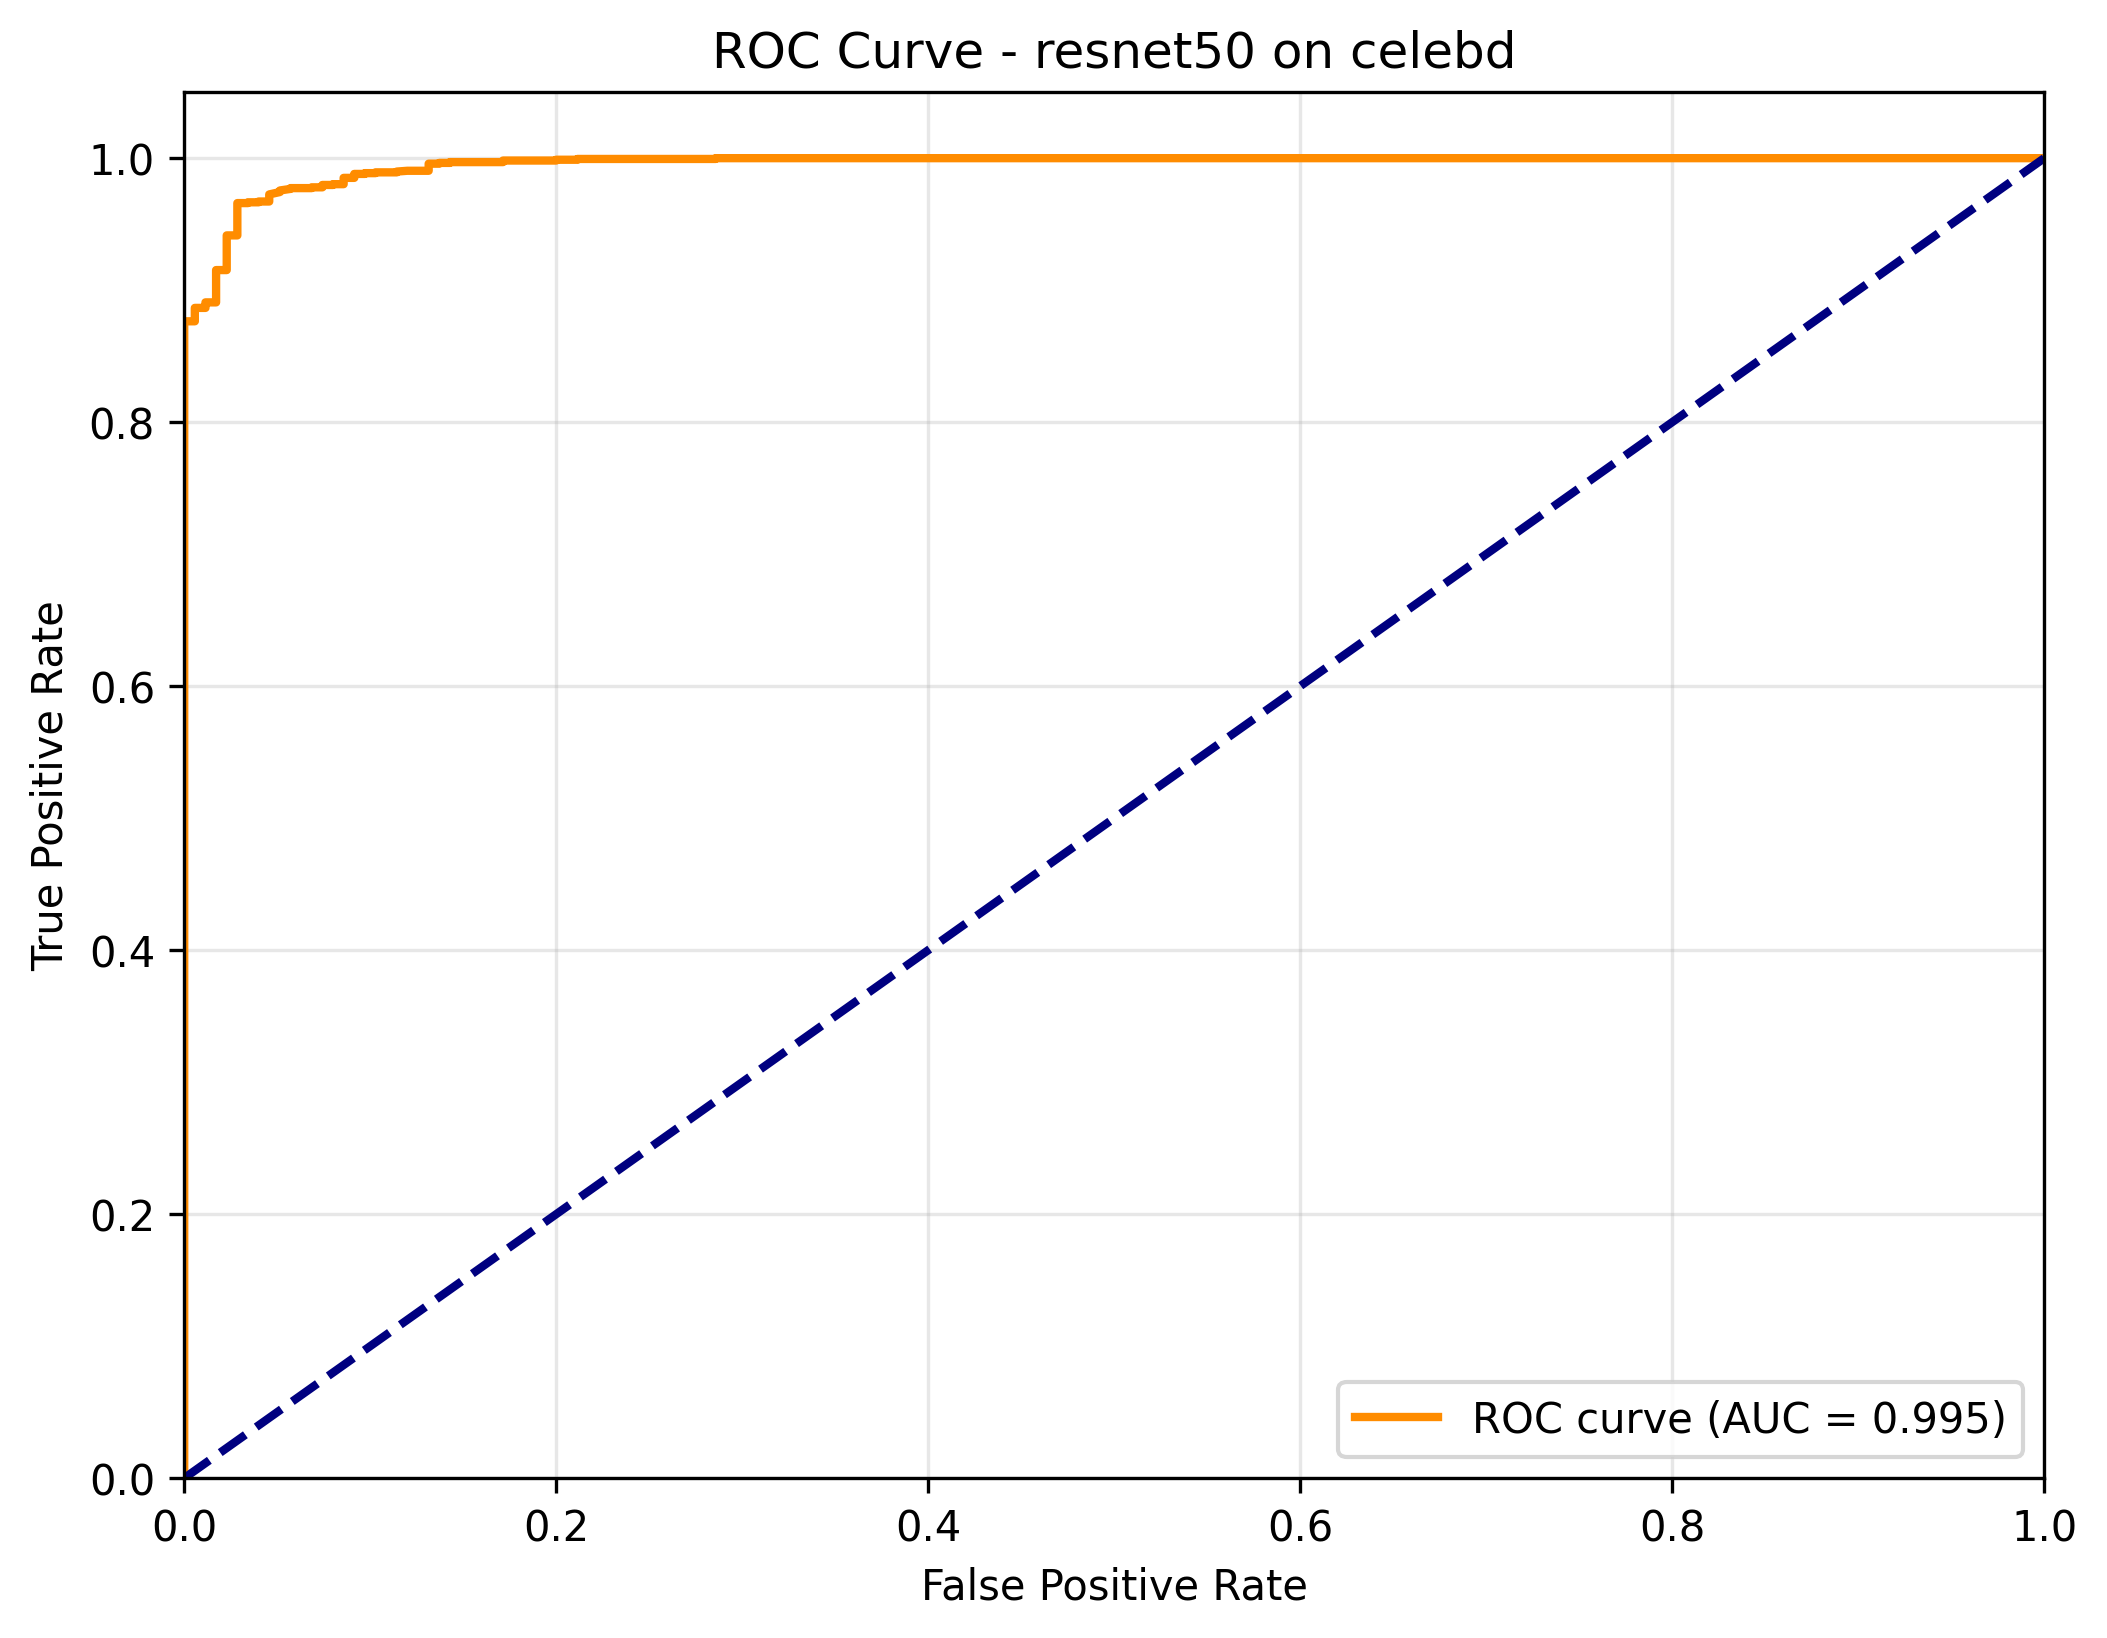
\includegraphics[width=0.19\textwidth]{figures/resnet50_celebd_roc_curve.png} &
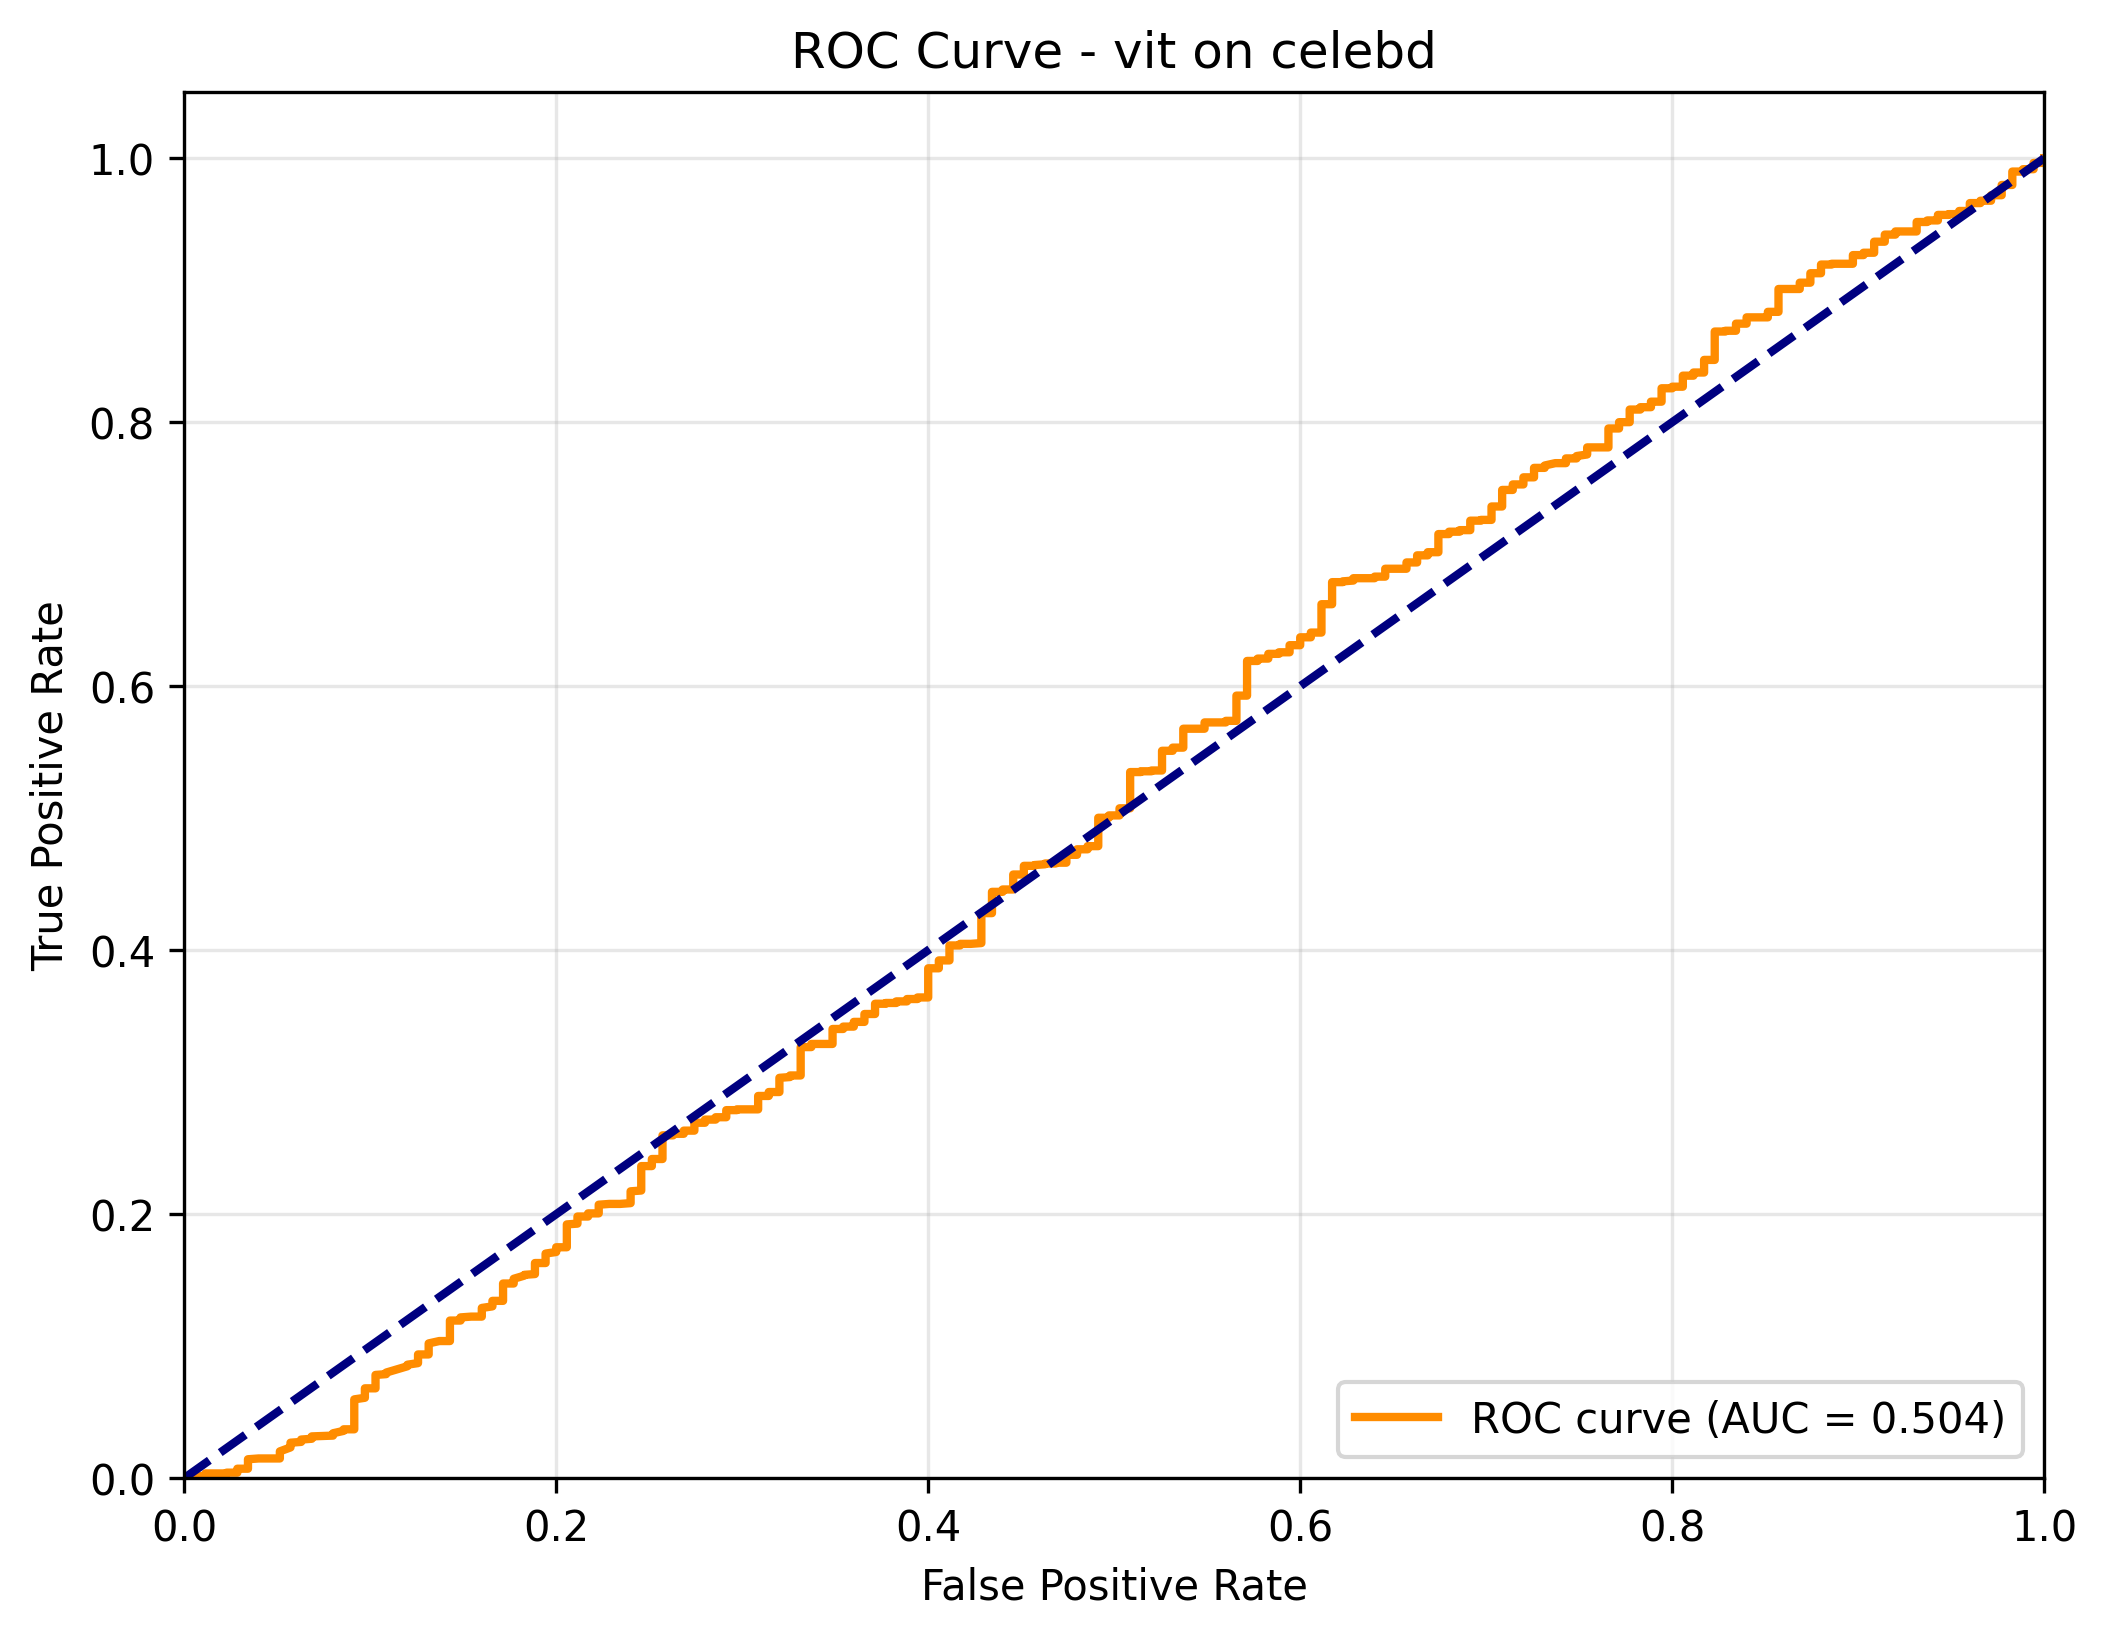
\includegraphics[width=0.19\textwidth]{figures/vit_celebd_roc_curve.png} \\
(c) ResNet50 & (d) Vision Transformer
\end{tabular}
\vspace{-2pt}
\caption{ROC curves for all four models on Celeb-DF test set.}
\label{fig:roc_celebd}

\vspace{4pt} % Tightened gap between figures

\begin{tabular}{@{}c@{\hspace{4pt}}c@{}}
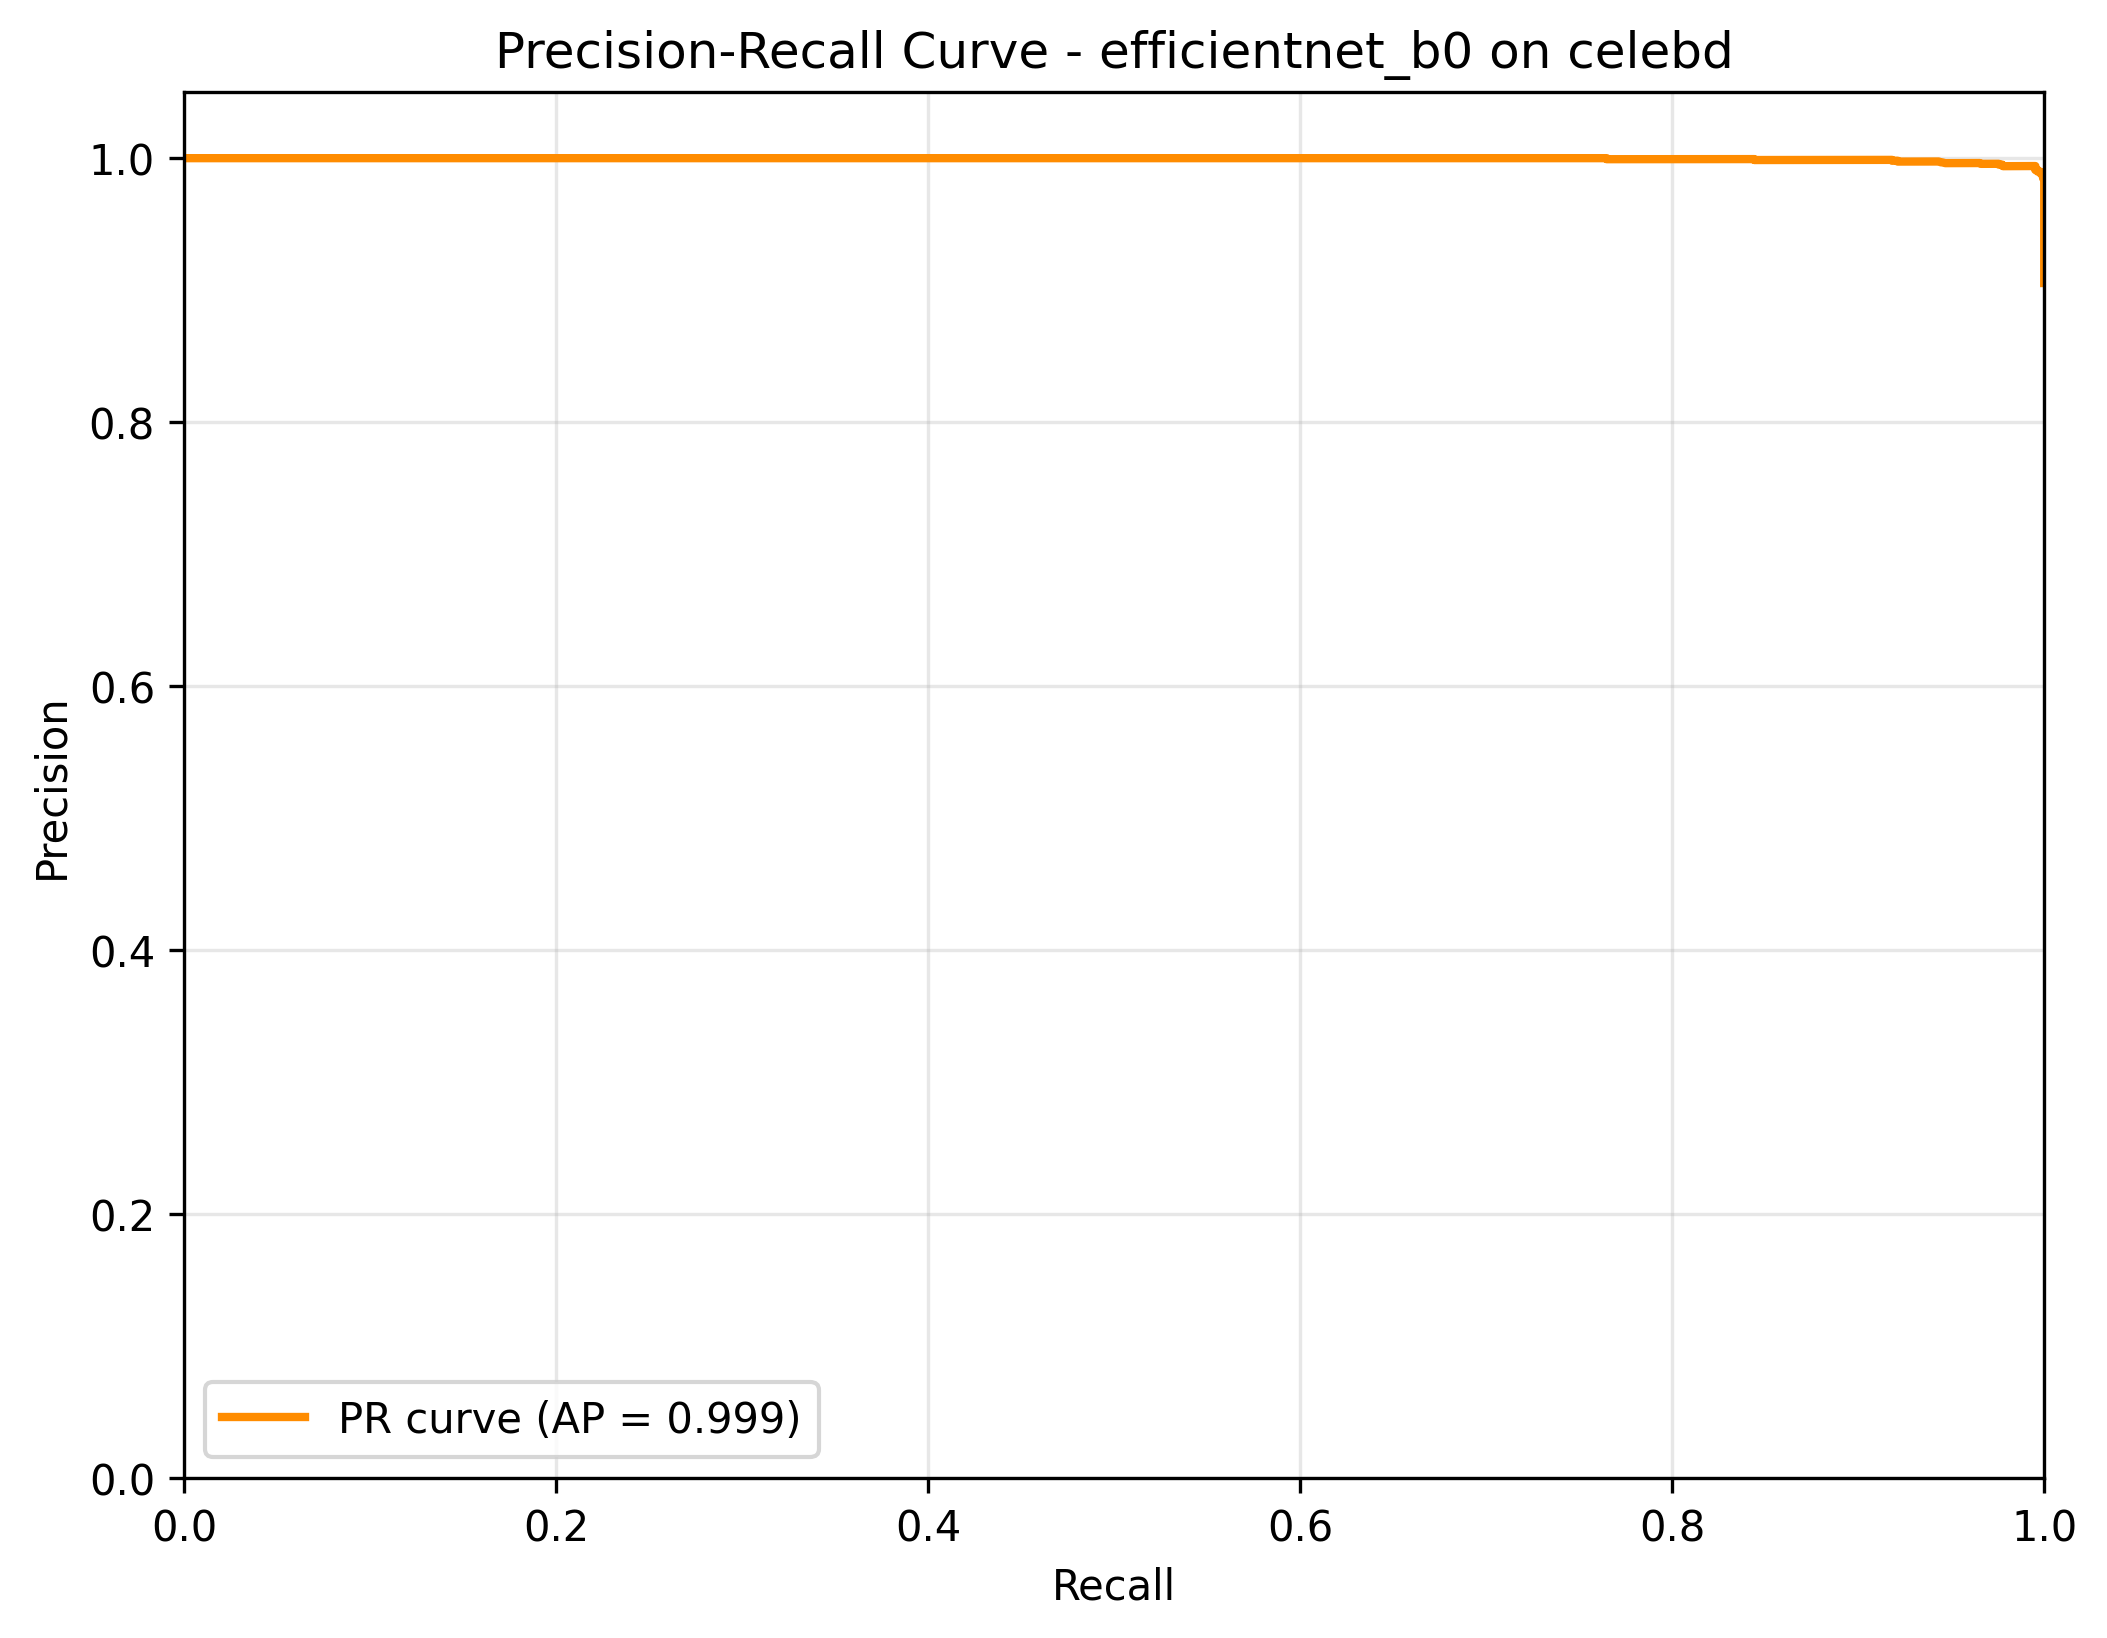
\includegraphics[width=0.19\textwidth]{figures/efficientnet_b0_celebd_precision_recall_curve.png} &
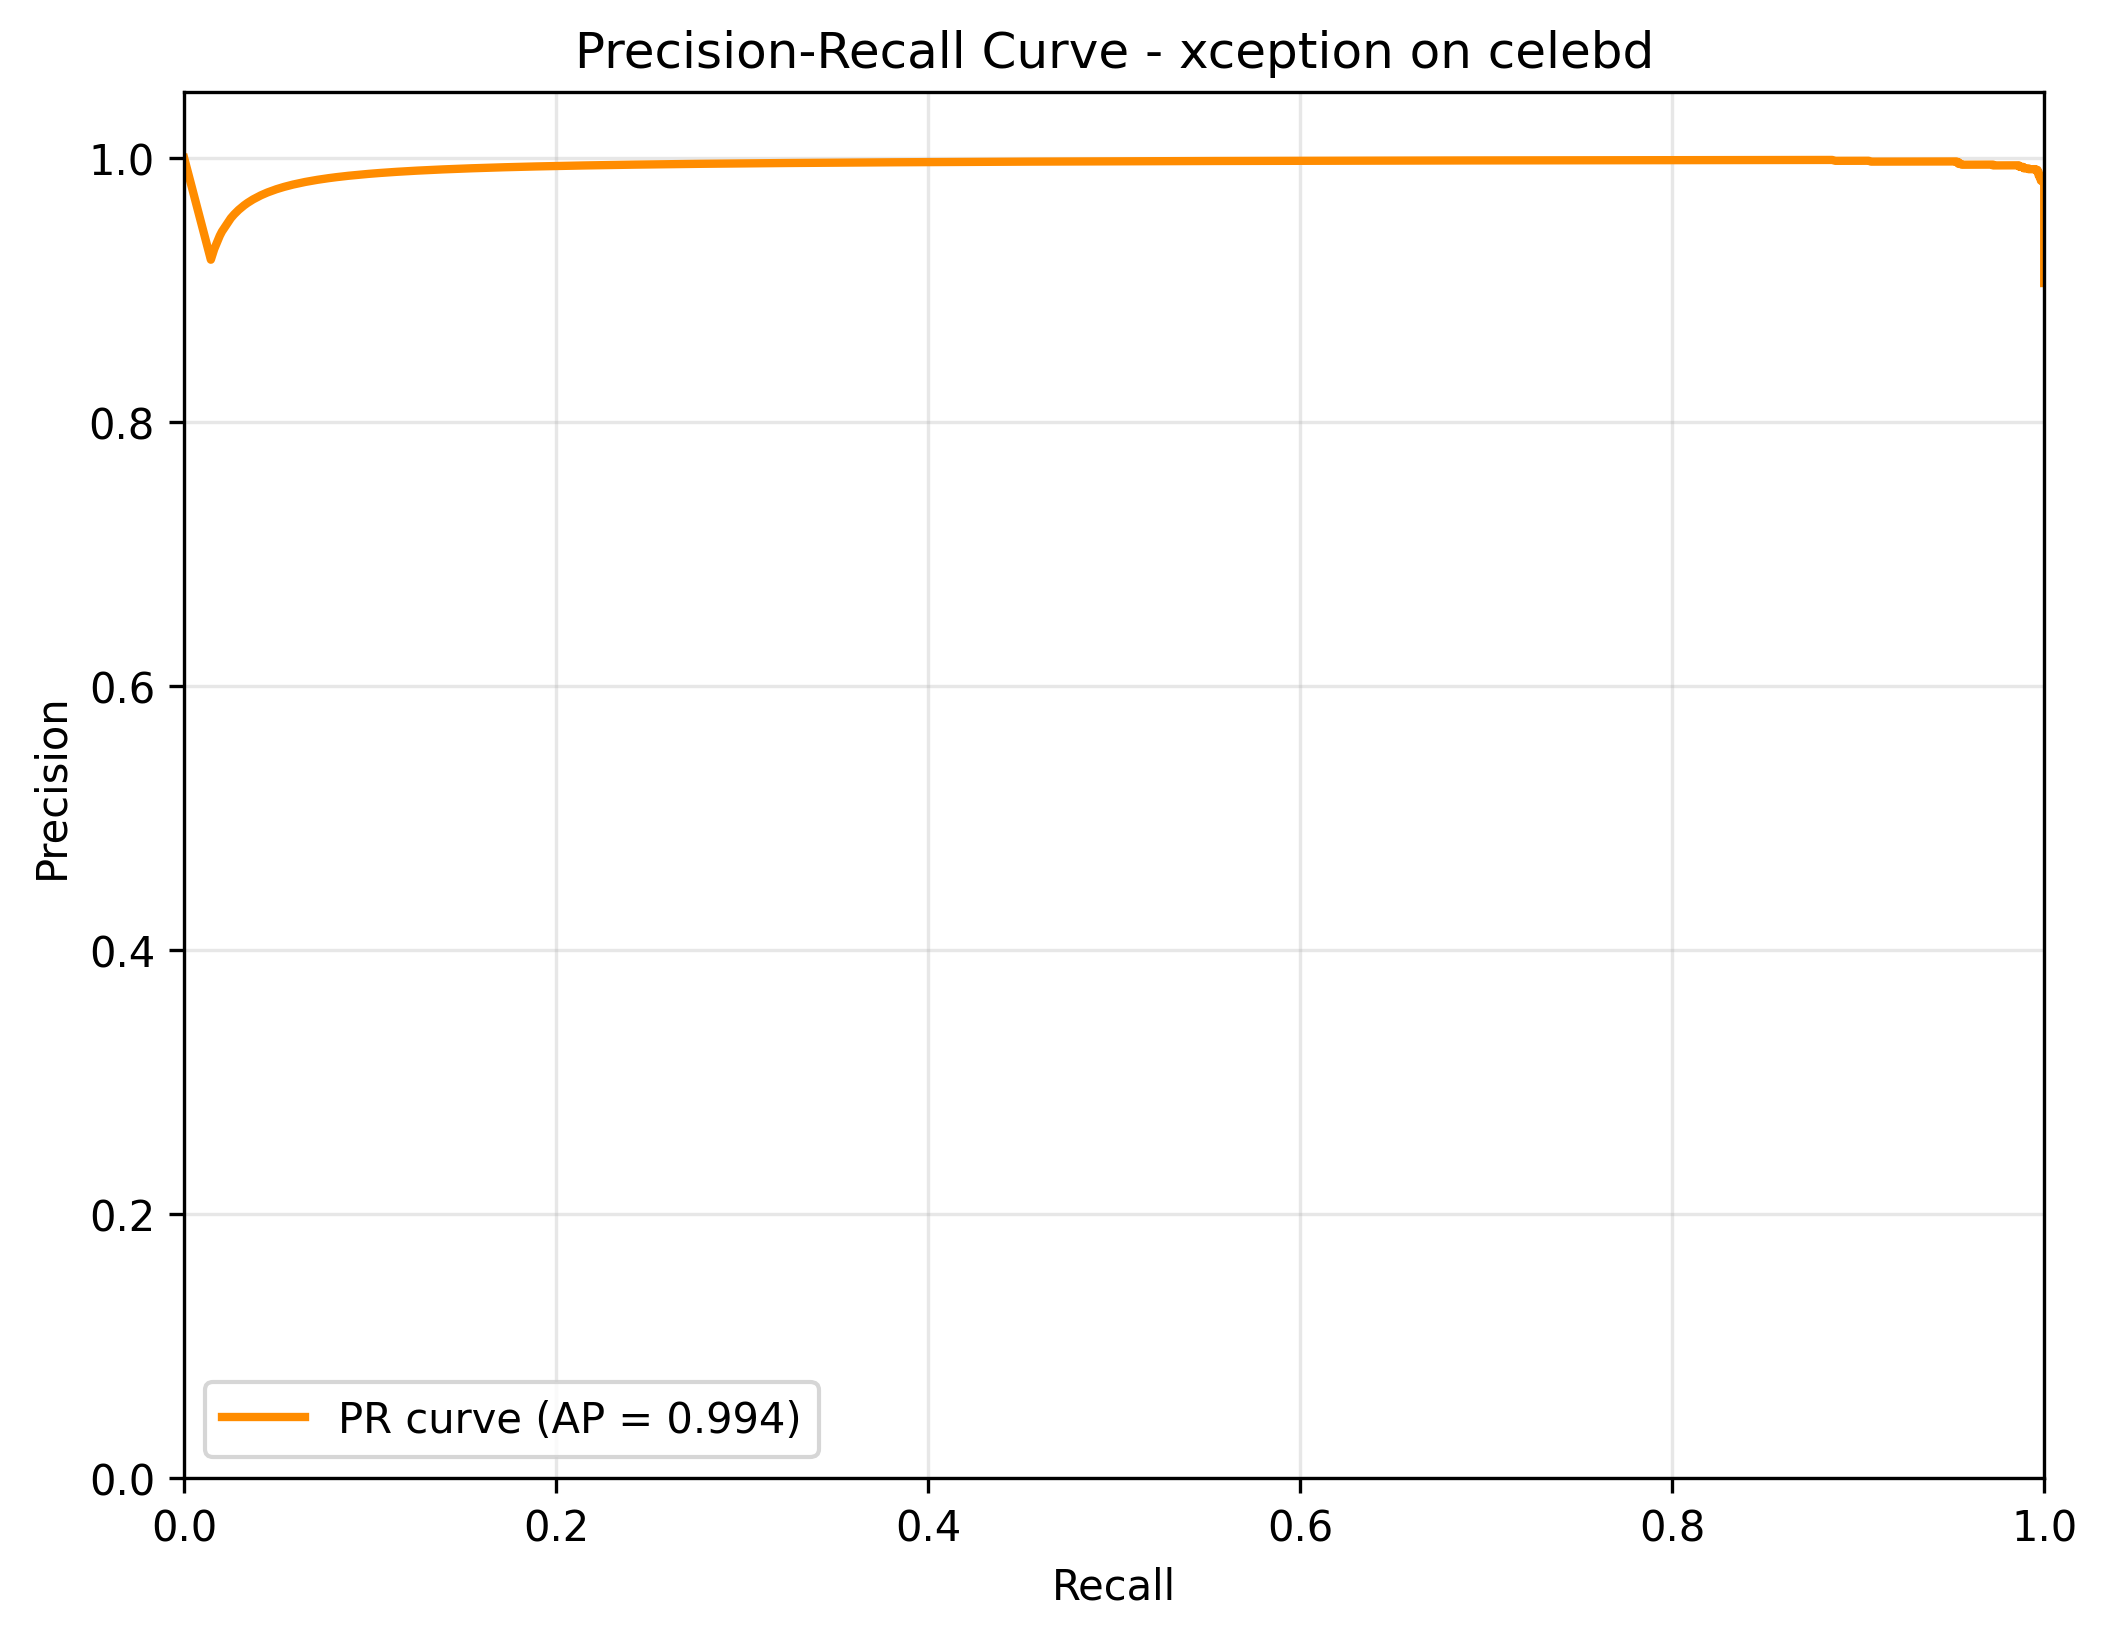
\includegraphics[width=0.19\textwidth]{figures/xception_celebd_precision_recall_curve.png} \\
(a) EfficientNet-B0 & (b) XceptionNet \\[2pt]
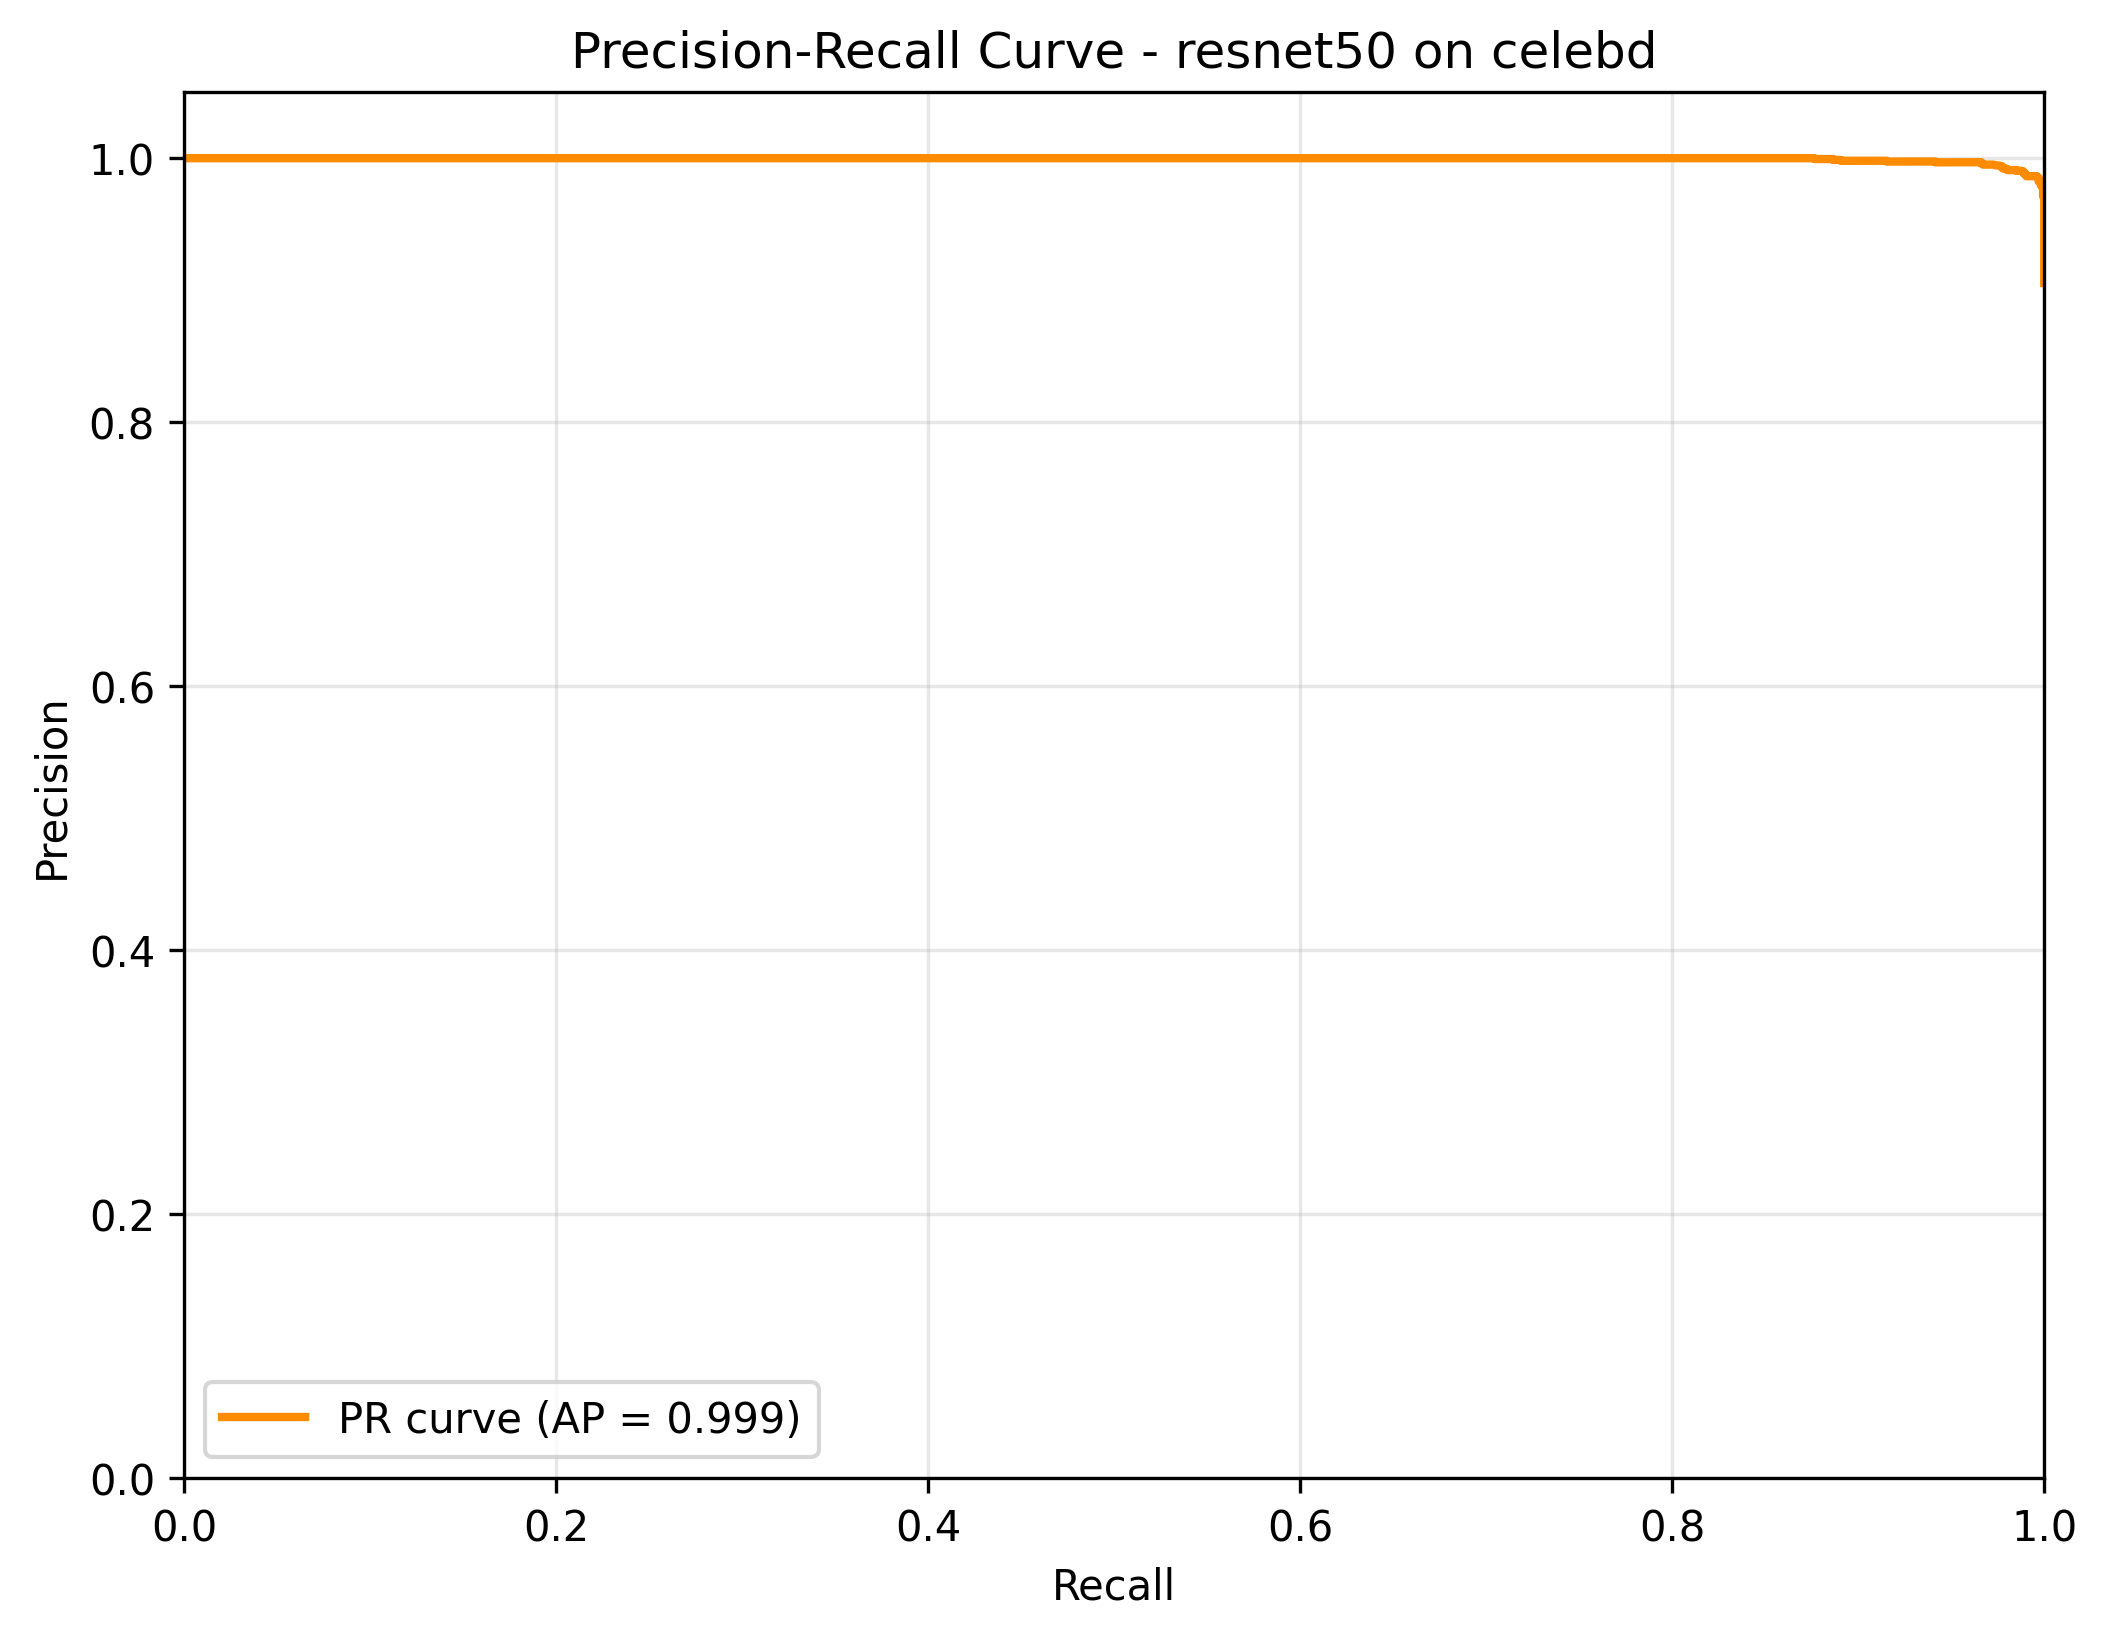
\includegraphics[width=0.19\textwidth]{figures/resnet50_celebd_precision_recall_curve.png} &
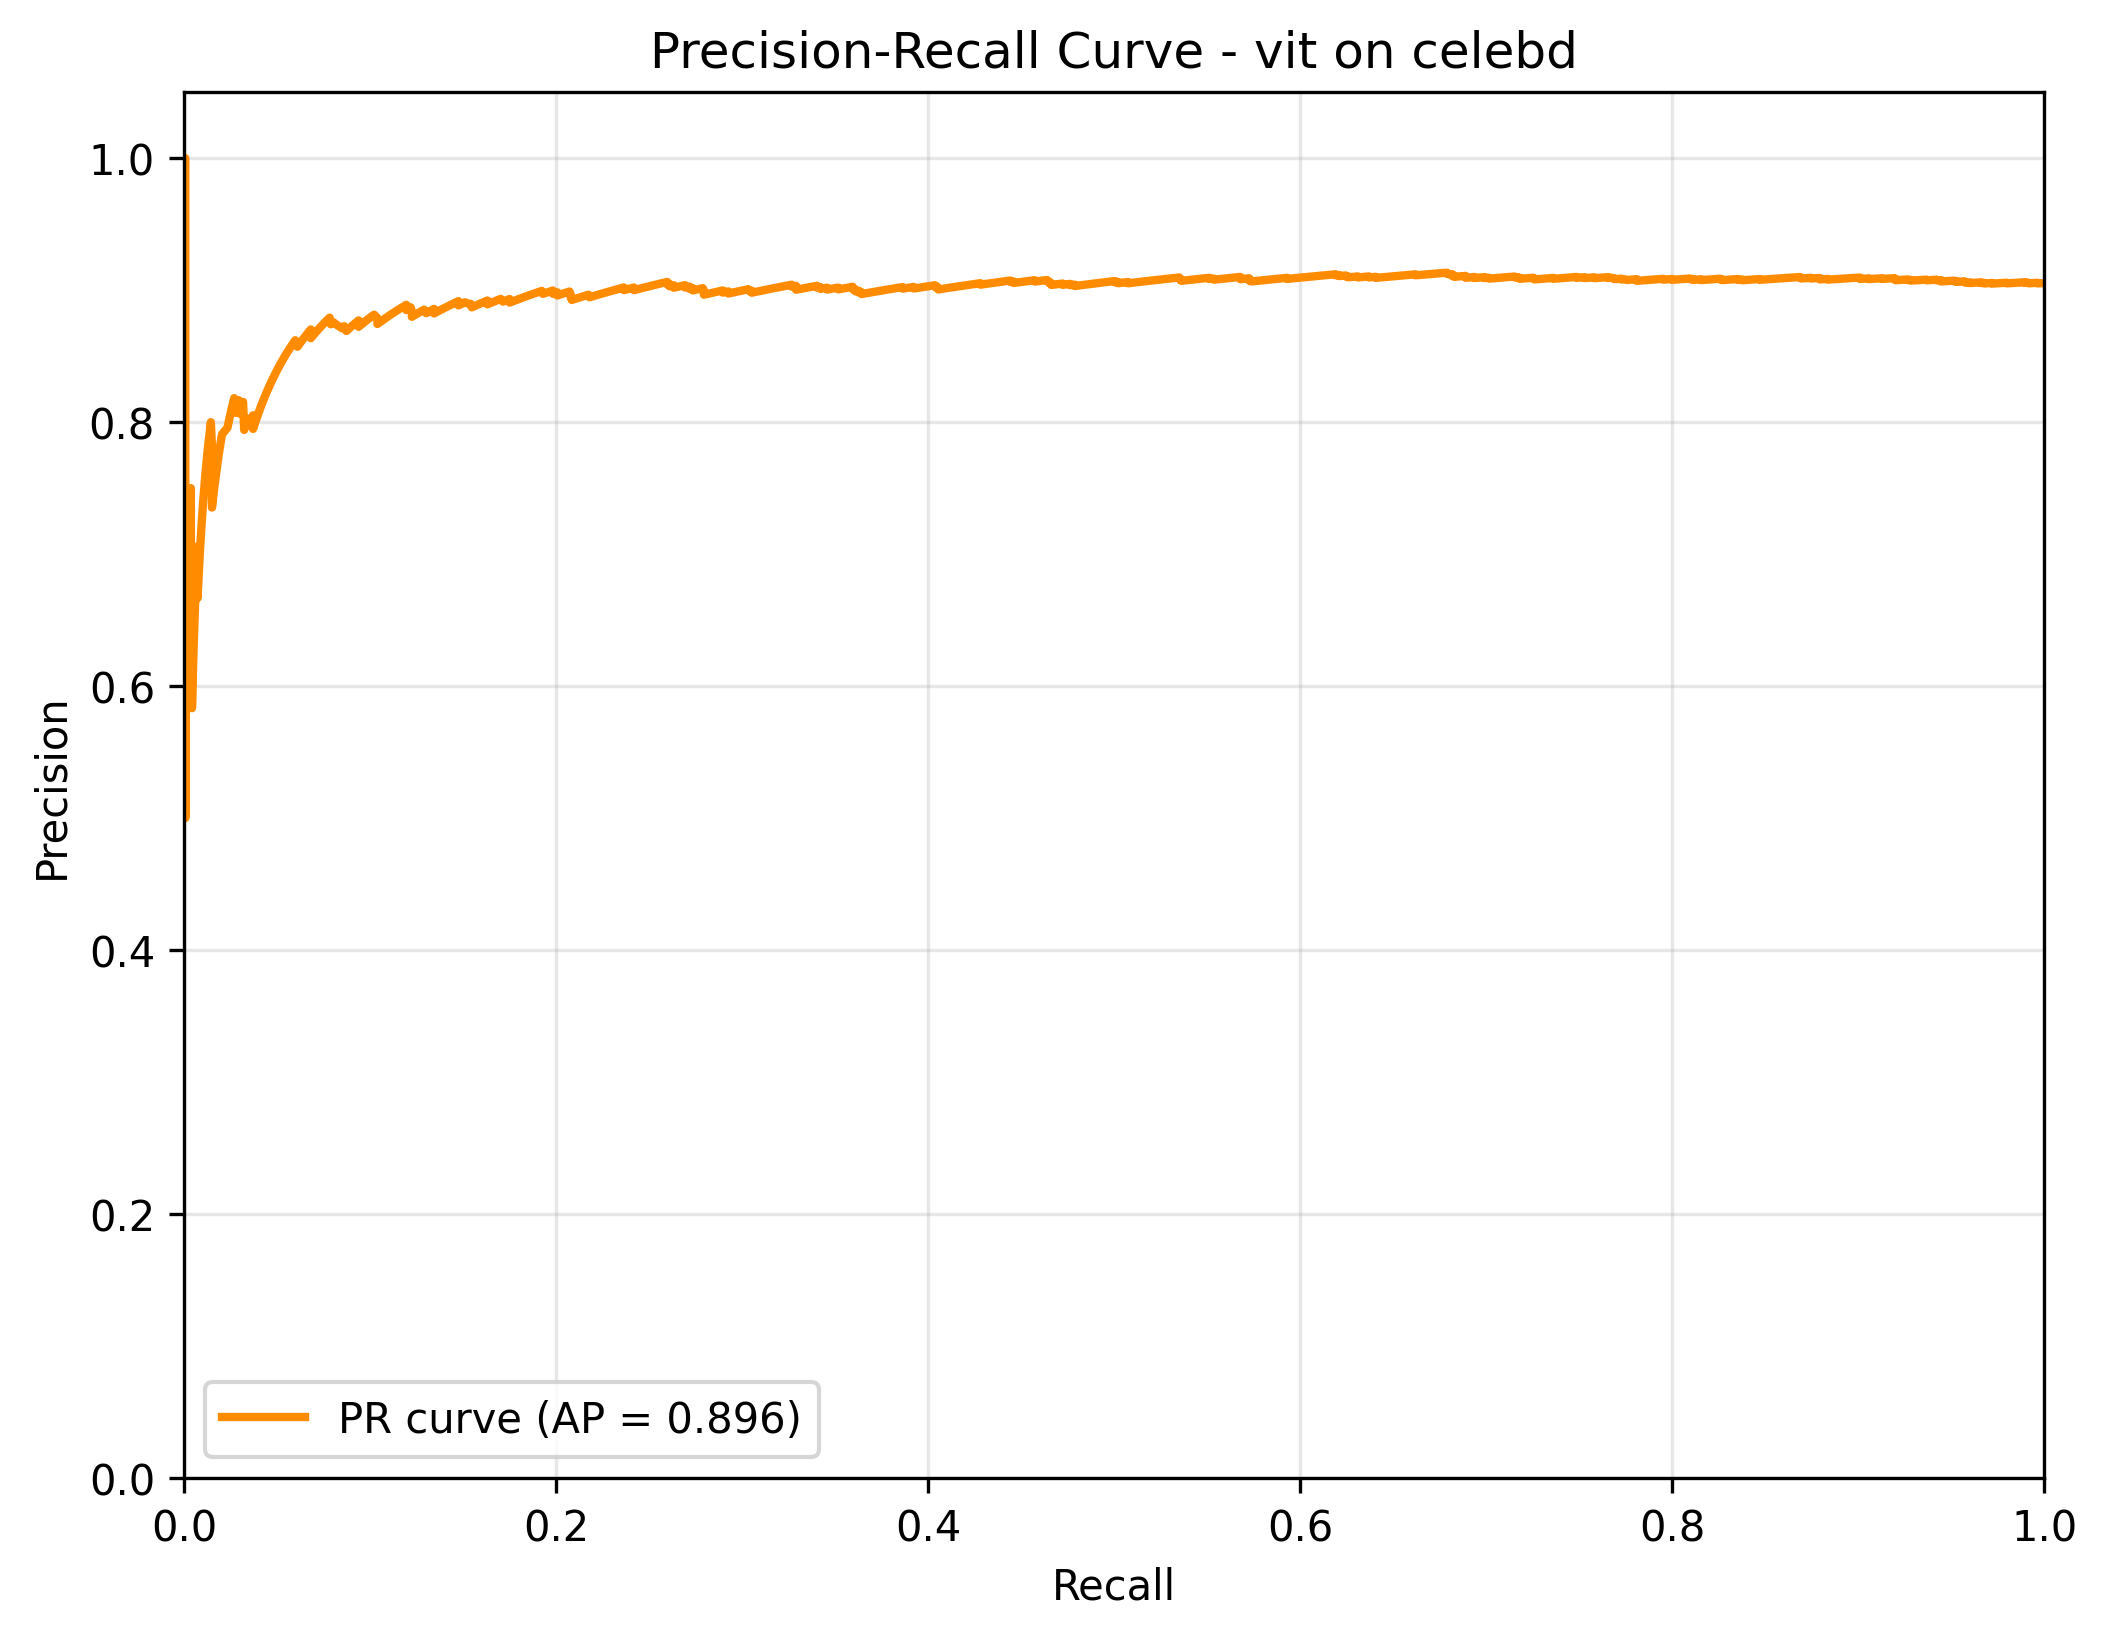
\includegraphics[width=0.19\textwidth]{figures/vit_celebd_precision_recall_curve.png} \\
(c) ResNet50 & (d) Vision Transformer
\end{tabular}
\vspace{-2pt}
\caption{Precision-Recall curves for all four models on Celeb-DF test set.}
\label{fig:pr_celebd}
\vspace{-6pt}
\end{figure*}

The confusion matrices in Figure~\ref{fig:confusion_celebd} show that the CNN models make very few mistakes on familiar data, with strong diagonal dominance. The Vision Transformer, however, shows more false positives, which aligns with its lower precision of 81.98\%. The ROC curves in Figure~\ref{fig:roc_celebd} confirm this --- the CNN curves stay close to the top-left corner with AUC values above 98\%, while the ViT's curve is closer to the diagonal, reflecting its AUC of 50.35\%. The Precision-Recall curves in Figure~\ref{fig:pr_celebd} further confirm that the CNNs maintain high precision across different recall values on this dataset.

\subsection{Cross-Dataset Visualization}
\FloatBarrier

\begin{figure*}[!htbp]
\centering
\begin{tabular}{cc}
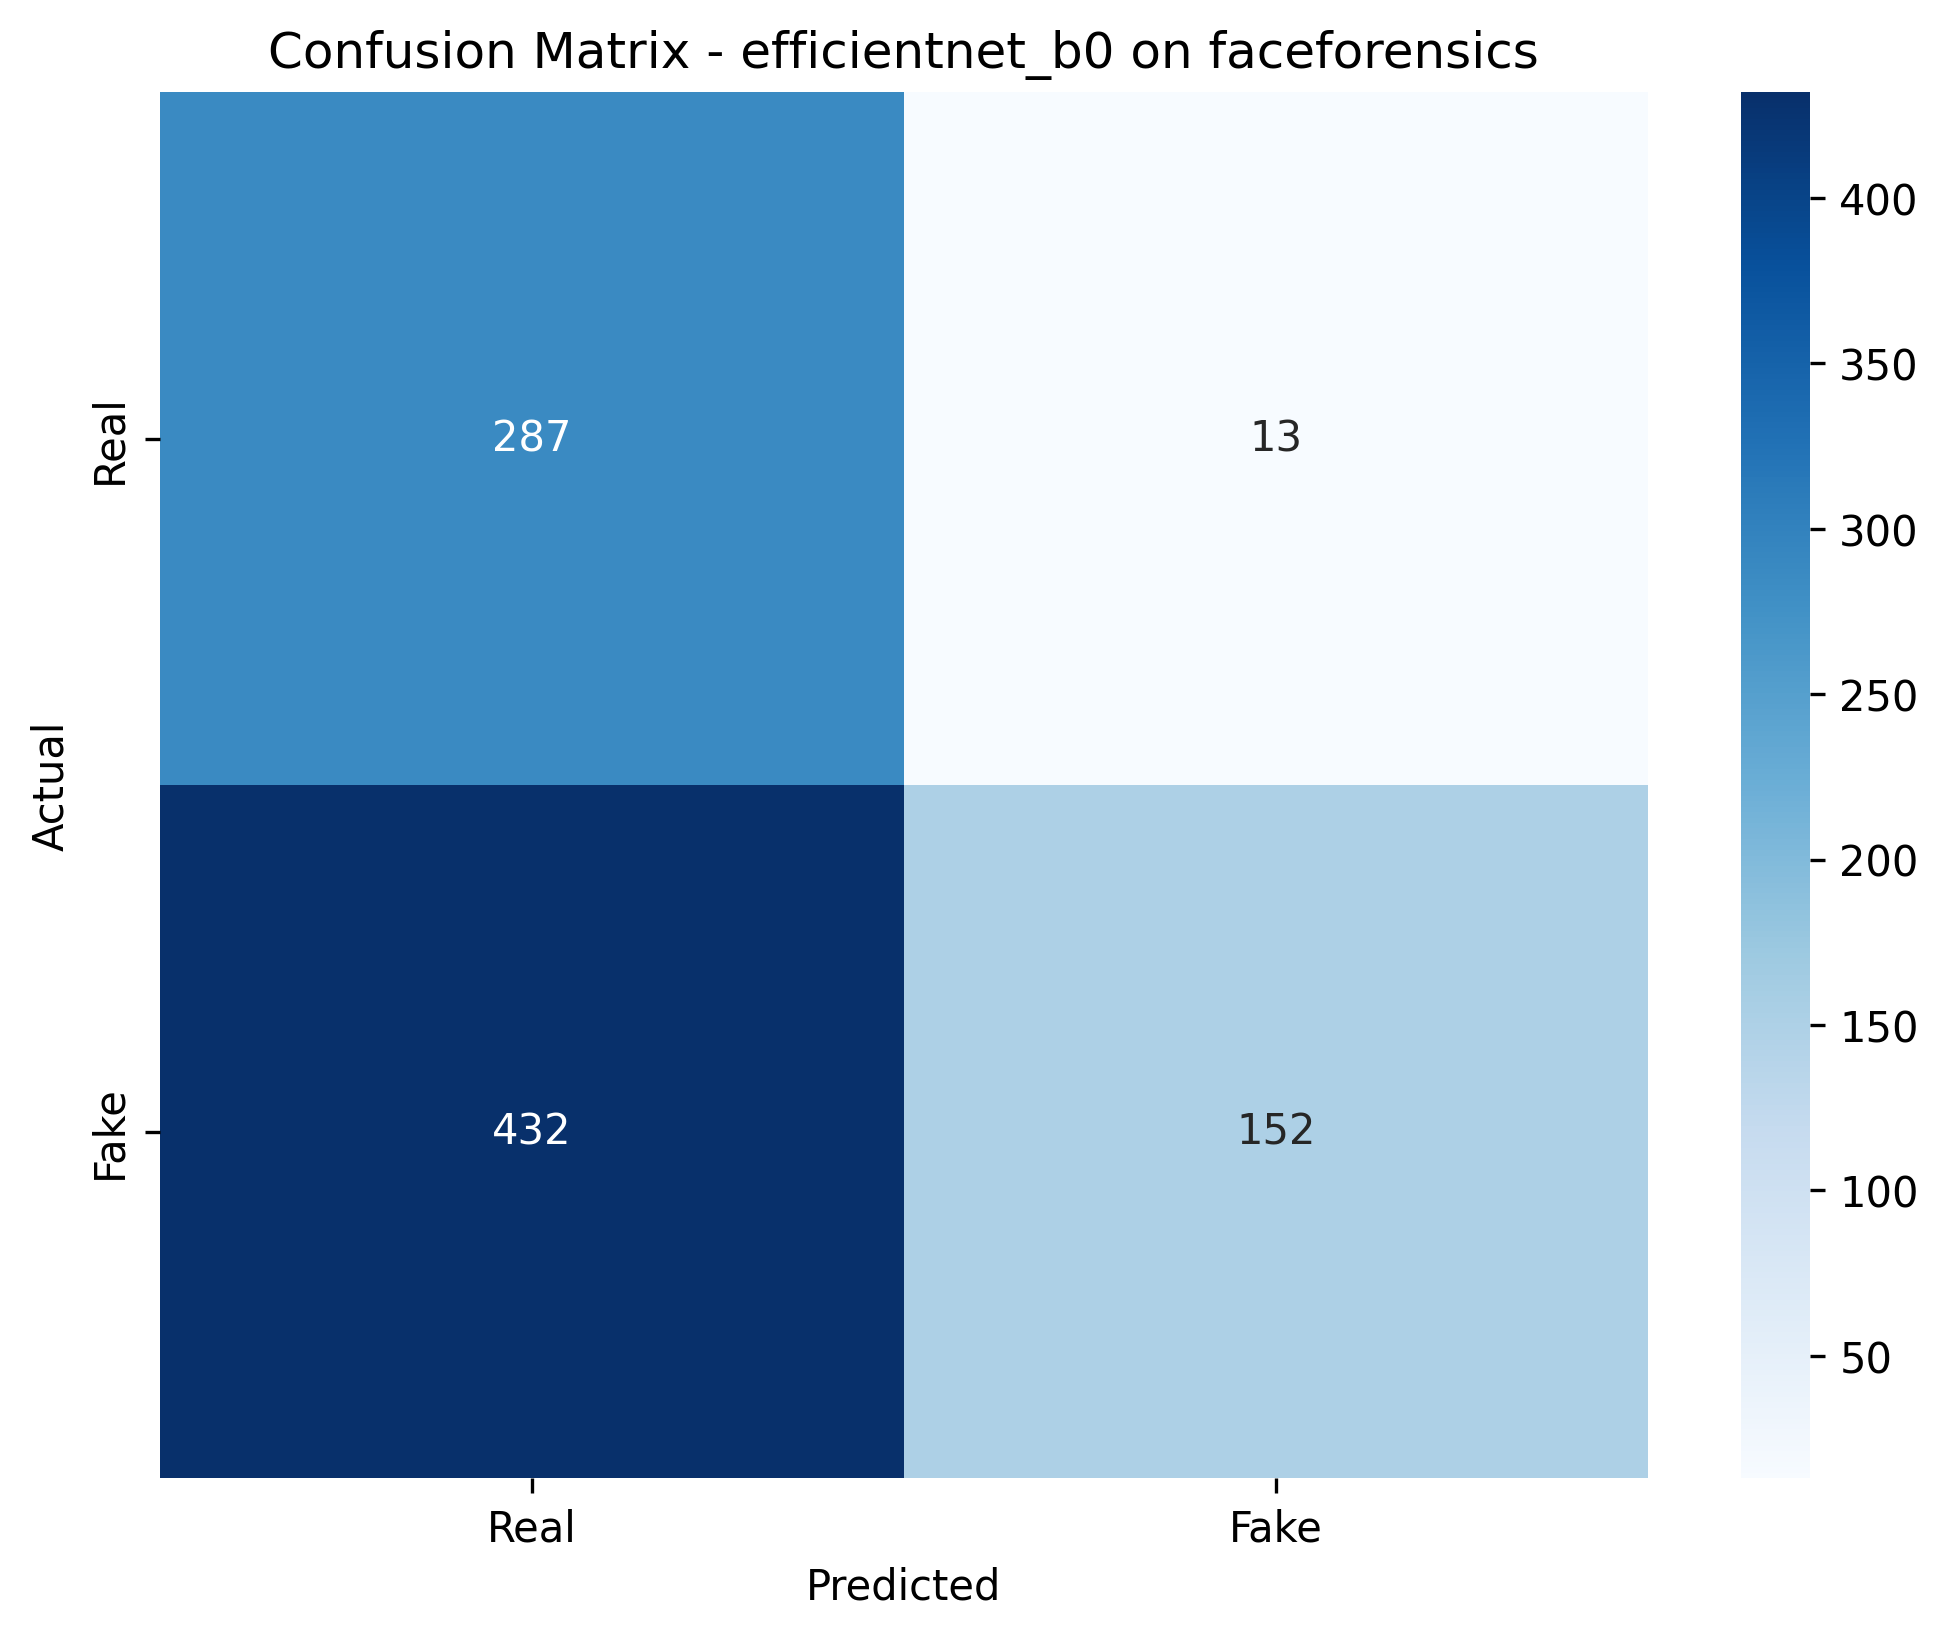
\includegraphics[width=0.20\textwidth]{figures/efficientnet_b0_faceforensics_confusion_matrix.png} &
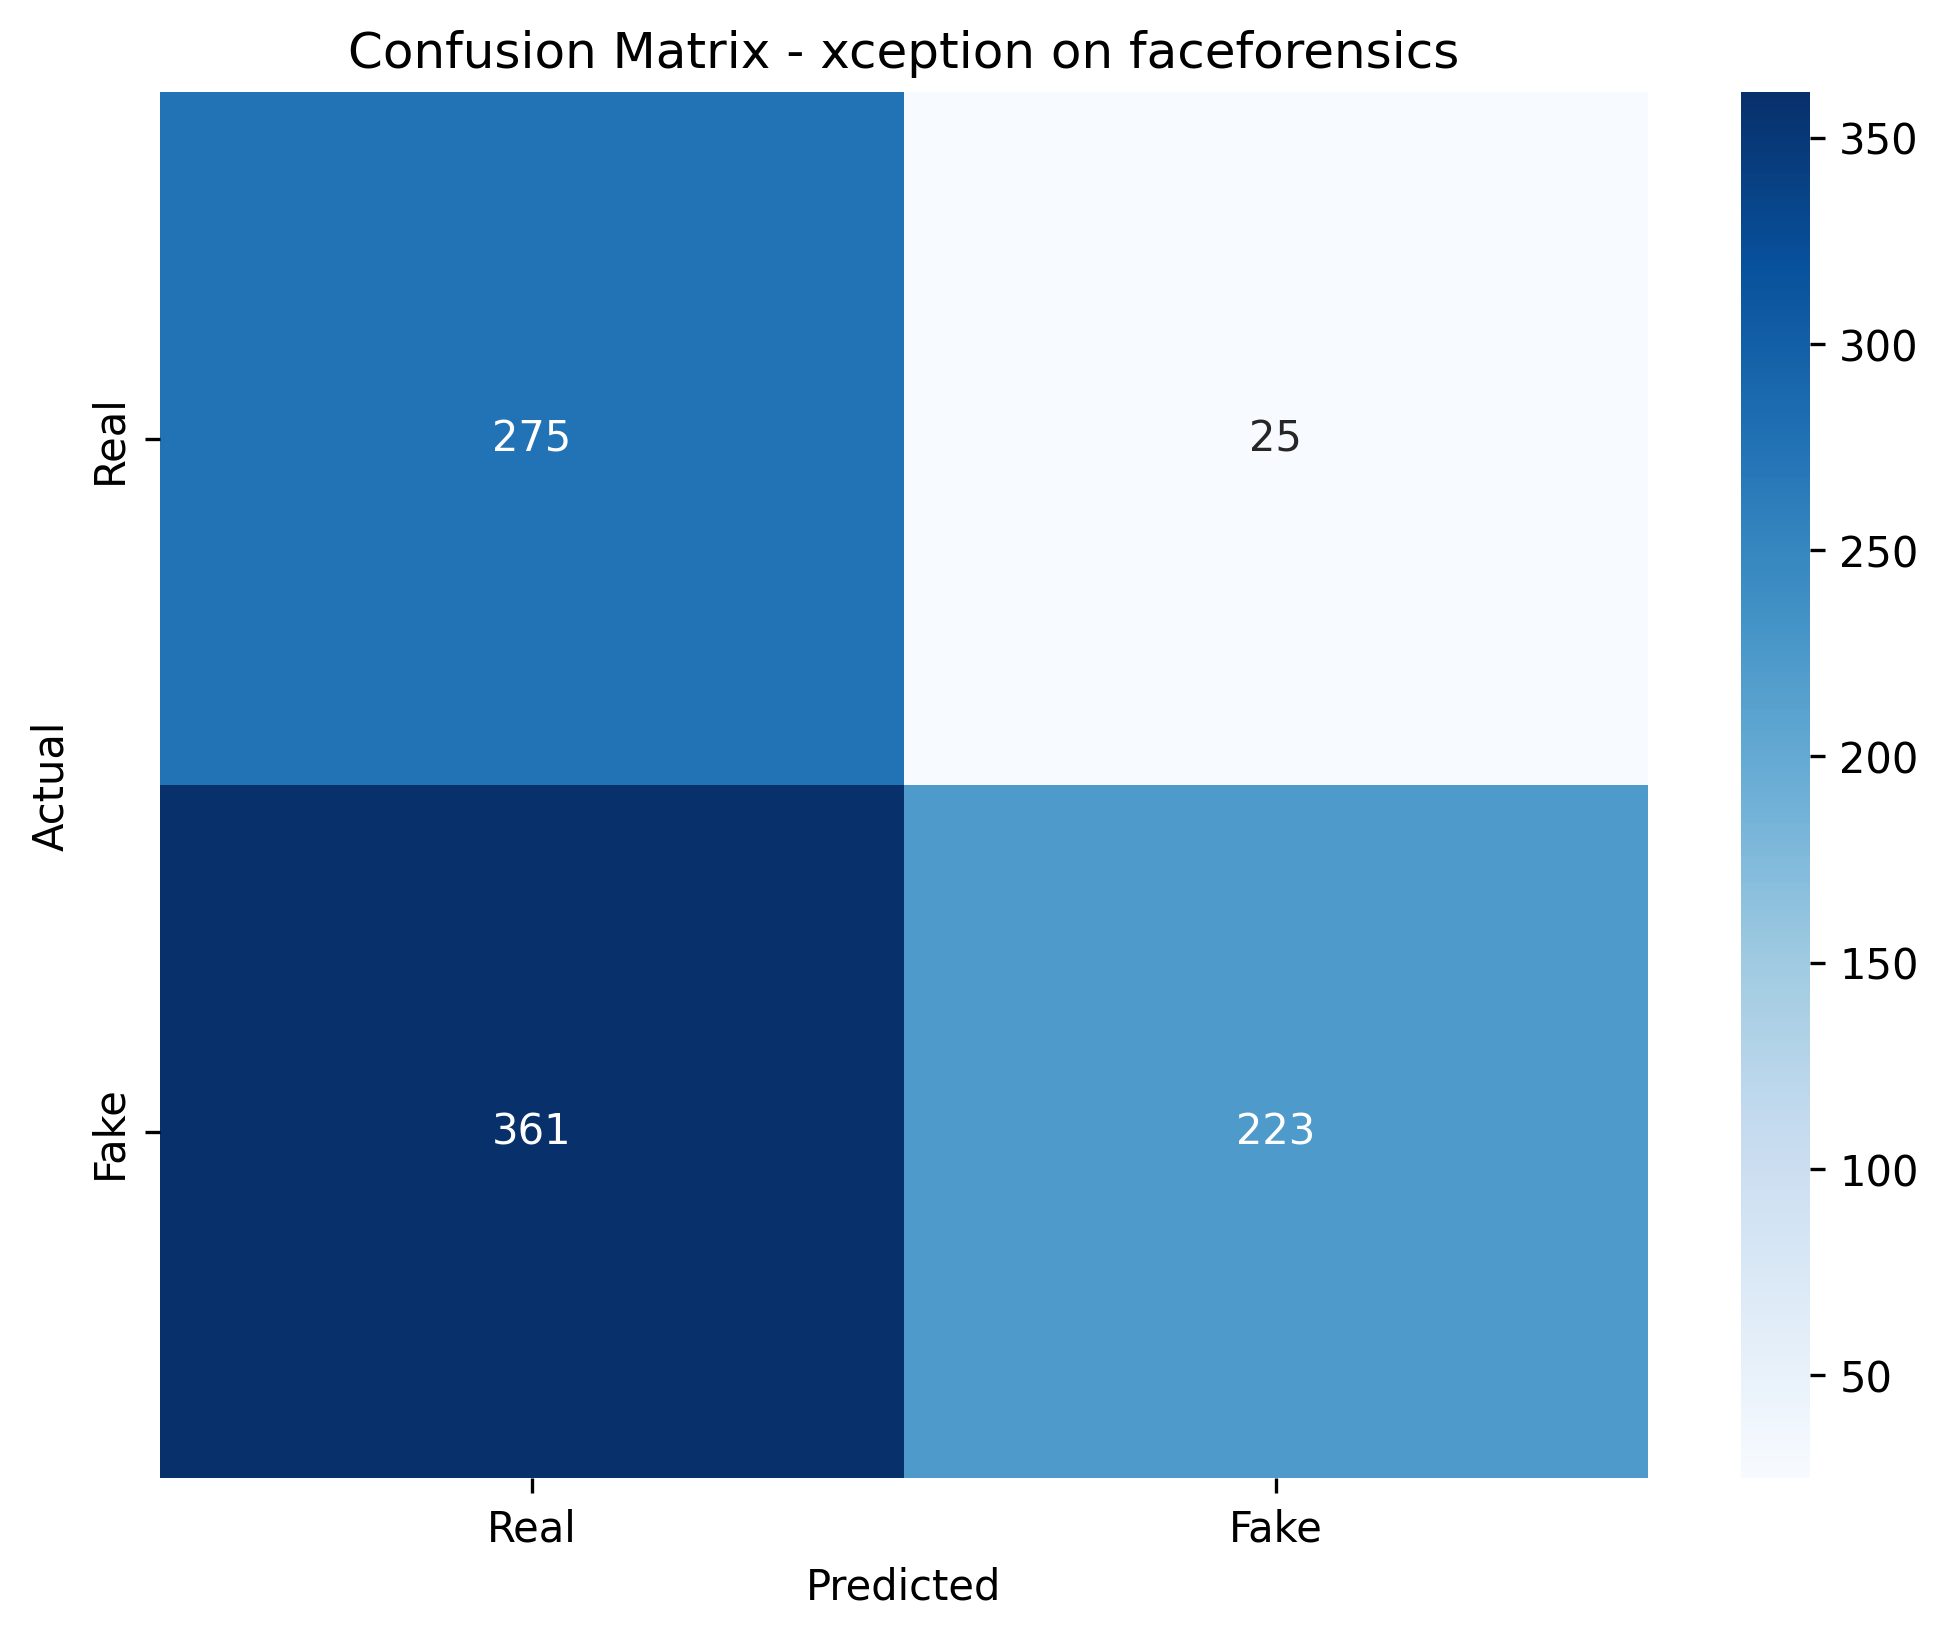
\includegraphics[width=0.20\textwidth]{figures/xception_faceforensics_confusion_matrix.png} \\
(a) EfficientNet-B0 & (b) XceptionNet \\
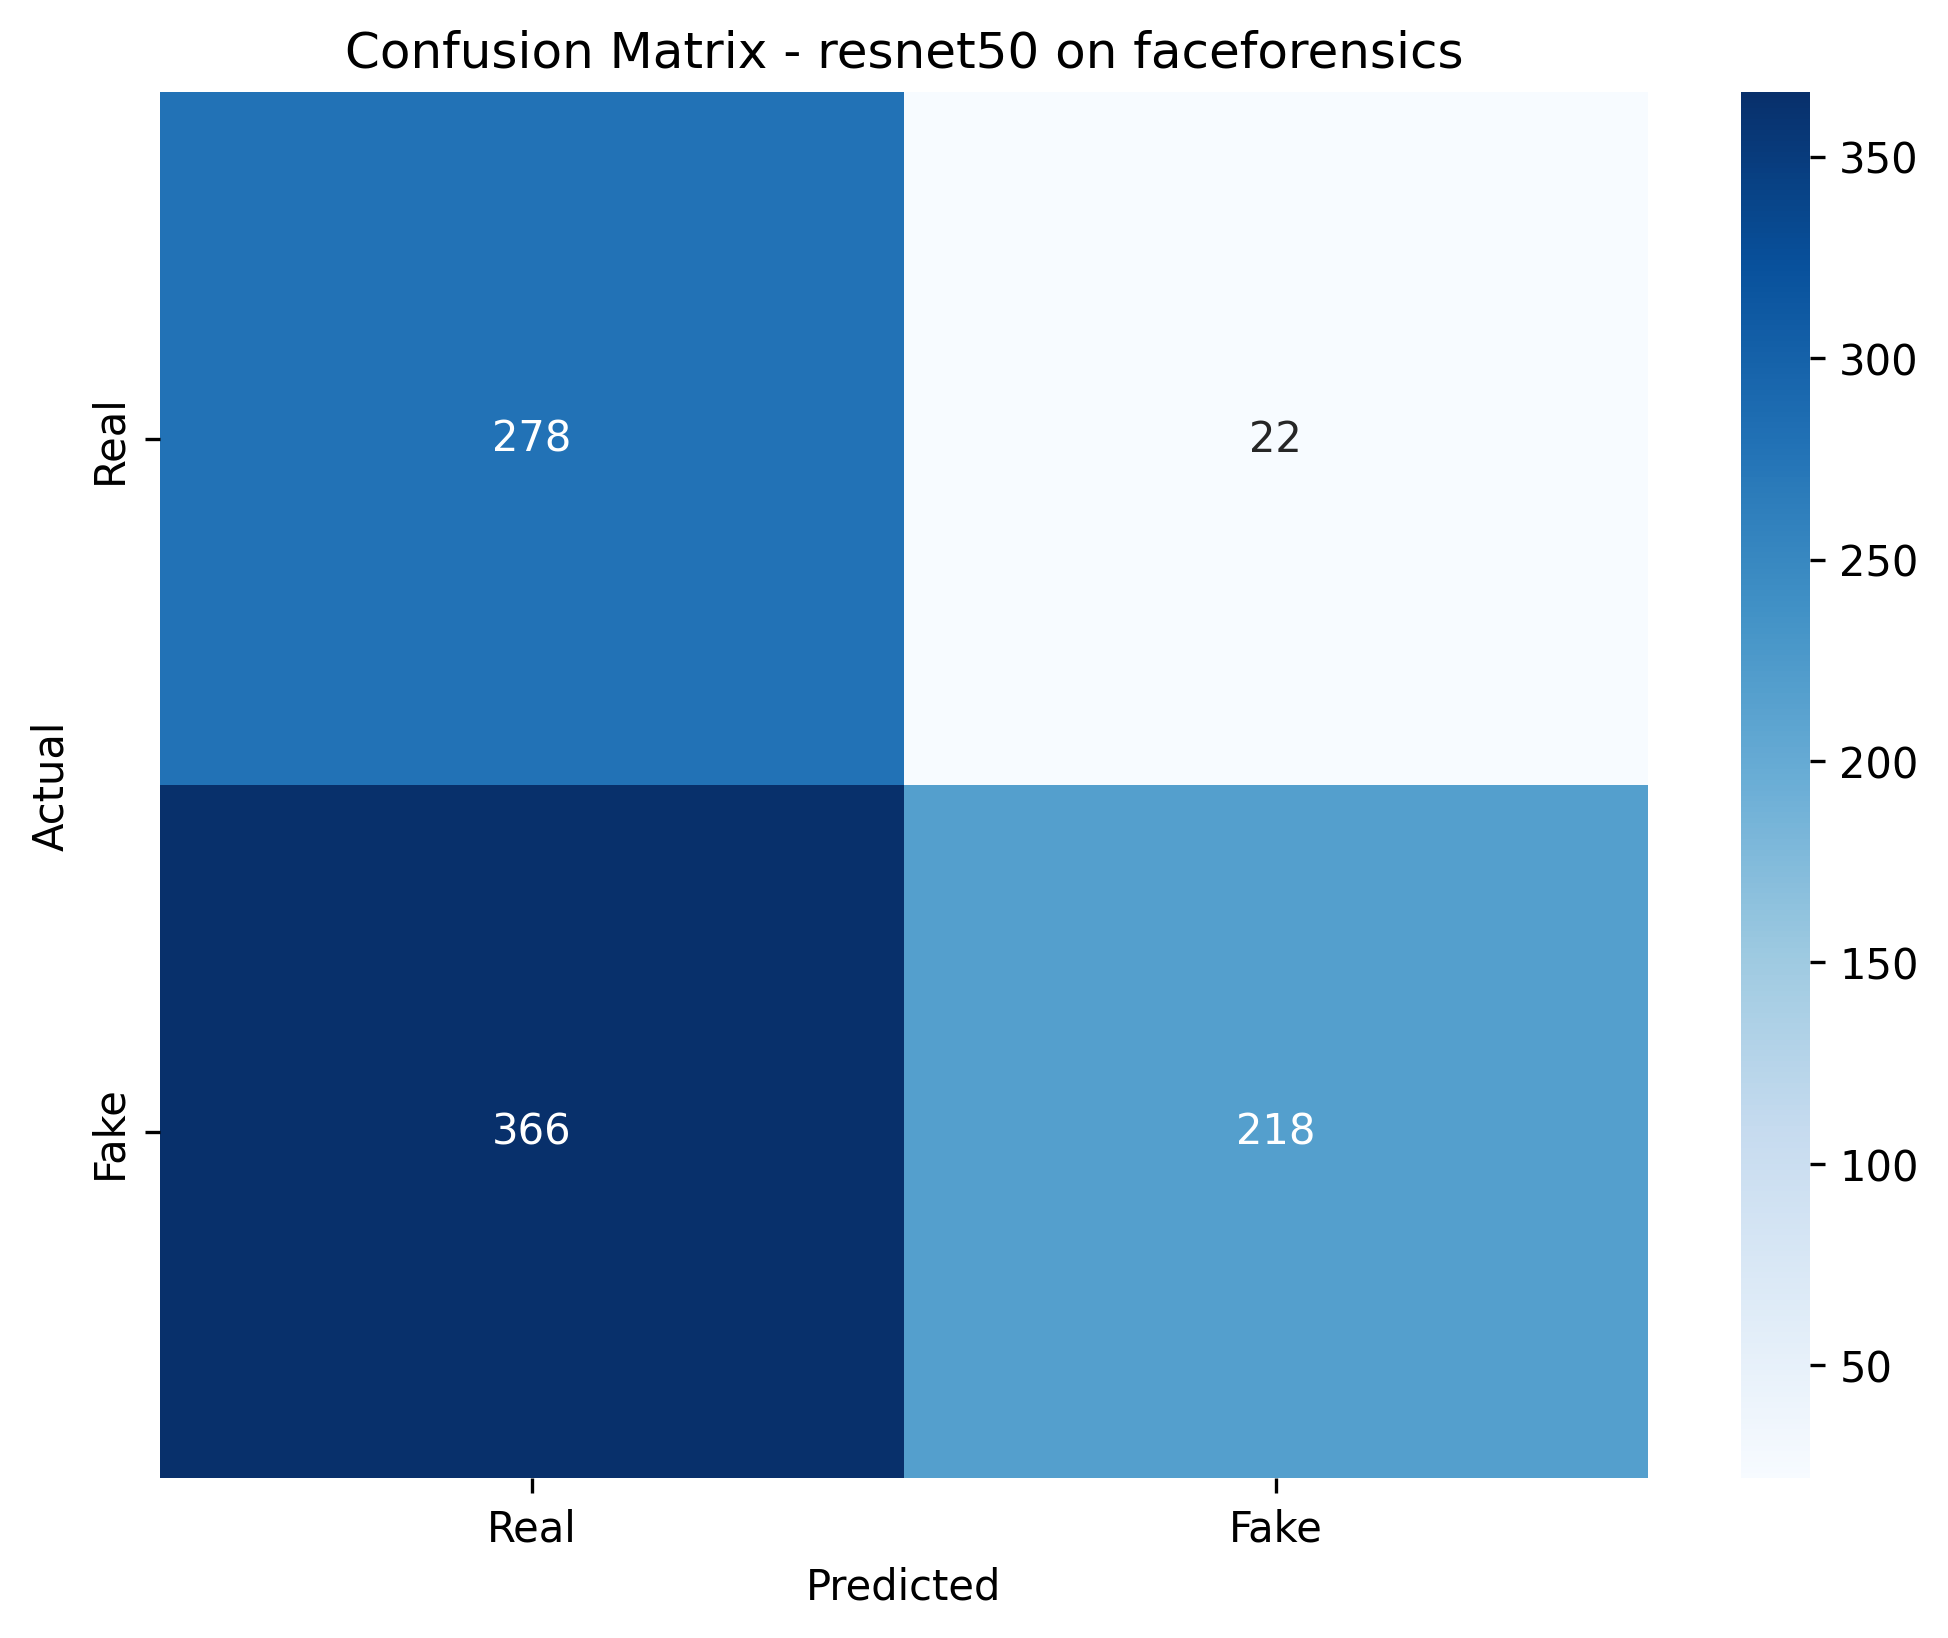
\includegraphics[width=0.20\textwidth]{figures/resnet50_faceforensics_confusion_matrix.png} &
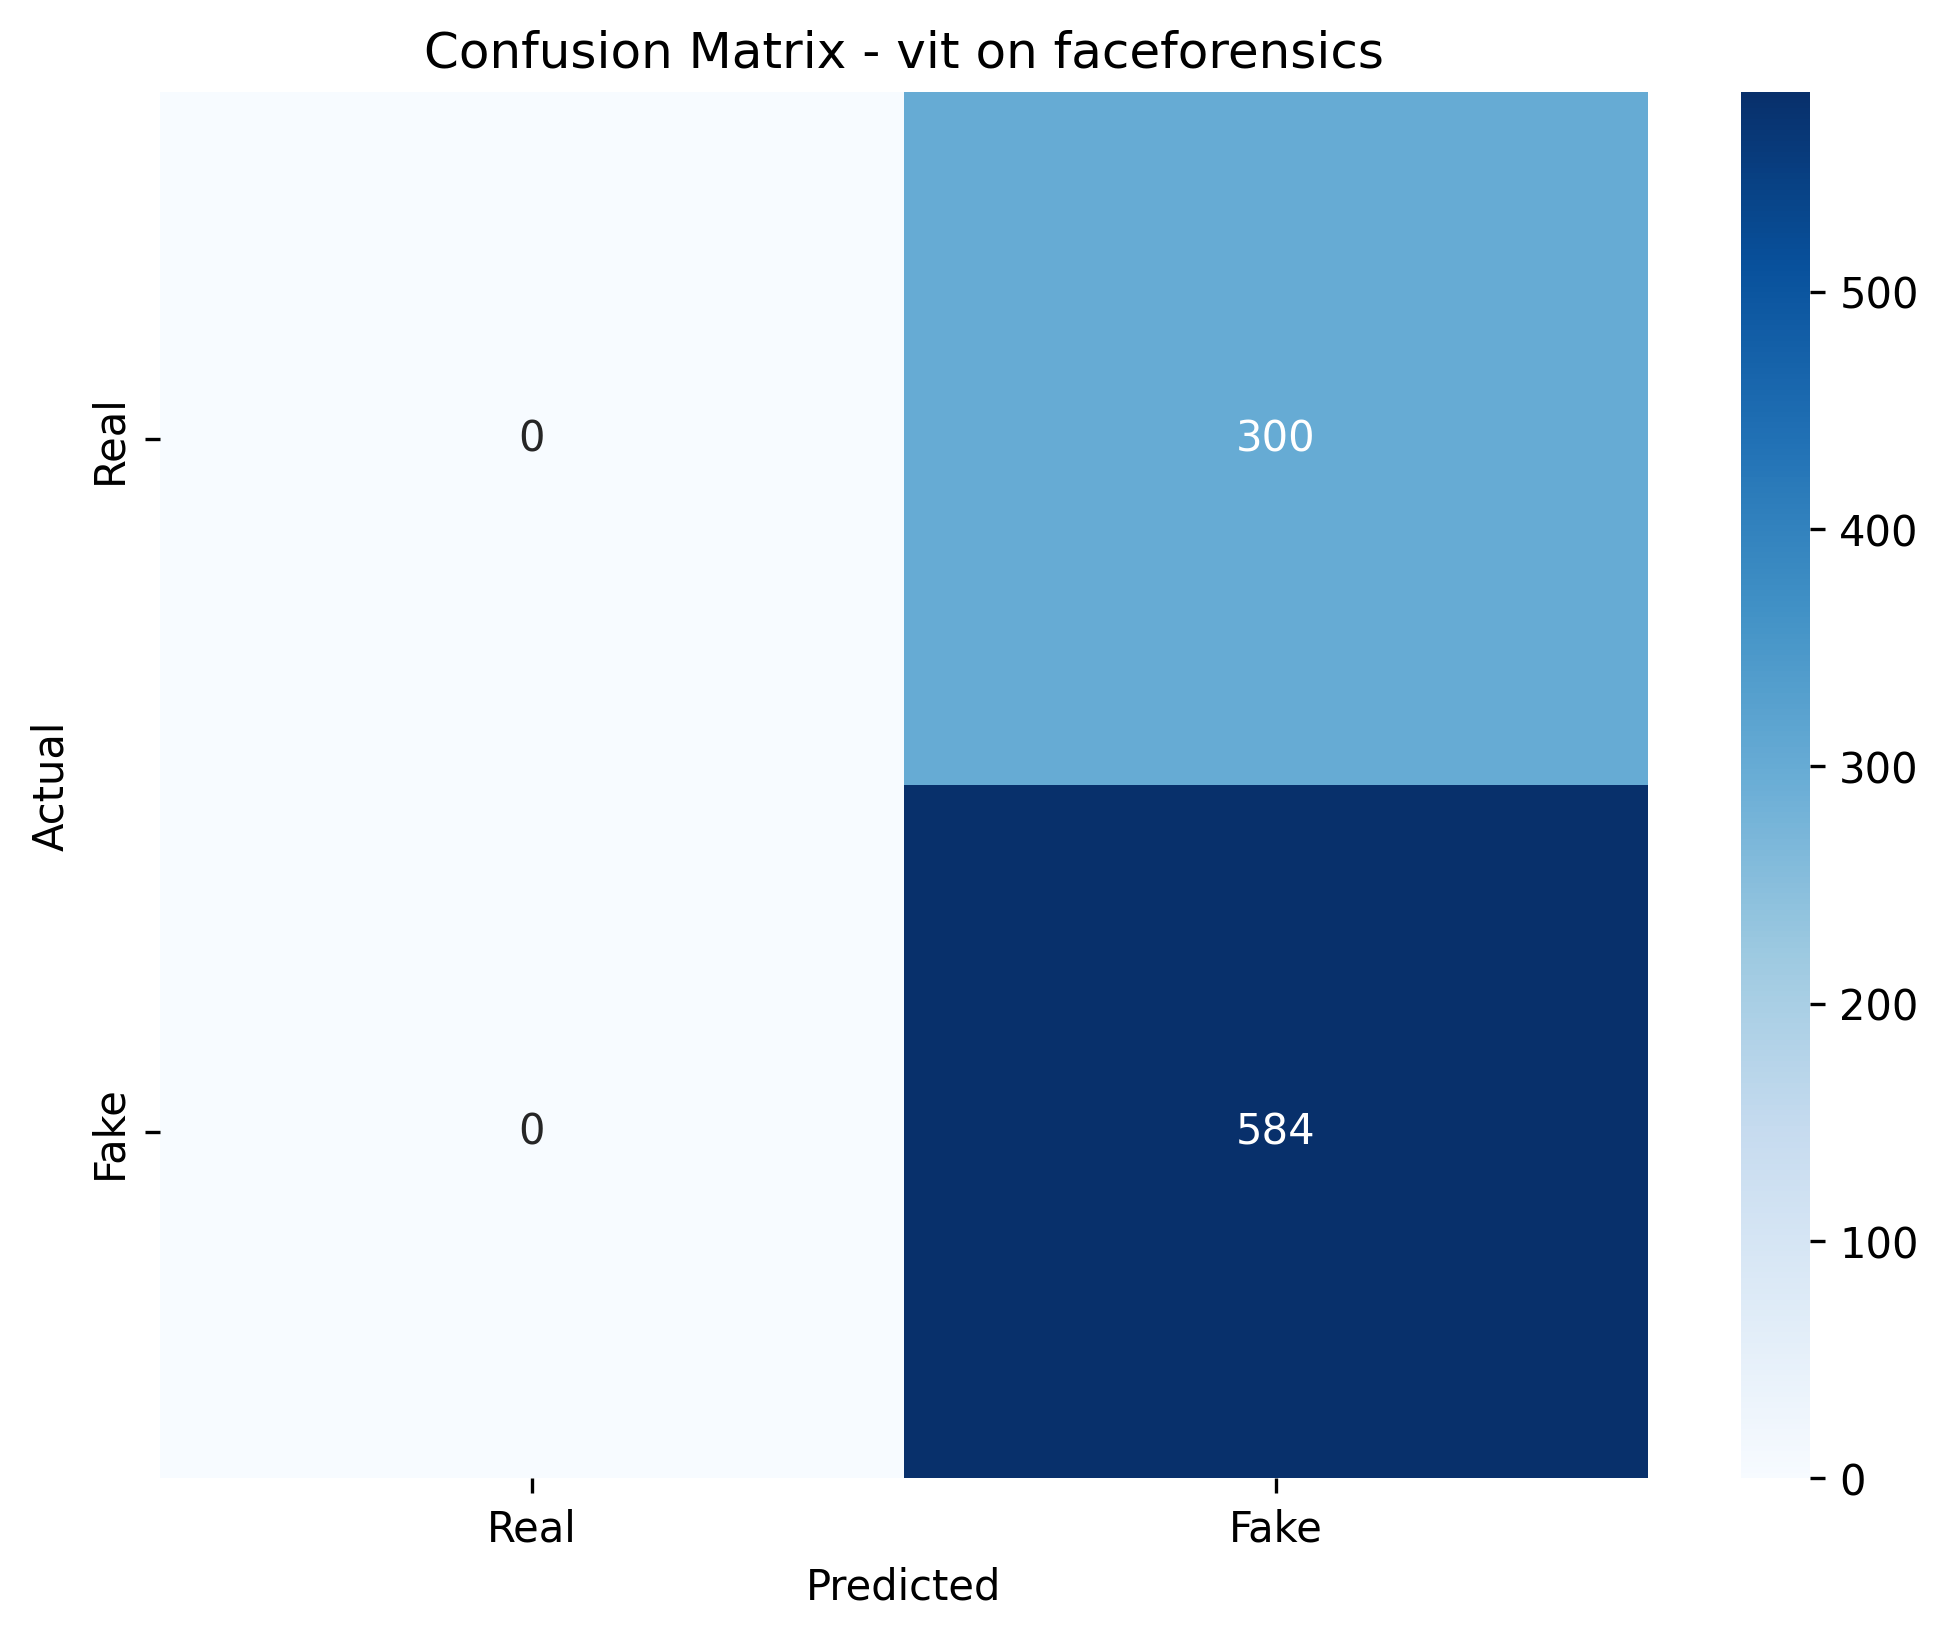
\includegraphics[width=0.20\textwidth]{figures/vit_faceforensics_confusion_matrix.png} \\
(c) ResNet50 & (d) Vision Transformer
\end{tabular}
\caption{Confusion matrices for cross-dataset evaluation (Celeb-DF trained models tested on FaceForensics++).}
\label{fig:confusion_ff}
\end{figure*}

\begin{figure*}[!htbp]
\centering
\begin{tabular}{cc}
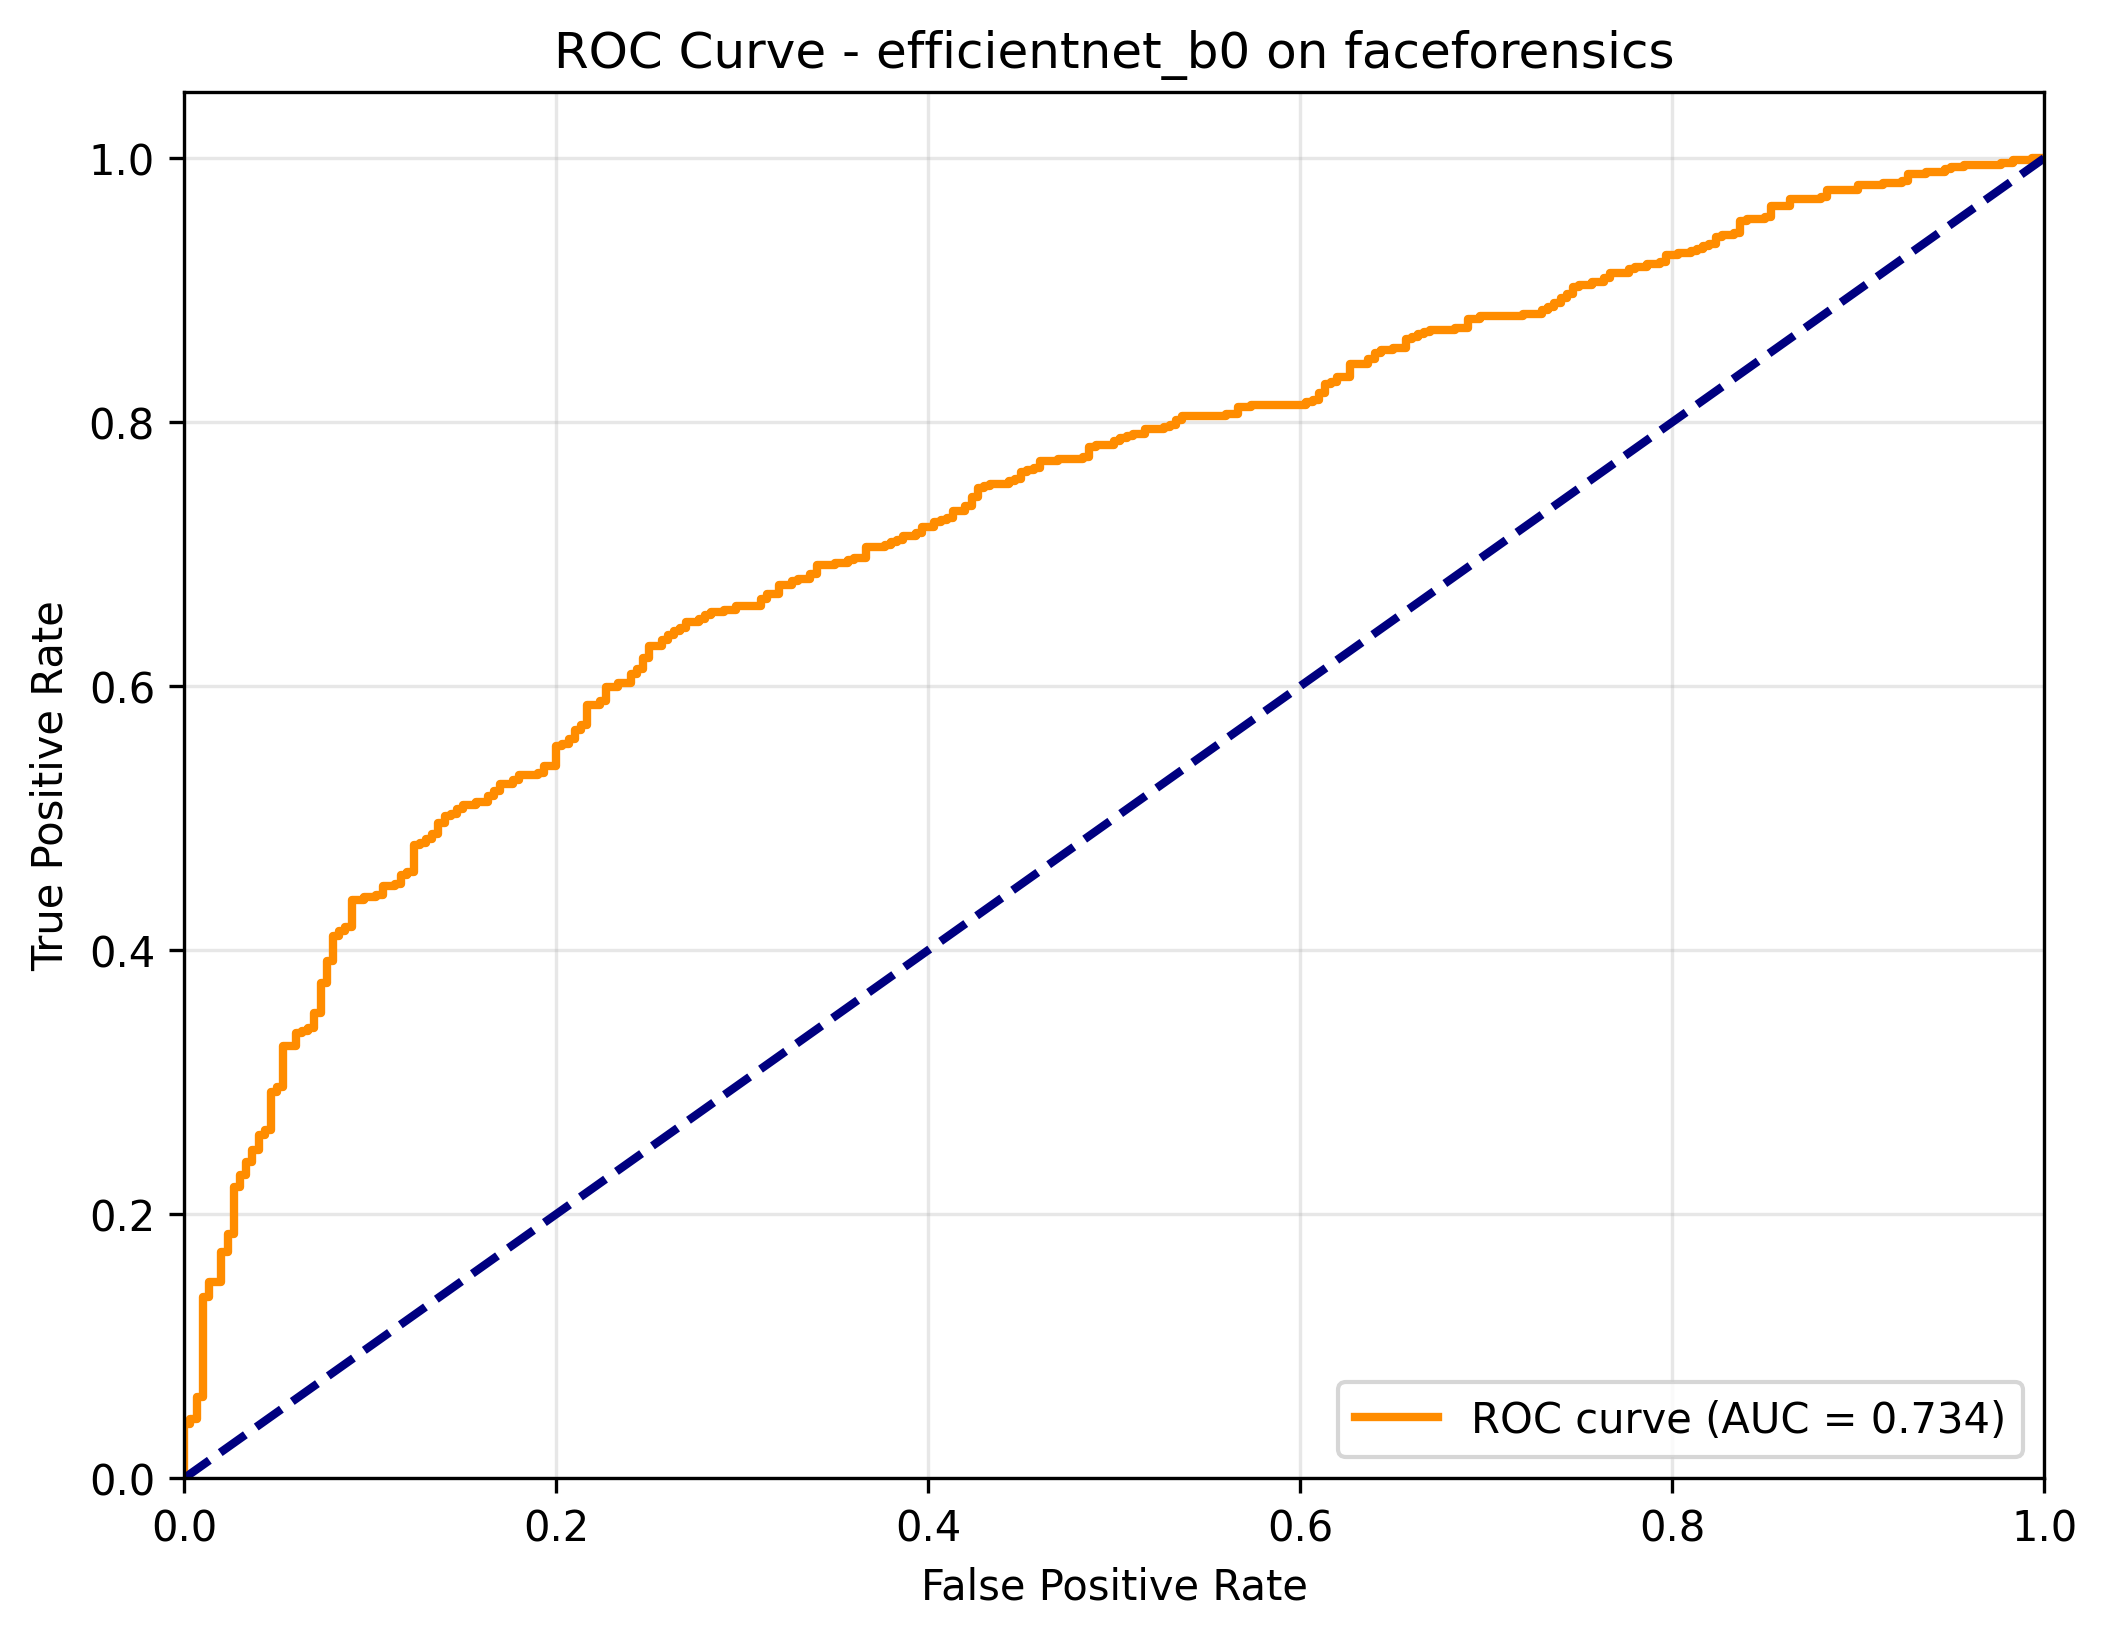
\includegraphics[width=0.20\textwidth]{figures/efficientnet_b0_faceforensics_roc_curve.png} &
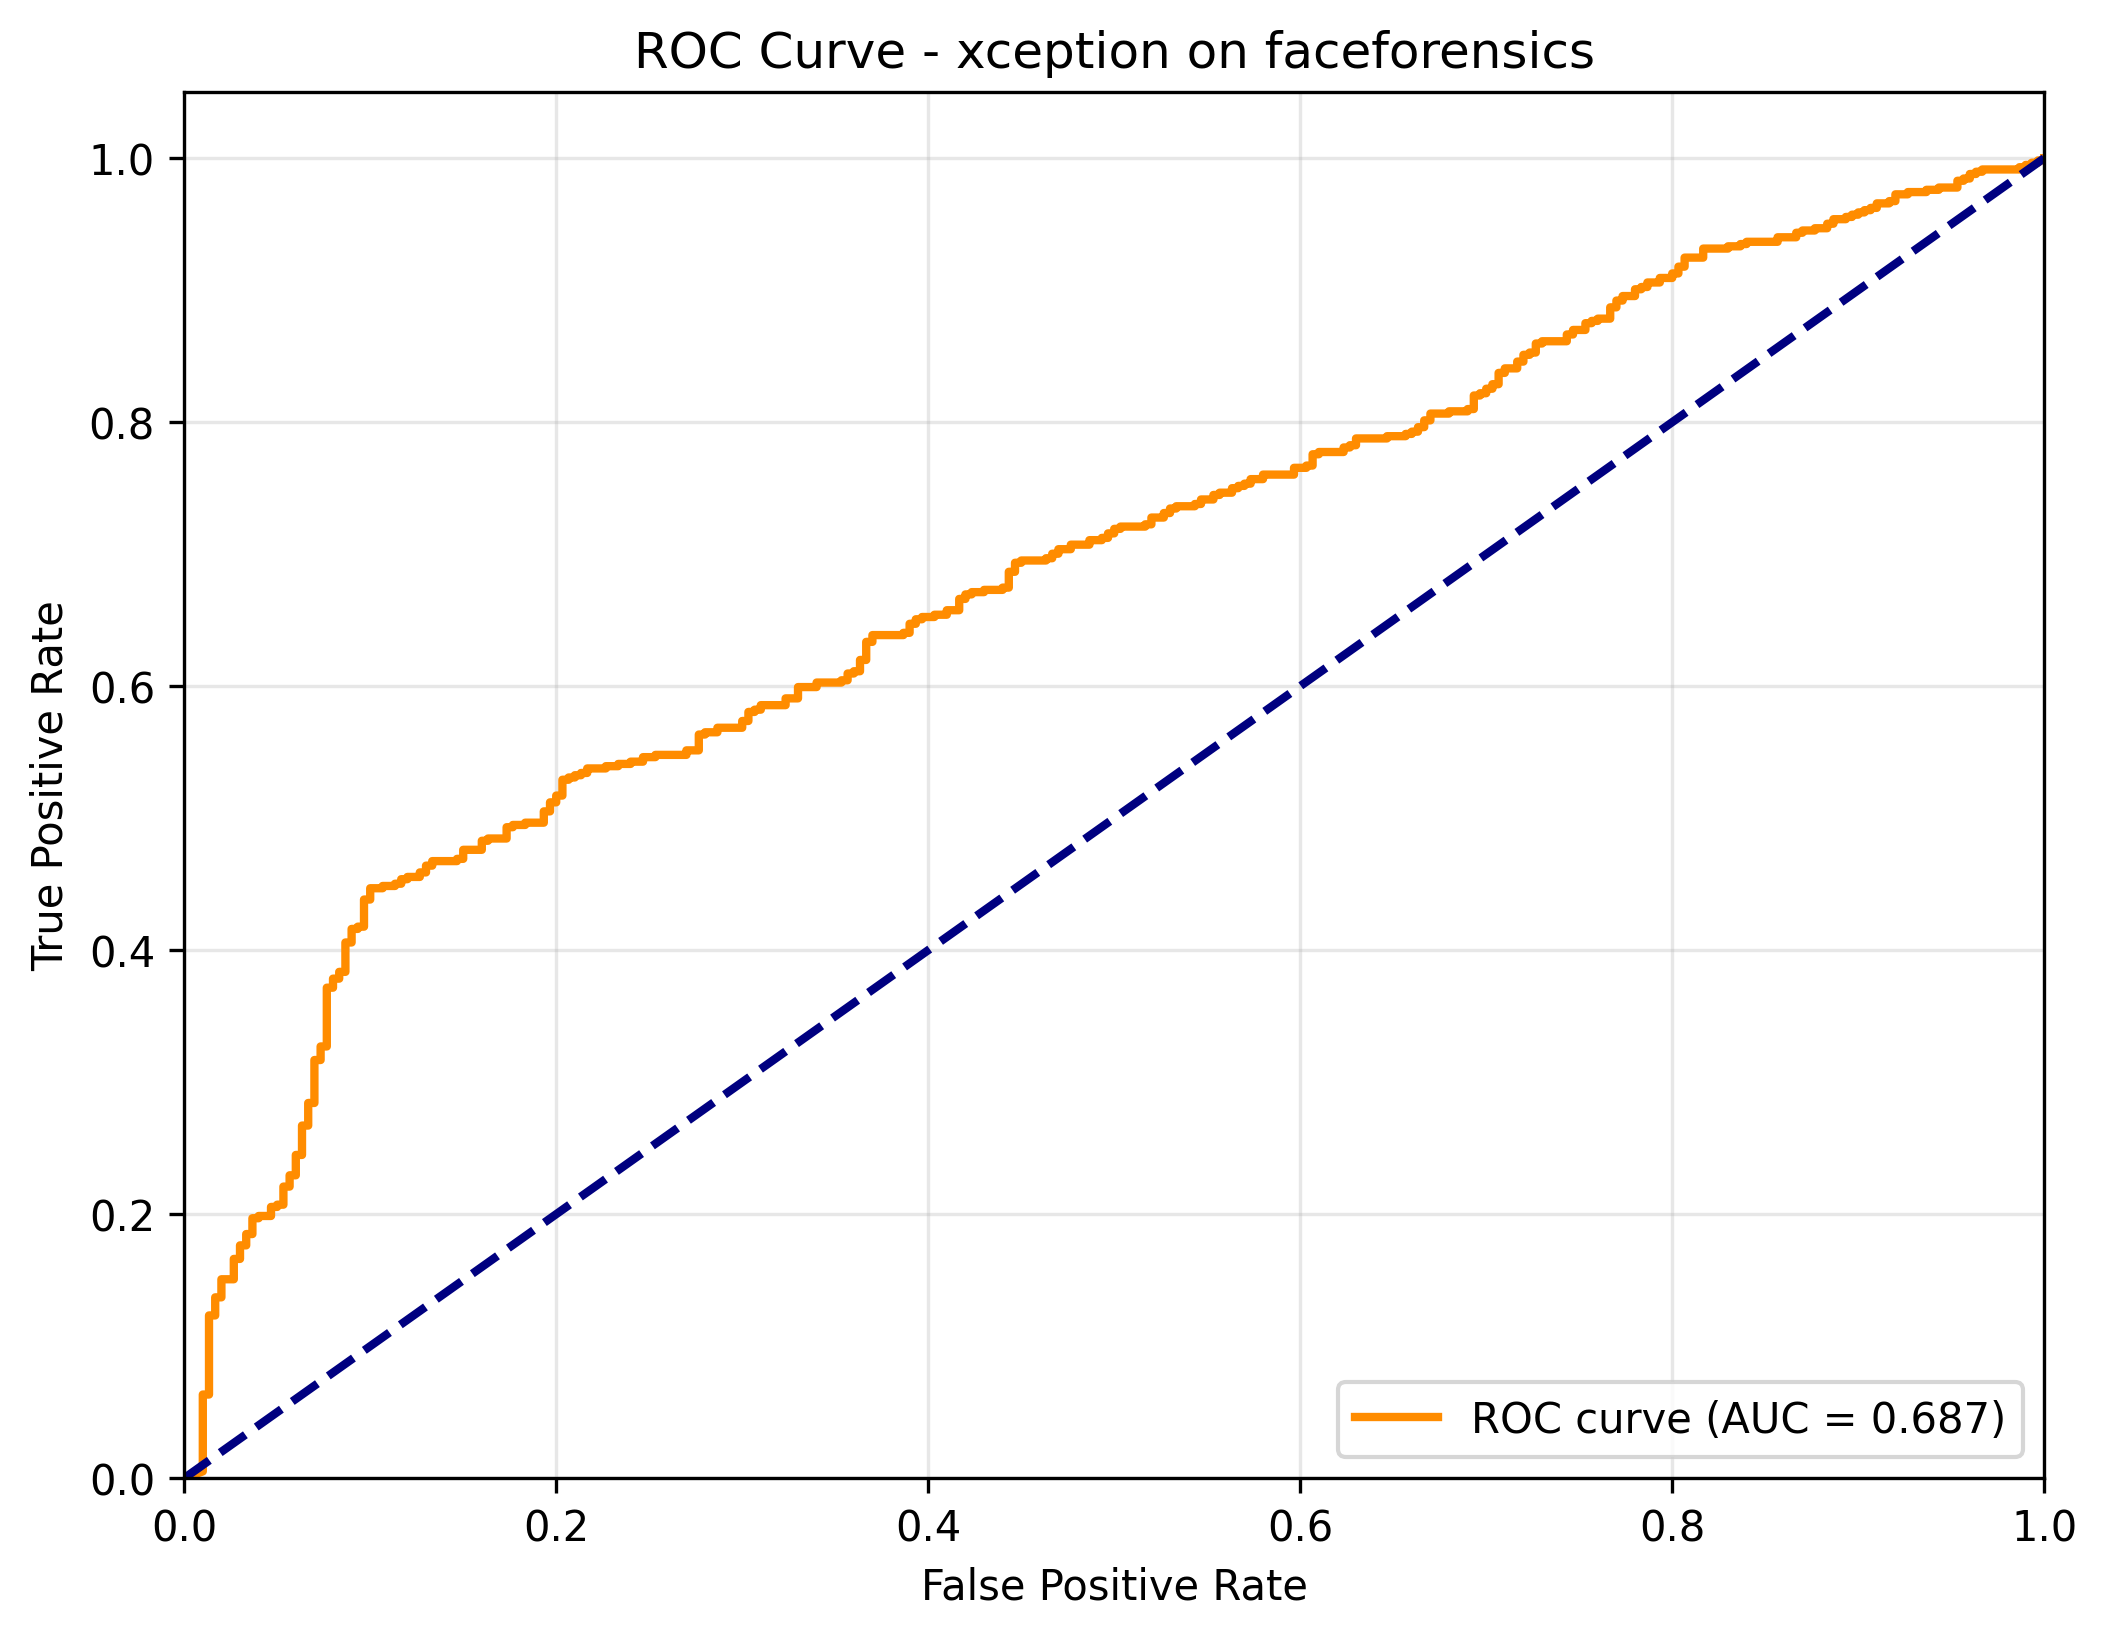
\includegraphics[width=0.20\textwidth]{figures/xception_faceforensics_roc_curve.png} \\
(a) EfficientNet-B0 & (b) XceptionNet \\
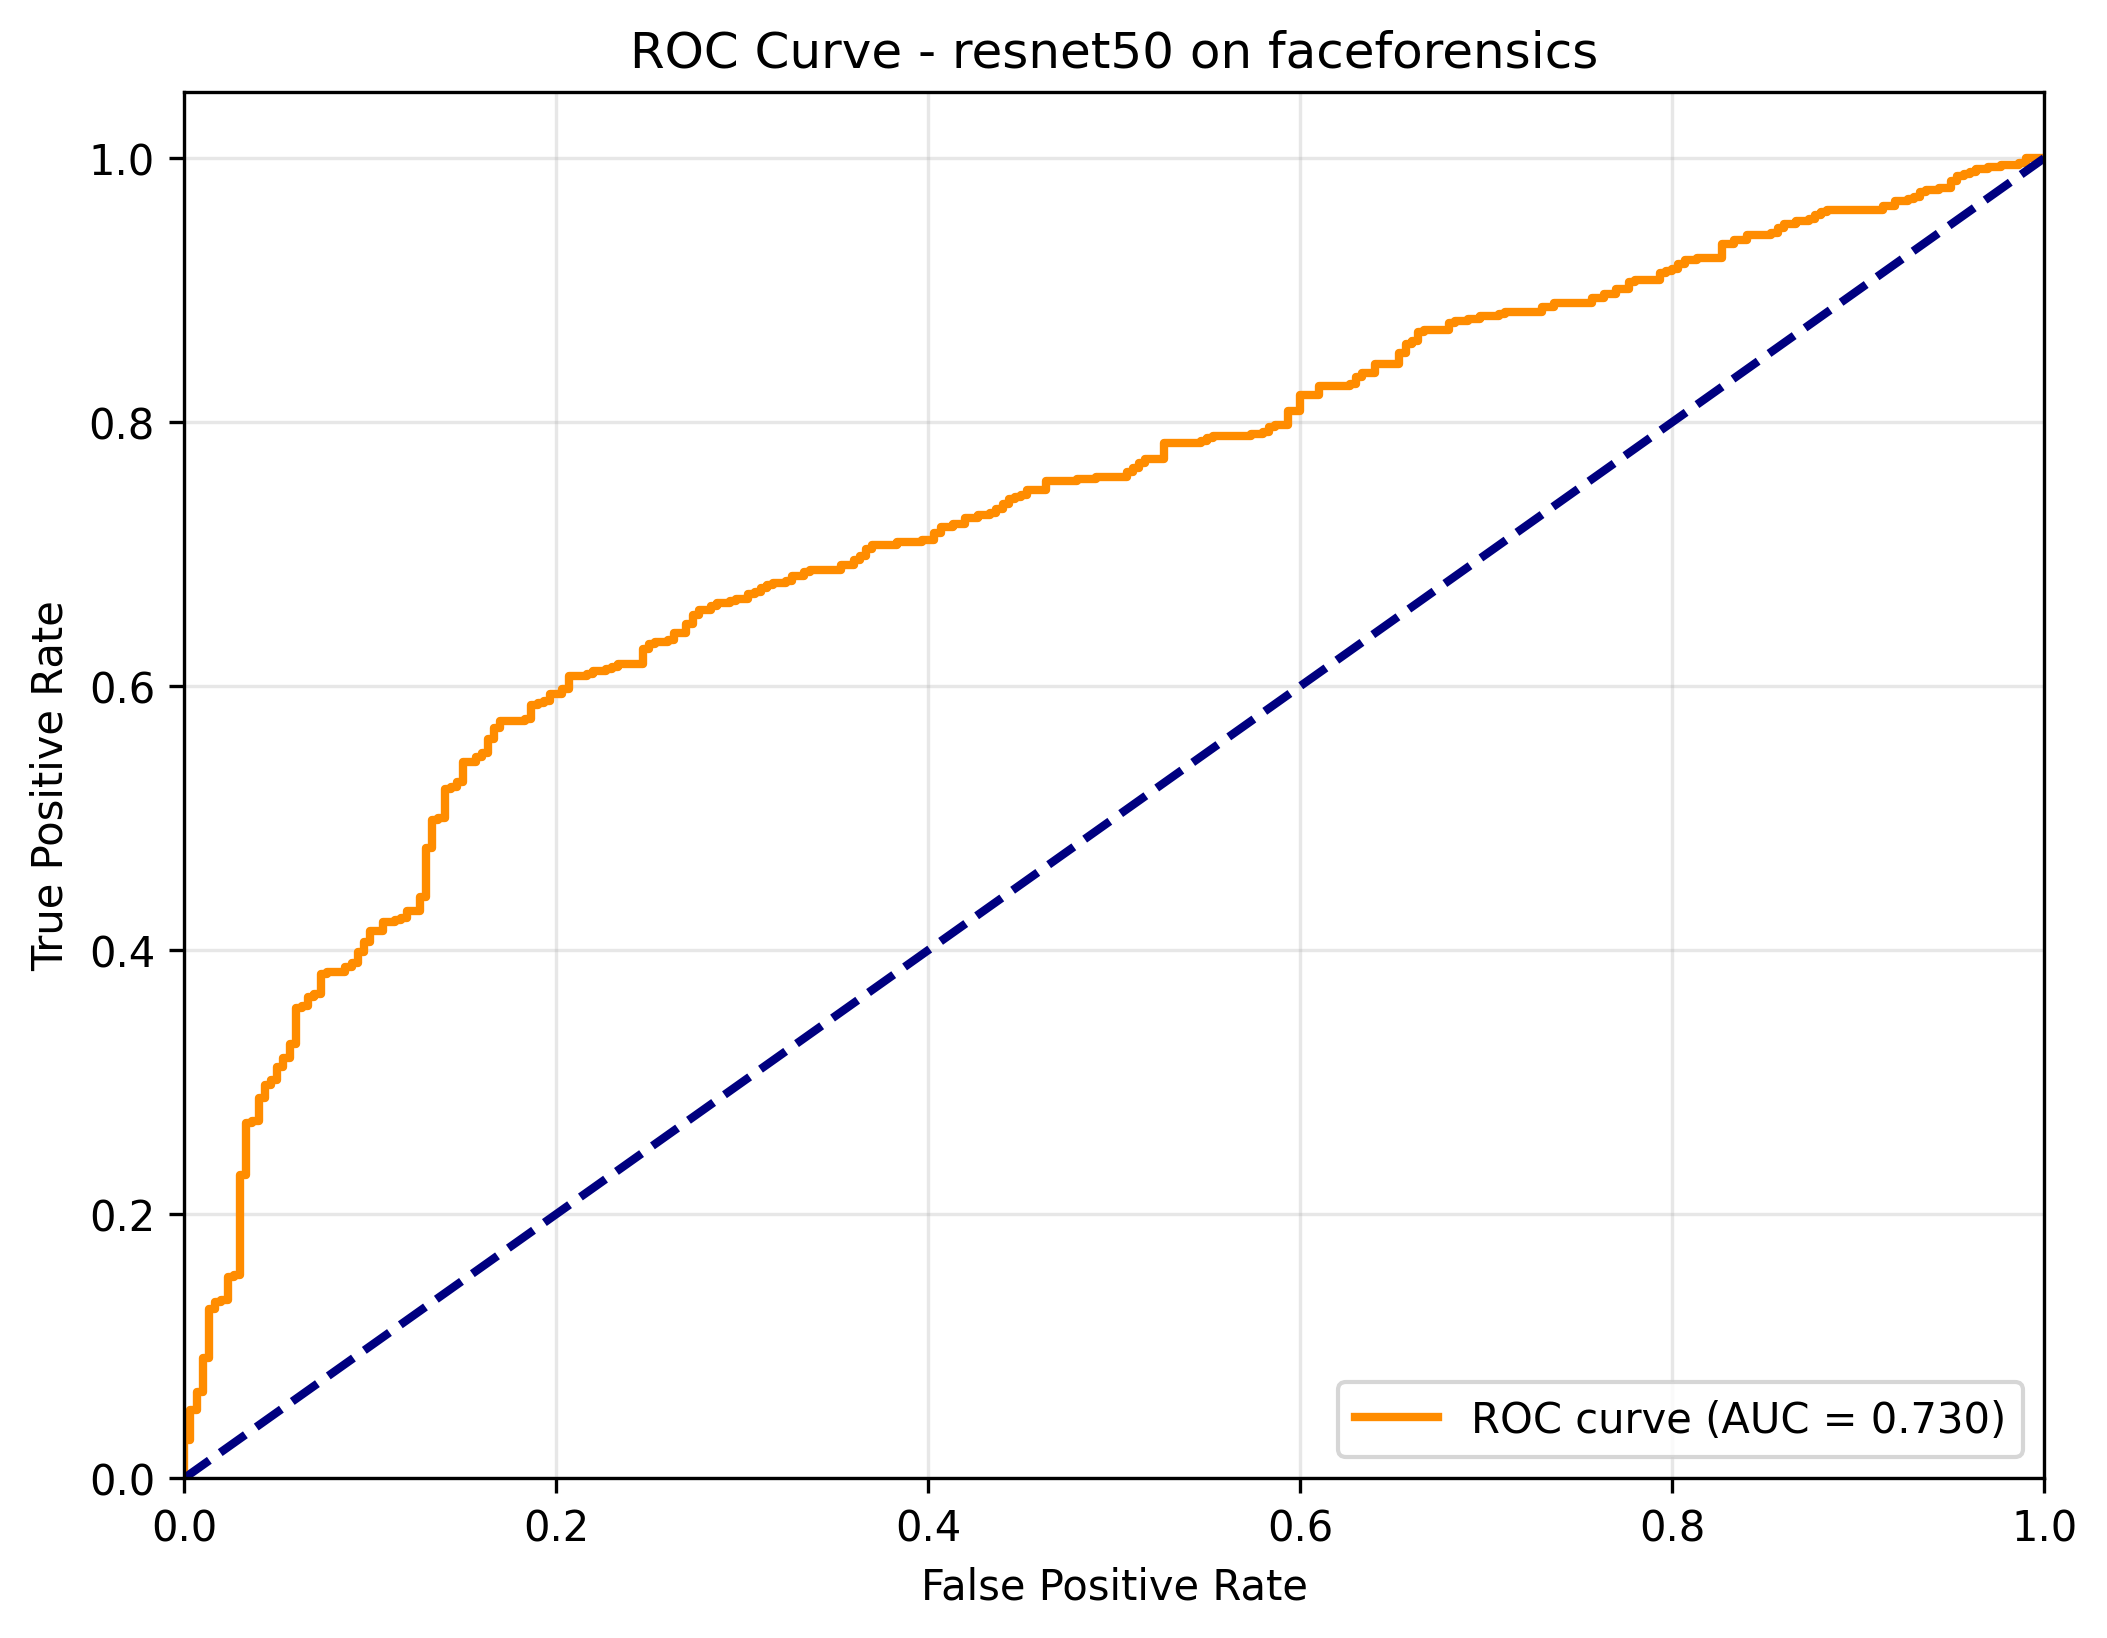
\includegraphics[width=0.20\textwidth]{figures/resnet50_faceforensics_roc_curve.png} &
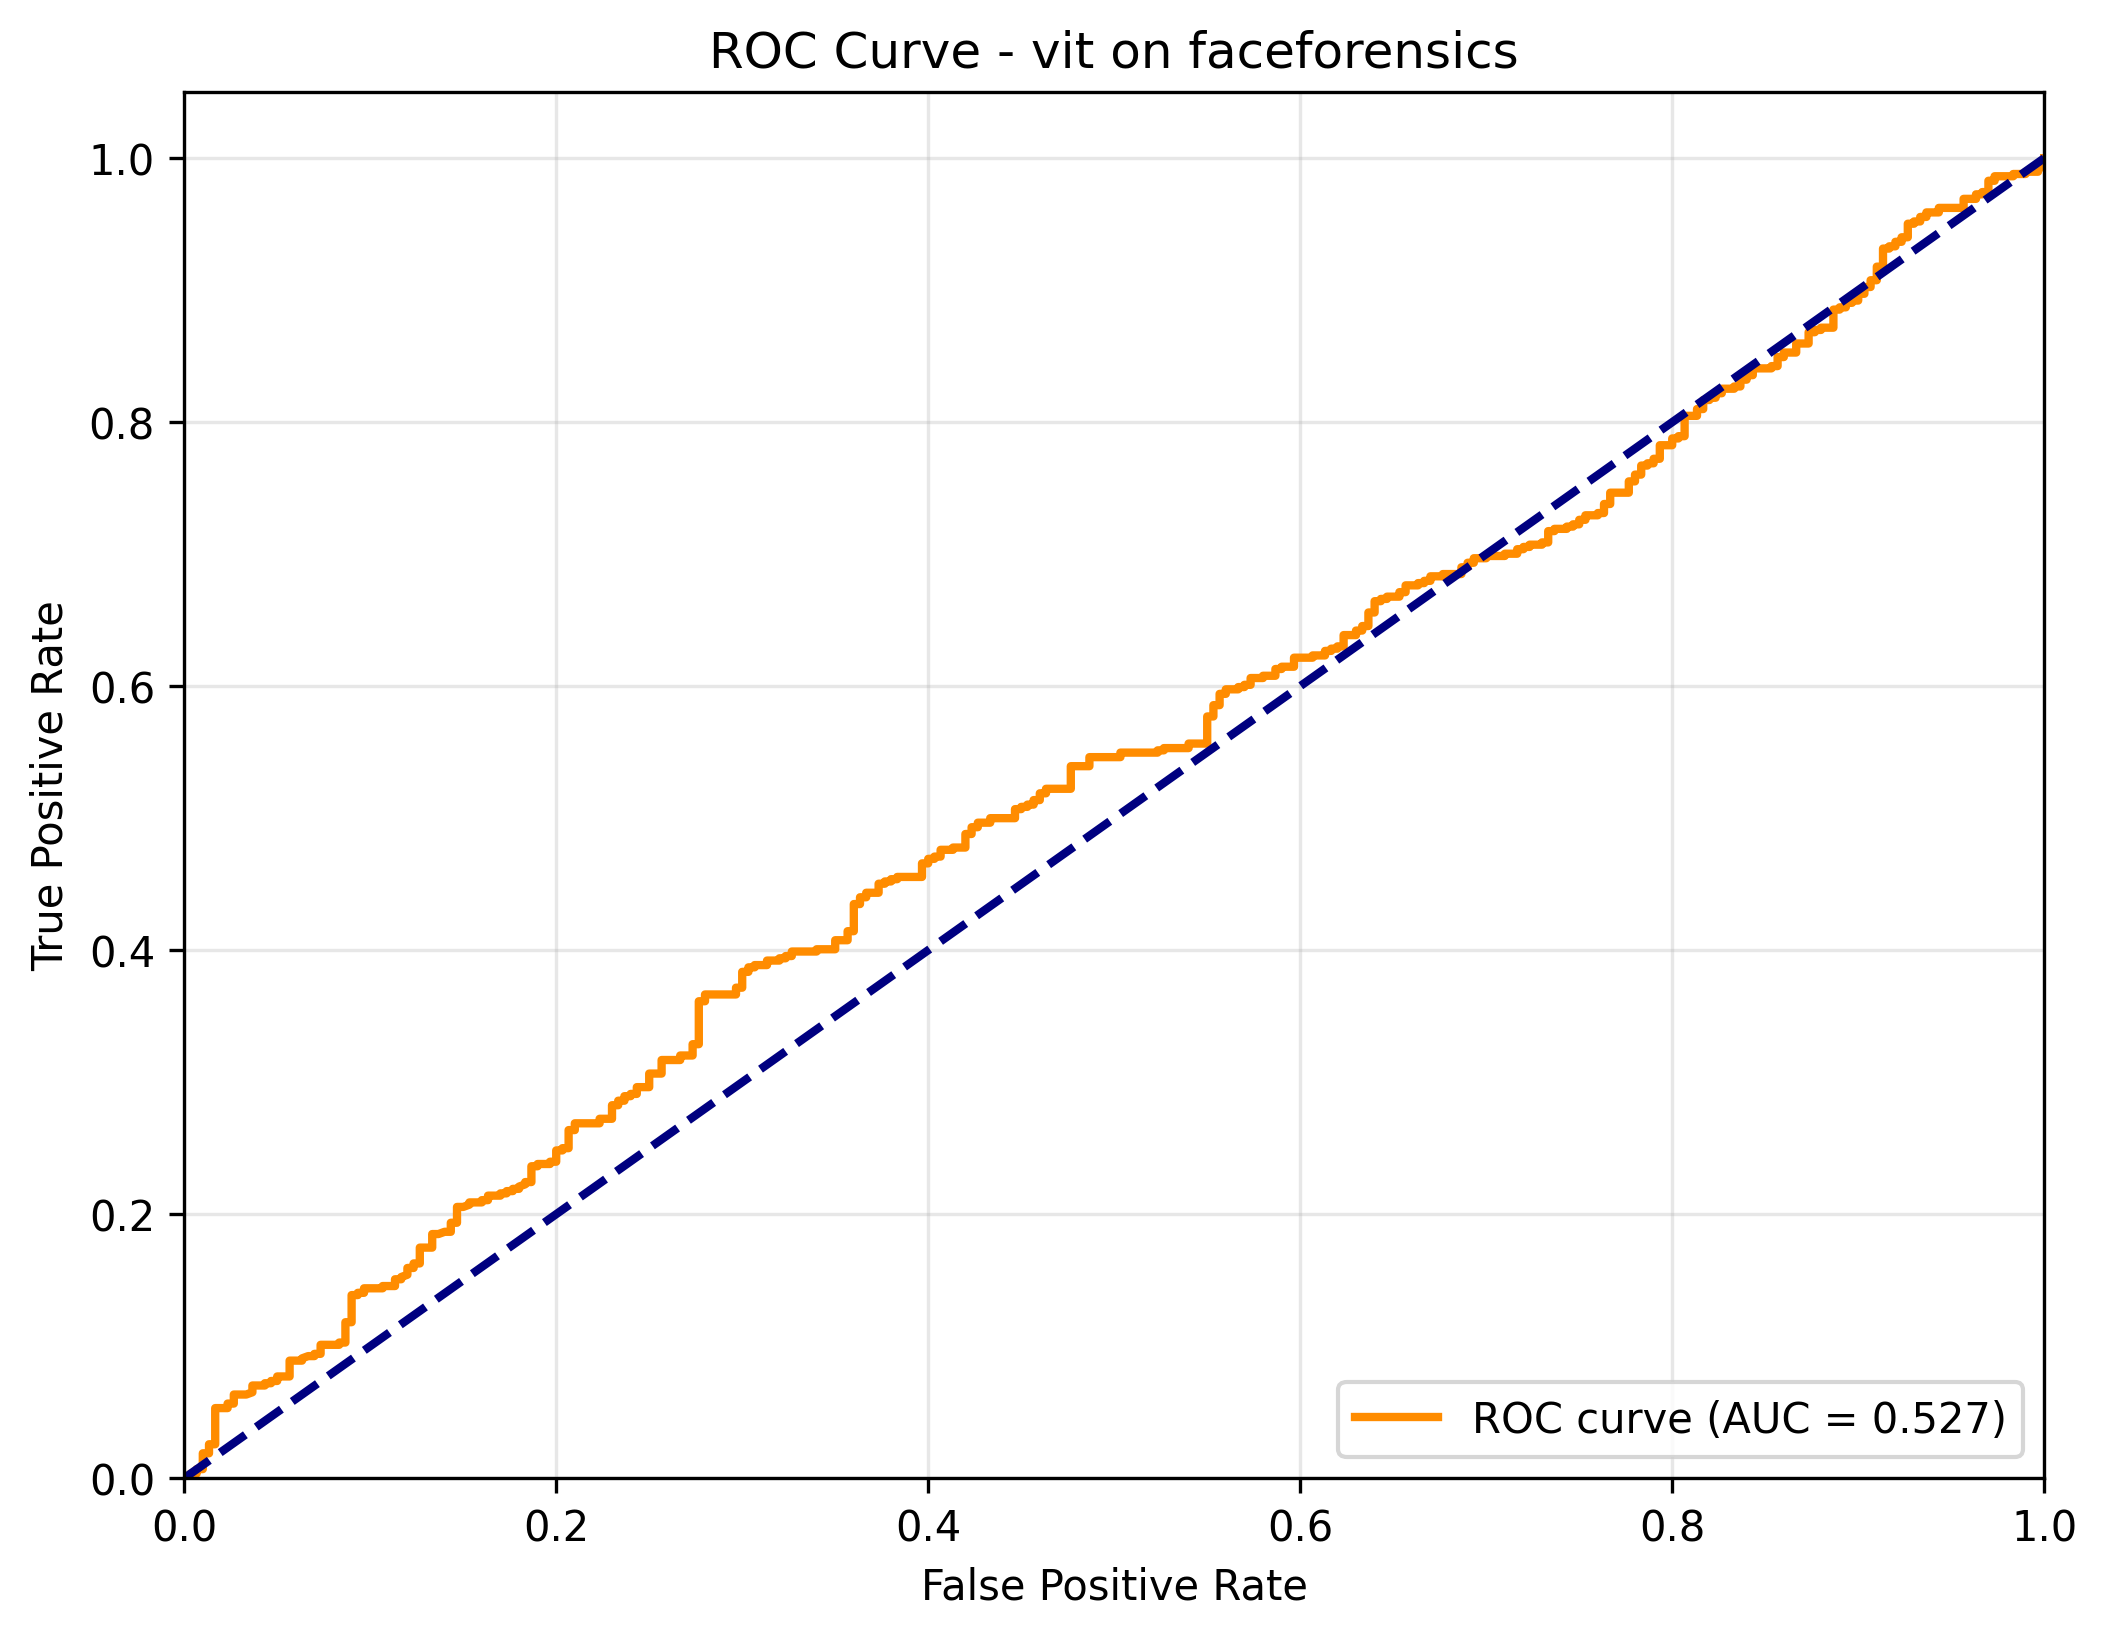
\includegraphics[width=0.20\textwidth]{figures/vit_faceforensics_roc_curve.png} \\
(c) ResNet50 & (d) Vision Transformer
\end{tabular}
\caption{ROC curves for cross-dataset evaluation (Celeb-DF trained models tested on FaceForensics++).}
\label{fig:roc_ff}
\end{figure*}

\begin{figure*}[!htbp]
\centering
\begin{tabular}{cc}
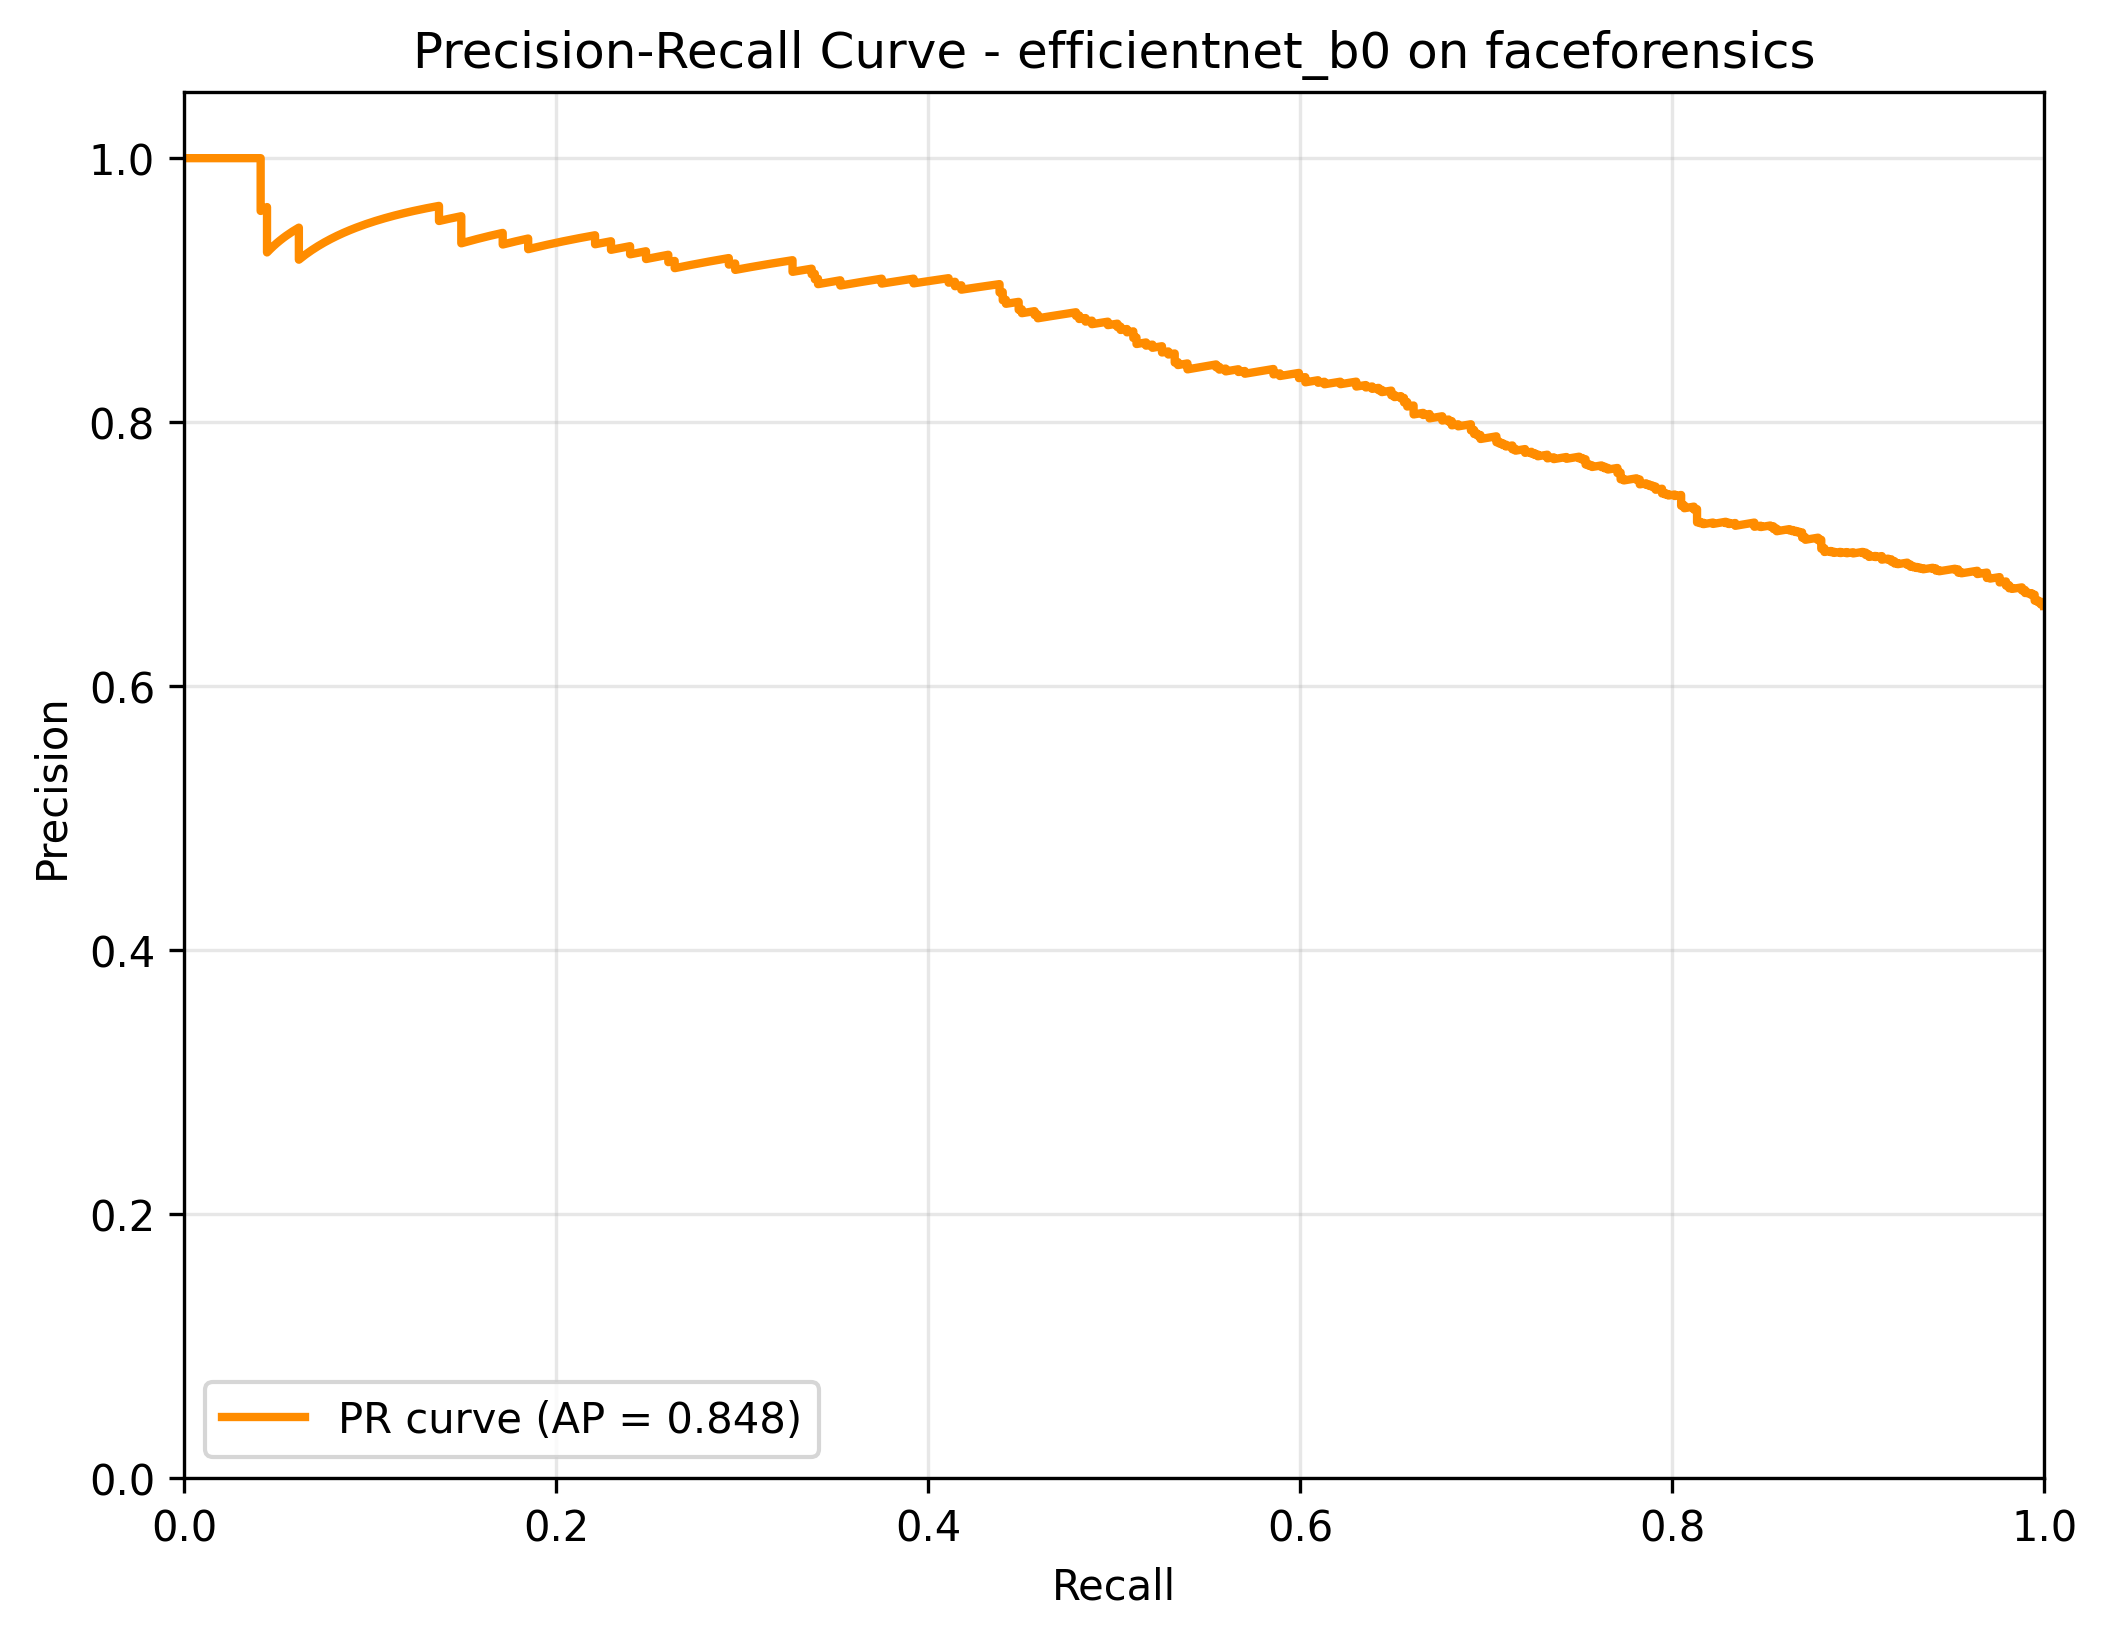
\includegraphics[width=0.20\textwidth]{figures/efficientnet_b0_faceforensics_precision_recall_curve.png} &
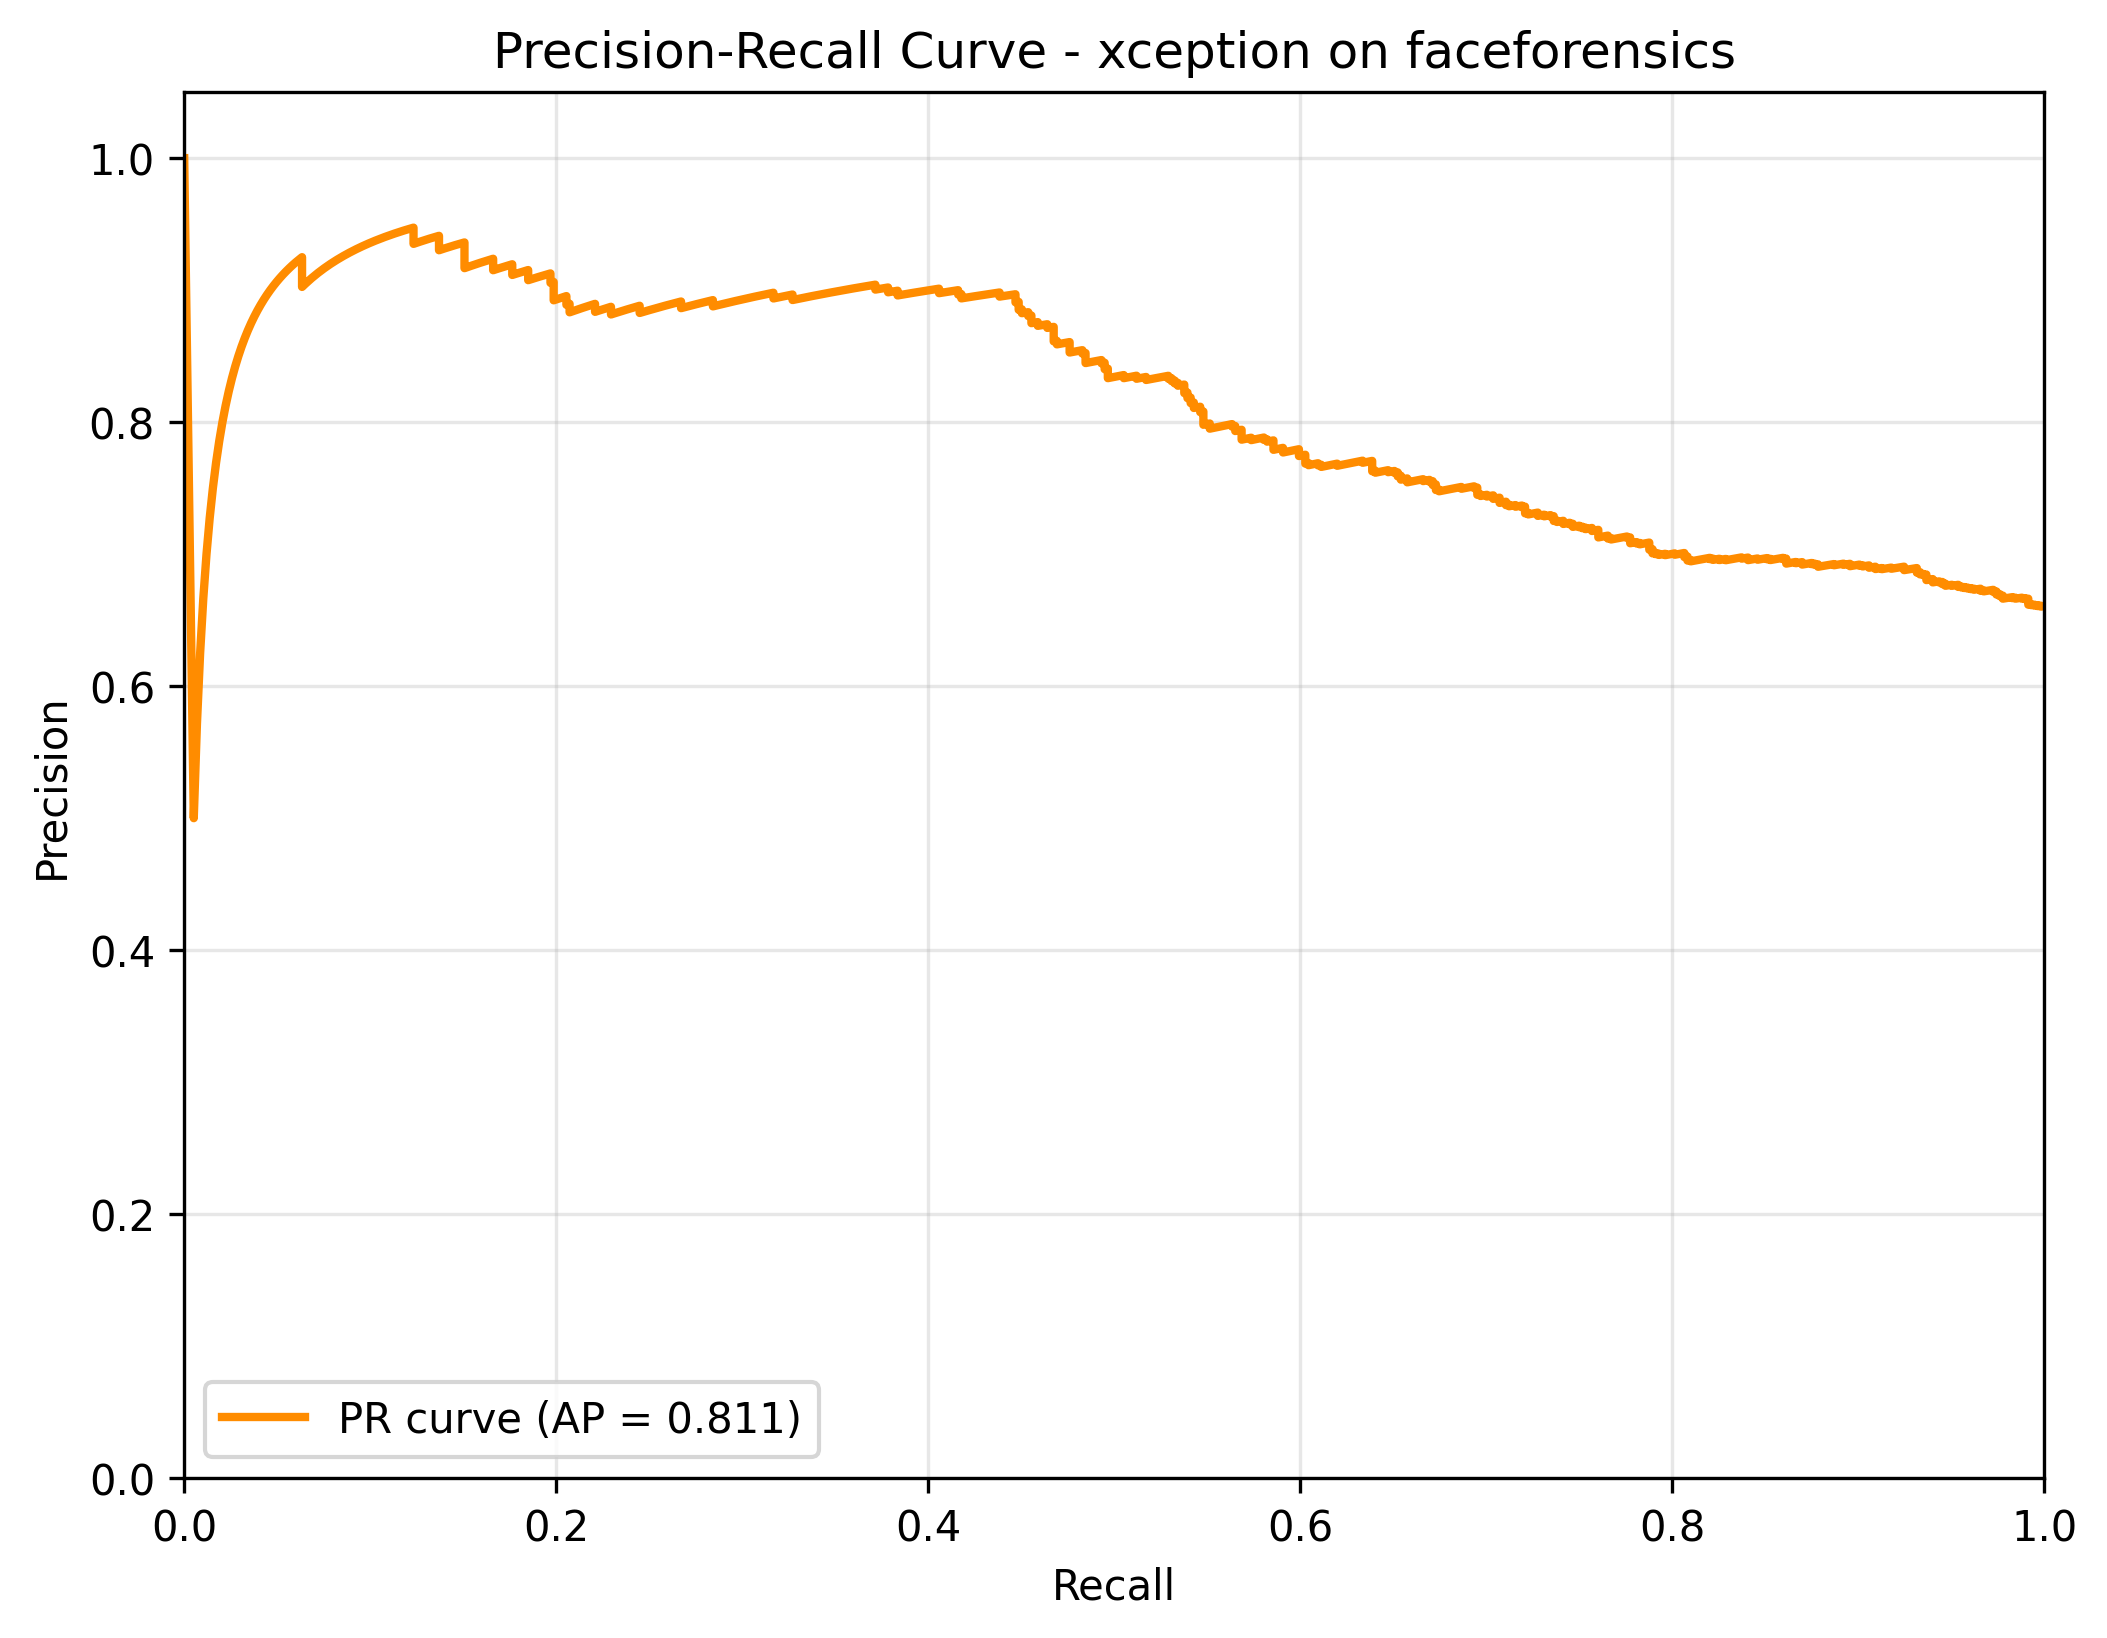
\includegraphics[width=0.20\textwidth]{figures/xception_faceforensics_precision_recall_curve.png} \\
(a) EfficientNet-B0 & (b) XceptionNet \\
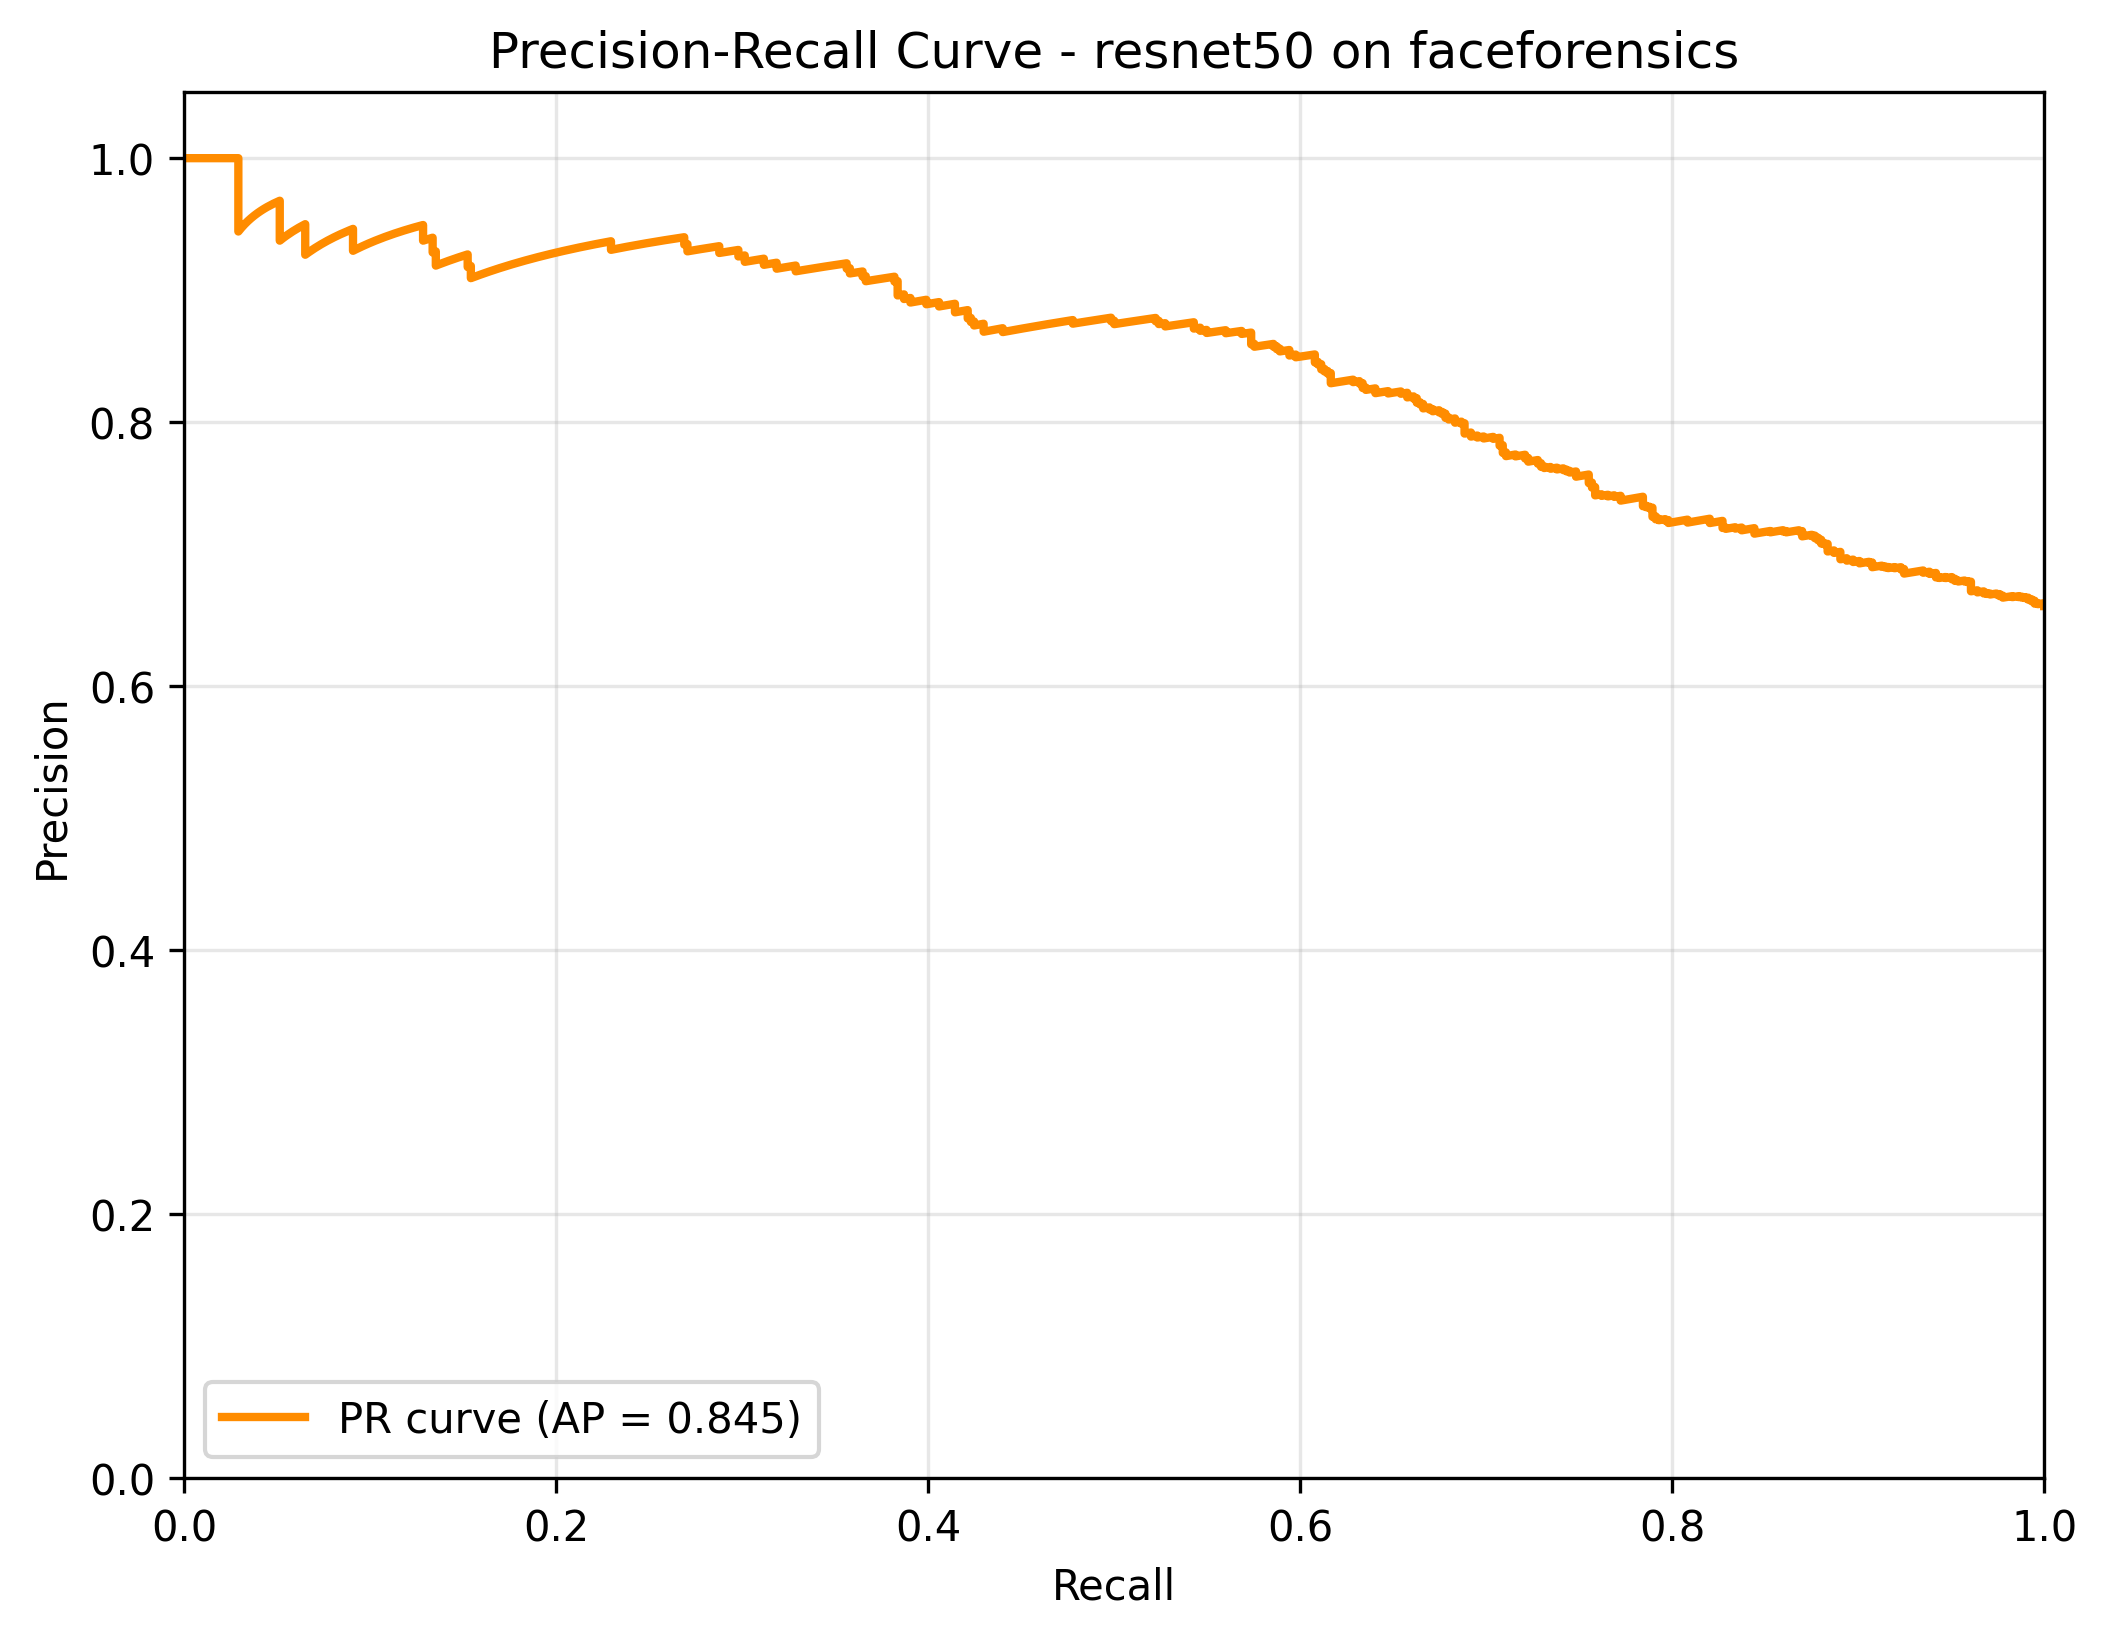
\includegraphics[width=0.20\textwidth]{figures/resnet50_faceforensics_precision_recall_curve.png} &
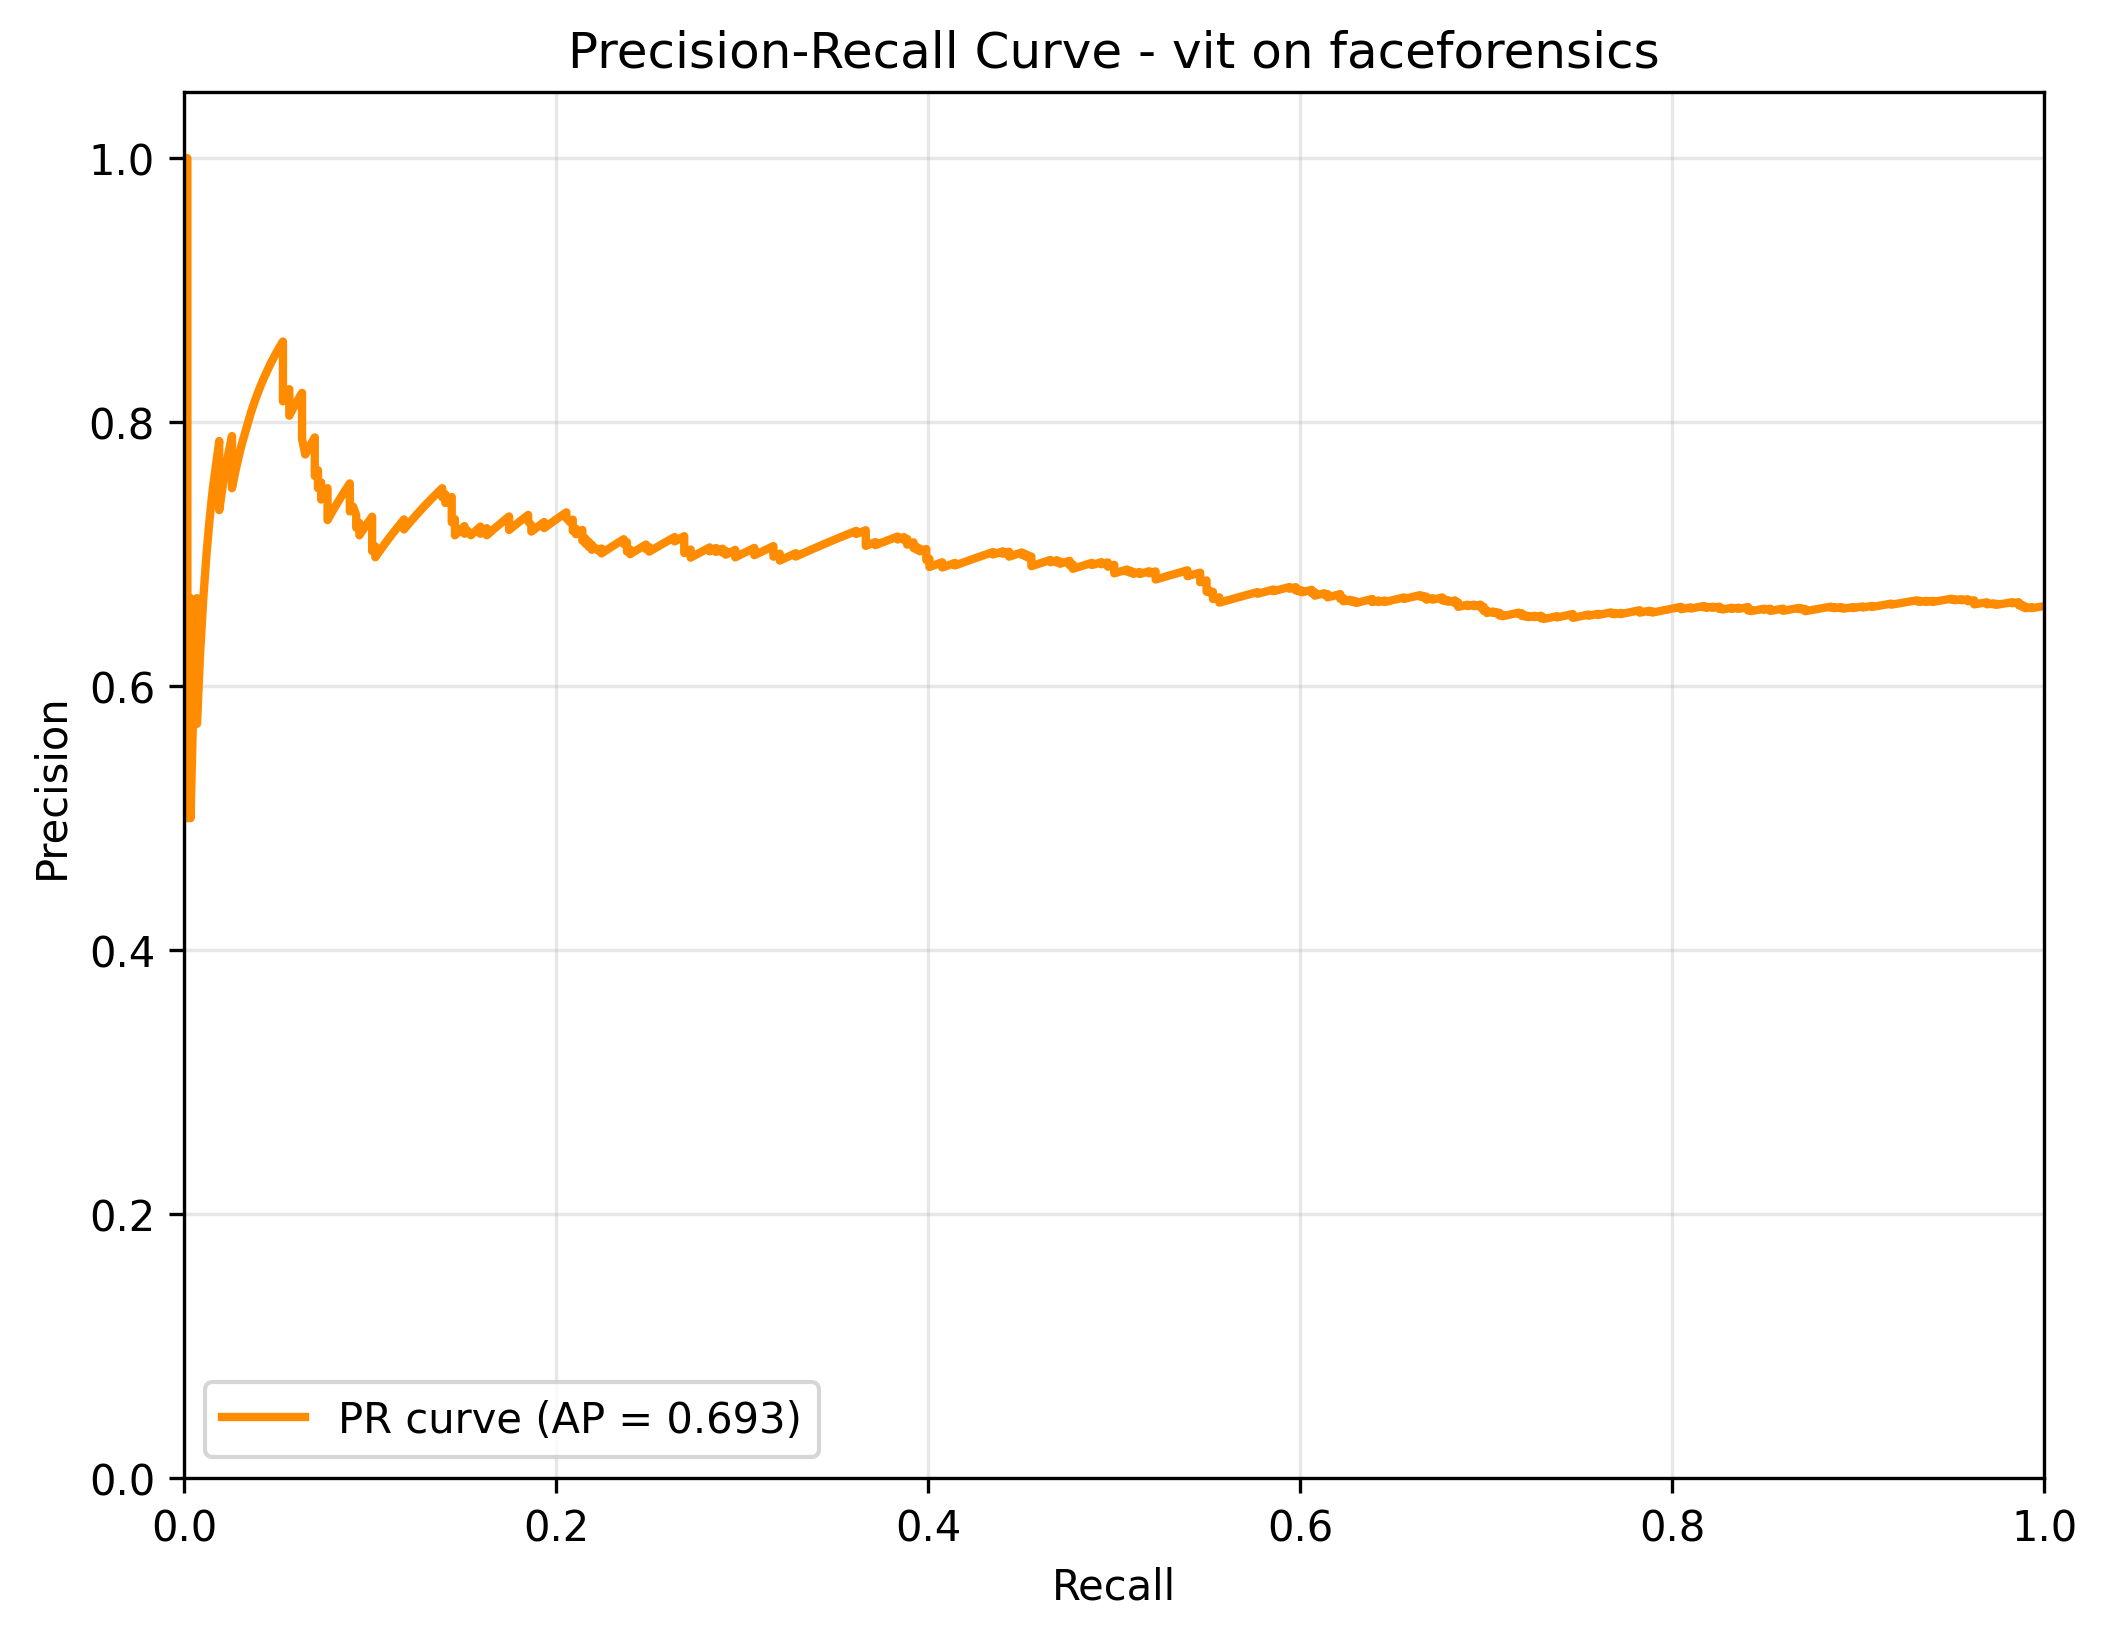
\includegraphics[width=0.20\textwidth]{figures/vit_faceforensics_precision_recall_curve.png} \\
(c) ResNet50 & (d) Vision Transformer
\end{tabular}
\caption{Precision-Recall curves for cross-dataset evaluation (Celeb-DF trained models tested on FaceForensics++).}
\label{fig:pr_ff}
\end{figure*}

When tested on FaceForensics++, the confusion matrices (Figure~\ref{fig:confusion_ff}) show a sharp increase in misclassifications. EfficientNet-B0's errors spread almost evenly across categories, dropping its accuracy to around 50\%. XceptionNet and ResNet50 follow a similar decline. The Vision Transformer's matrix, while not perfect, retains better diagonal dominance, confirming its stronger generalization. The ROC curves in Figure~\ref{fig:roc_ff} flatten noticeably, with CNN AUCs falling to 68--73\%, meaning higher true positive rates now come at the cost of many more false positives. The Precision-Recall curves in Figure~\ref{fig:pr_ff} reinforce this --- precision drops steeply as recall increases, indicating that features learned from Celeb-DF are not enough to reliably distinguish real from fake content in a different dataset.
\subsection{Model Interpretability Analysis}
\FloatBarrier

\begin{figure*}[!htbp]
\centering
\begin{tabular}{cc}
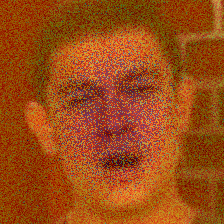
\includegraphics[width=0.12\textwidth]{figures/efficientnet_b0_gradcam_fake.png} &
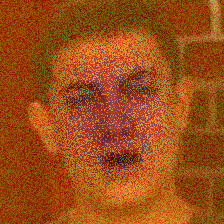
\includegraphics[width=0.12\textwidth]{figures/efficientnet_b0_gradcam_real.png} \\[-4pt]
(a) EfficientNet-B0: Fake & (b) EfficientNet-B0: Real \\[2pt]
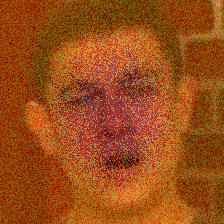
\includegraphics[width=0.12\textwidth]{figures/xception_gradcam_fake.png} &
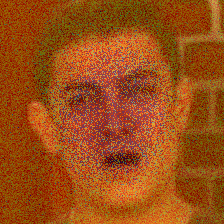
\includegraphics[width=0.12\textwidth]{figures/xception_gradcam_real.png} \\[-4pt]
(c) XceptionNet: Fake & (d) XceptionNet: Real \\[2pt]
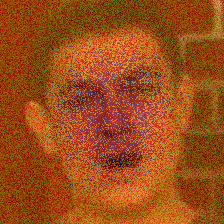
\includegraphics[width=0.12\textwidth]{figures/resnet50_gradcam_fake.png} &
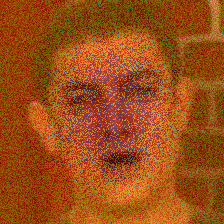
\includegraphics[width=0.12\textwidth]{figures/resnet50_gradcam_real.png} \\[-4pt]
(e) ResNet50: Fake & (f) ResNet50: Real \\[2pt]
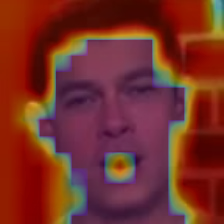
\includegraphics[width=0.12\textwidth]{figures/vit_gradcam_fake.png} &

\includegraphics[width=0.12\textwidth]{figures/vit_gradcam_real.png} \\[-4pt]
(g) Vision Transformer: Fake & (h) Vision Transformer: Real
\end{tabular}
\caption{Grad-CAM visualizations show how the model focuses its attention in all four architectures. Red regions highlight areas that are crucial for classification decisions.}
\label{fig:gradcam}
\end{figure*}

The Grad-CAM heatmaps in Figure~\ref{fig:gradcam} confirm that all four models focus on the face rather than background objects. The attention concentrates on areas like the eyes, nose, mouth, and facial contours --- common spots where manipulation artifacts appear. For fake images, the models pay more attention to facial boundaries and blending regions, while for real images the attention is more evenly spread. EfficientNet and XceptionNet show sharp, localized focus on specific features, which likely contributes to their strong in-distribution accuracy. ResNet50 and ViT have more spread-out attention patterns, covering larger facial areas. This broader view, especially in the ViT's case through its global self-attention mechanism, may explain its better generalization across different datasets.
\FloatBarrier

\subsection{Discussion}
Our experiments highlighted several key trends:

\begin{enumerate}
    \item \textbf{CNNs Dominate In-Distribution:} If the training and testing data are similar, CNNs, like EfficientNet and Xception, are the better option. They achieve nearly perfect accuracy.

    \item \textbf{The Generalization Problem:} The sharp drop in performance on FaceForensics++ shows that current models are fragile. They learn the ``fingerprint'' of a specific dataset instead of a universal definition of a deepfake.

    \item \textbf{Promise of Transformers:} Despite lower initial accuracy, the ViT's ability to withstand the significant performance drops seen in CNNs suggests that attention mechanisms capture more reliable, transferable features.

    \item \textbf{Balancing Act:} There is currently a trade-off. You can achieve high accuracy on specific data with CNNs or better stability across unknown data with ViT. Closing this gap is the next logical step.
\end{enumerate}

\textbf{ViT's Better Generalization.} Authors think this comes from basic structural differences. CNNs use local convolutional filters, which can become too specialized to features in the training data, like compression patterns or blending edges. On the other hand, ViT's self-attention mechanism looks at global relationships in the whole image. This helps it learn more abstract representations of facial inconsistencies that apply across different manipulation methods. Also, ViT's patch-based processing might be less affected by the specific spatial frequencies of individual deepfake algorithms. Instead, it captures higher-level semantic irregularities that are shared among various generation techniques.

\section{Conclusion and Future Scope}
This paper compared four deep learning architectures for deepfake detection. The results show that \textbf{CNNs like EfficientNet-B0 and XceptionNet are highly accurate on familiar data}, but their performance drops sharply when tested on unseen datasets. In contrast, the \textbf{Vision Transformer showed better resilience across datasets}, with a much smaller accuracy drop of 24.48\% compared to over 42\% for the CNNs. This suggests that the self-attention mechanism in ViTs captures more generalizable features that are not tied to a specific dataset's artifacts. Looking ahead, \textbf{ensemble methods} that combine the precision of CNNs with the robustness of ViTs could offer the best of both worlds. \textbf{Hybrid architectures} that merge convolution layers with transformer blocks are another promising direction, as they can capture both local textures and global context. Extending the analysis to \textbf{video-level detection} using temporal models like RNNs or Video Transformers, and testing against \textbf{adversarial deepfakes} designed to fool detectors, are also important next steps. Authors hope these findings contribute toward building stronger forensic tools that can keep up with the evolving landscape of synthetic media.

\section*{Acknowledgment}
The authors thank the research teams who created and maintained the Celeb-DF and FaceForensics++ datasets. These datasets have played a key role in improving deepfake detection research.

\begin{thebibliography}{00}
\bibitem{deepfake_survey} D. Güera and E. J. Delp, ``Deepfake video detection using recurrent neural networks,'' in Proc. 15th IEEE Int. Conf. Advanced Video and Signal Based Surveillance (AVSS), 2018, pp. 1--6.
\bibitem{frequency_domain} Y. Li, M. Chang, and S. Lyu, ``In ictu oculi: Exposing AI created fake videos by detecting eye blinking,'' in Proc. IEEE Int. Workshop on Information Forensics and Security (WIFS), 2018, pp. 1--7.
\bibitem{xception_deepfake} F. Chollet, ``Xception: Deep learning with depthwise separable convolutions,'' in Proc. IEEE Conf. Computer Vision and Pattern Recognition (CVPR), 2017, pp. 1251--1258.
\bibitem{efficientnet} M. Tan and Q. Le, ``EfficientNet: Rethinking model scaling for convolutional neural networks,'' in Proc. Int. Conf. Machine Learning (ICML), 2019, pp. 6105--6114.
\bibitem{resnet_deepfake} K. He, X. Zhang, S. Ren, and J. Sun, ``Deep residual learning for image recognition,'' in Proc. IEEE Conf. Computer Vision and Pattern Recognition (CVPR), 2016, pp. 770--778.
\bibitem{vit} A. Dosovitskiy et al., ``An image is worth 16x16 words: Transformers for image recognition at scale,'' in Proc. Int. Conf. Learning Representations (ICLR), 2021.
\bibitem{cross_dataset} Y. Li, X. Yang, P. Sun, H. Qi, and S. Lyu, ``Celeb-DF: A large-scale challenging dataset for deepfake forensics,'' in Proc. IEEE/CVF Conf. Computer Vision and Pattern Recognition (CVPR), 2020, pp. 3207--3216.
\bibitem{mesonet} D. Afchar, V. Nozick, J. Yamagishi, and I. Echizen, ``MesoNet: a compact facial video forgery detection network,'' in Proc. IEEE Int. Workshop on Information Forensics and Security (WIFS), 2018, pp. 1--7.
\bibitem{faceforensics} A. Rössler, D. Cozzolino, L. Verdoliva, C. Riess, J. Thies, and M. Nießner, ``FaceForensics++: Learning to detect manipulated facial images,'' in Proc. IEEE/CVF Int. Conf. Computer Vision (ICCV), 2019, pp. 1--11.
\end{thebibliography}

\end{document}
